\begin{savequote}[75mm]
Obvious is the most dangerous word in mathematics
\qauthor{--- Eric Temple Bell ---}
\end{savequote}


\chapter{Algebraic functions}
\graphicspath{{figures/Algebraic/}}
\label{chap_algebraic}

\section{Polynomial functions}
\label{sec_pol}
\subsection{Constant and linear functions}
\label{Constant_lin_fun}
Many of the functions we already encountered in the preceding chapter were either constant or linear. Here, we first of all give a more formal definition of a linear function. 

\begin{definition}[Linear function]
\label{def_lin_fun}
 A \index{function ! linear}\index{linear function} \index[aut]{lineaire functie}\index[aut]{functie ! lineair}\textbf{linear function} (\textit{lineaire functie}) is a function of the form \[ f(x) = a\,x + b,\] where $a$ and $b$ are real numbers with $a \neq 0$.  The domain of a linear function is $\mathbb{R}$.%$\left.\right]-\infty, \infty\left[\right.$.
\end{definition}


For the case $a=0$, we get $f(x) = b$, which is referred to as a \textbf{constant function} (\textit{constante functie})\index{function ! constant}\index[aut]{functie ! constant}.



Recall that to graph a function $f$, we graph the equation $y=f(x)$. Hence, the graph of a linear function is a line with slope $a$ and $y$-intercept $(0,b)$; the graph of a constant function is a horizontal line (a line with slope $a = 0$) and an $y$-intercept of $(0,b)$. For that reason, Definition~\ref{def_lin_fun} is therefore often referred to as the slope-intercept definition of a line in the plane.   In general, given two points in the plane $(x_1,y_1)$ and $(x_2,y_2)$  the equation of straight line is given by
\begin{equation}
y-y_1=\dfrac{y_2-y_1}{x_2-x_1}\left(x-x_1\right)\,,
    \label{vglrechte}
\end{equation}
where 
$$\dfrac{y_2-y_1}{x_2-x_1}$$
is the slope of the line. 


\subsection{Quadratic functions}

\begin{definition}[Quadratic function] \label{quadraticfunction} 
A \index{function ! quadratic} \index[aut]{functie ! kwadratisch} \index{quadratic function}  \textbf{quadratic function} (\textit{kwadratische functie}) is a function of the form \[ f(x) = ax^2 + bx + c,\] where $a$, $b$ and $c$ are real numbers with $a \neq 0$.  The domain of a quadratic function is $\mathbb{R}$.%$\left.\right]-\infty, \infty\left[\right.$.

\end{definition}
The most basic quadratic function is $f(x) = x^2$, which is shown in Figure~\ref{fig_algebraic_1}.  Its shape is called a \index{parabola}\index[aut]{parabool}\textbf{parabola} (\textit{parabool}). The point $(0,0)$ is called the \index{parabola ! vertex}\index[aut]{parabool ! top}\textbf{vertex} (\textit{top}) of the parabola. 

\begin{figure}[H]
	\begin{center}
			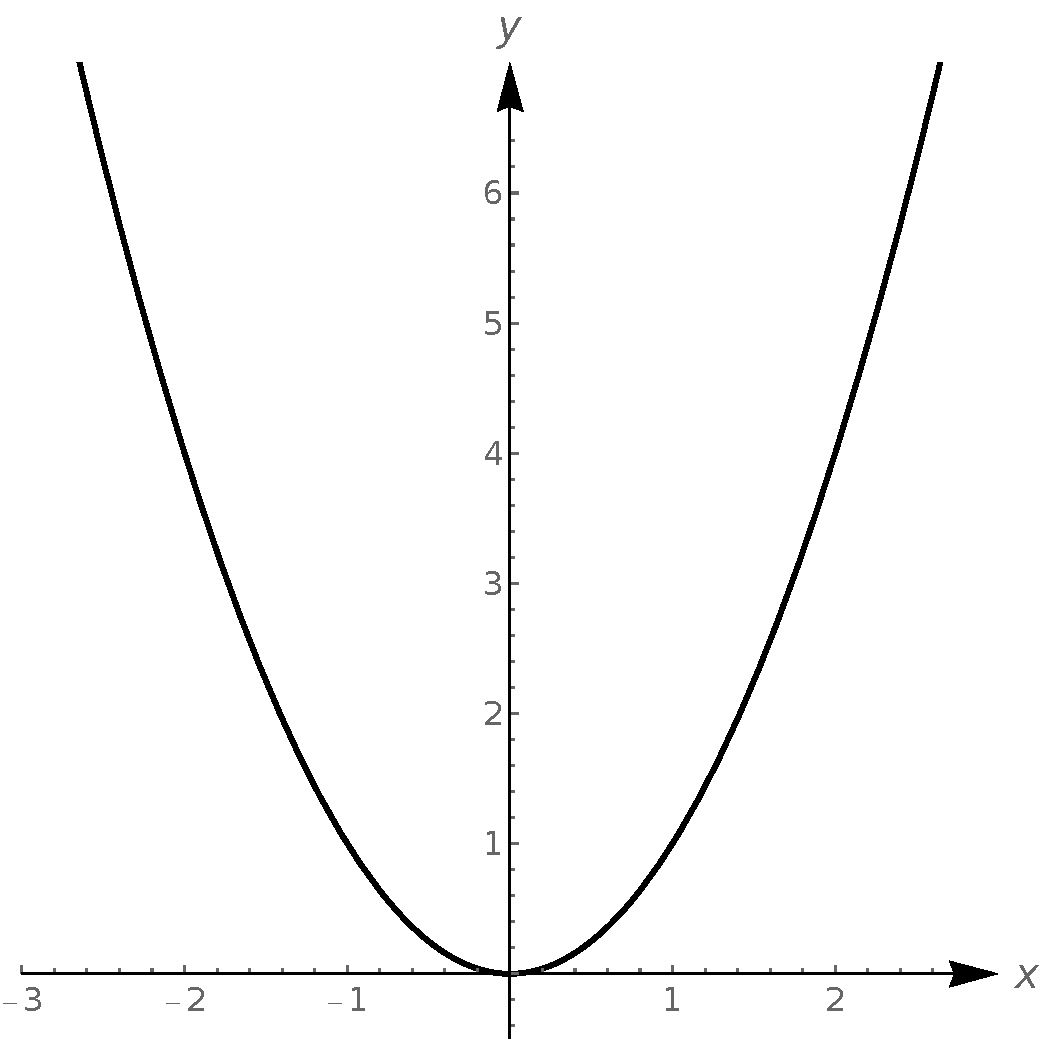
\includegraphics[width=0.3\textwidth]{fig_algebraic_1}
	\caption{The graph of $y=x^2$.}
	\label{fig_algebraic_1}
	\end{center}
\end{figure}

Definition~\ref{quadraticfunction} uses the general form of a quadratic function, though a quadratic function $f$ may as well be defined using its so-called standard form, being
$$f(x) = a(x-h)^2 + k\,,$$ 
where $a$, $h$ and $k$ are real numbers with $a\neq 0$. The vertex of the graph of $y=f(x)$ is in this notation given by $(h,k)$.  Any quadratic function can be rewritten in standard form by completing the square.

% \[ \begin{array}{rclr} 
% f(x) & = & ax^2 + bx + c & \\[10pt]
% & = & a\left(x^2 + \dfrac{b}{a} x\right) + c & \text{(Factor out coefficient of $x^2$ from $x^2$ and $x$.)} \\[15pt]
% & = &  a\left(x^2 + \dfrac{b}{a} x + \dfrac{b^{2}}{4a^2} \right)  - a \left(\dfrac{b^{2}}{4a^2}\right) + c  & \text{(Form and group the perfect square.)} \\  [15pt]
% & = & a\left(x+\dfrac{b}{2a}\right)^2 + \dfrac{4ac - b^2}{4a} & \text{(Factor and get a common denominator.)} \\ \end{array}\]



The graph of $y = a(x-h)^2 + k$ is a parabola opening upwards if $a > 0$, and opening downwards if $a < 0$. Moreover, the symmetry enjoyed by the graph of $y = x^2$ about the $y$-axis is translated to a symmetry about the vertical line $x=h=-\frac{b}{2a}$ which is the vertical line through the vertex. This line is called the \index{axis of symmetry}\index[aut]{symmetrieas}\textbf{axis of symmetry} (\textit{symmetrieas}) of the parabola. 


\ifvc
\begin{example}
Convert the function
$$f(x) = -x^2-x+6$$
 from general form to standard form.  Find the vertex, axis of symmetry and any $x$- or $y$-intercepts.  Graph the function and determine its range.

\xhrulefill{gray}{2.5pt}Solution \xhrulefill{gray}{2.5pt}

To get started, we note that the coefficient of $x^2$ is $-1$.  This means our first step is to factor out the $-1$ from both the $x^2$ and $x$ terms.  We then complete the square. \[ \begin{array}{rclr}


f(x) & = & -x^2-x+6 &  \\
	   & = & (-1)\left(x^2 + x \right) + 6 & \text{(Factor the coefficient of $x^2$ from $x^2$ and $x$.)} \\ [5pt]
		 & = & (-1)\left(x^2 + x + \dfrac{1}{4}\right) + (-1)\left(-\dfrac{1}{4}\right) + 6 & \text{(Form and group the perfect square.)}\\ [5pt]
		  & = & -\left(x +\dfrac{1}{2}\right)^2 + \dfrac{25}{4} & \\
		 \end{array} \]

From $f(x) =  -\left(x +\frac{1}{2}\right)^2 + \frac{25}{4}$, we get the vertex to be $\left(-\frac{1}{2}, \frac{25}{4}\right)$ and the axis of symmetry to be $x = -\frac{1}{2}$.  To get the $x$-intercepts, we consider $f(x) = -x^2-x+6 = 0$.  Solving, we get $x = -3$ and $x=2$ , so the $x$-intercepts are $(-3,0)$ and $(2,0)$.  Setting $x=0$, we find $f(0) = 6$, so the $y$-intercept is $(0,6)$. Plotting these points gives us the graph in Figure~\ref{fig_algebraic_2}.  We see that the range of $g$ is $\left.\right]-\infty, \frac{25}{4}\left.\right]$.

\begin{figure}[H]
	\begin{center}
			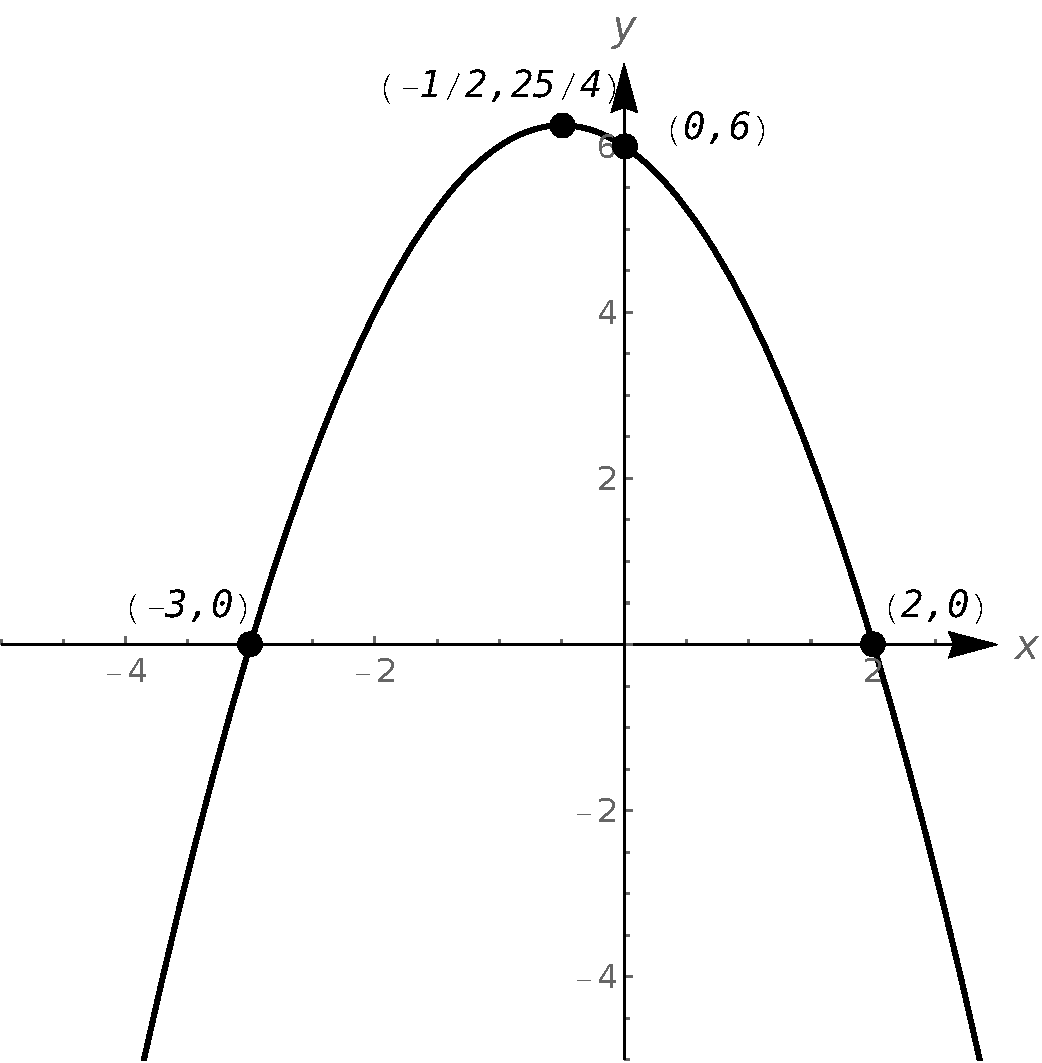
\includegraphics[width=0.3\textwidth]{fig_algebraic_2}
	\caption{The graph of $y=-x^2-x+6$.}
	\label{fig_algebraic_2}
	\end{center}
\end{figure}
\end{example}

\fi


\ifcourse
Our next example is a classic application of quadratic functions.

\begin{example}
 \label{donniealpaca} 
Donnie inherits a large parcel of land near Tielt from one of his relatives.  The time is finally right for him to pursue his dream of farming some cannabis (\textit{Cannabis sativa}).  He wishes to build a rectangular pasture, and estimates that he has enough money for 200 linear metres of fencing material.  If he makes the pasture adjacent to a stream (so no fencing is required on that side), what are the dimensions of the pasture which maximize the area?  What is the maximum area?  If an average cannabis plant needs 2.5 square metres of grazing area, how many cannabis can Donnie keep in his pasture?  It is always helpful to sketch the problem situation (Figure~\ref{fig_algebraic_3}).


\begin{figure}[H]
	\begin{center}
			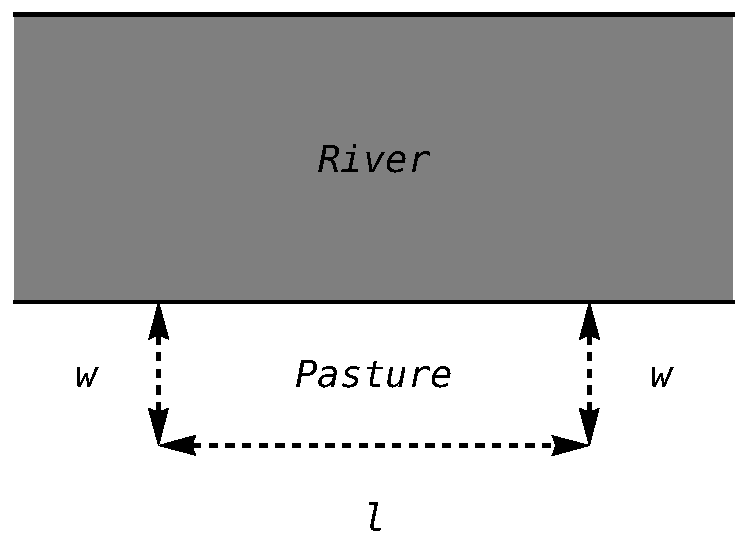
\includegraphics[width=0.3\textwidth]{fig_algebraic_3}
	\caption{Donnie's pasture.}
	\label{fig_algebraic_3}
	\end{center}
\end{figure}

\xhrulefill{gray}{2.5pt}Solution \xhrulefill{gray}{2.5pt}

We are tasked to find the dimensions of the pasture which would give a maximum area.  We let $w$ [L] denote the width of the pasture and we let $l$ [L] denote the length of the pasture.  Since the units given to us in the statement of the problem are metres, we assume $w$ and $l$ are measured in metre.  The area of the pasture, which we will call $A$, is related to $w$ and $l$ by the equation $A = wl$.  Since $w$ and $l$ are both measured in metre, $A$ [L$^2$] has units of square metre.  We are given the total amount of fencing available is $200$ metres, which means $w + l + w = 200$, or, $l+2w = 200$.  We now have two equations, 
$$
\left\{\begin{array}{rcl}
    A &=&wl\,,  \\
     l+2w&=&200\,.
\end{array}\right.
$$  In order to maximize $A$, we need to use the information given to write $A$ as a function of just one variable, either $w$ or $l$:
$$A = wl = w(200-2w) = 200w-2w^2.$$ 
We now have $A$ as a function of $w$:

$$A(w) = -2w^2+200w.$$


Before we go any further, we need to find the applied domain of $A$ so that we know what values of $w$ make sense in this problem situation. Since $w$ represents the width of the pasture, $w~>~0$.  Likewise, $l$ represents the length of the pasture, so $l = 200-2w~>~0$.  Solving this latter inequality, we find $w < 100$.  Hence, the function we wish to maximize is $A(w) = -2w^2 + 200w$ for $0~<~w~<~100$.  Since $A$ is a quadratic function of $w$, we know that the graph of $y = A(w)$ is a parabola.  Since the coefficient of $w^2$ is $-2$, we know that this parabola opens downwards.  This means that there is a maximum value to be found, and we know it occurs at the vertex.  Using the vertex formula, we find 
$$
\left\{\begin{array}{rcl}
    w &=& -\dfrac{200}{2(-2)} = 50\,,  \\[0.2cm]
     A(50)& =& -2(50)^2 + 200(50) = 5000\,.
\end{array}\right.
$$ 
  Since $w=50$ lies in the applied domain, $0~<~w~<~100$, we have that the area of the pasture is maximized when the width is $50$ metres.  To find the length, we use $l = 200-2w$ and find $l = 200-2(50) = 100$, so the length of the pasture is $100$ metres.  The maximum area is $A(50) = 5000$, or $5000$ m$^2$.  If an average cannabis plant requires 2.5 square metres of pasture, Donnie can raise $\frac{5000}{2.5} = 2000$ such plants. 

\end{example}
\fi

In practice, quadratic functions often pop up in inequalities, which we can solve graphically.


\ifvc
\begin{example}
 Solve the following inequalities graphically.

\begin{multicols}{2}
\begin{enumerate}

\item  $2x^2 \leq 3-x$

\item  $x^2 - 2x > 1$

\end{enumerate}
\end{multicols}
\xhrulefill{gray}{2.5pt}Solution \xhrulefill{gray}{2.5pt}

 
\begin{enumerate}

\item  To solve the inequality graphically, we let $g(x) = 2x^2$ and $h(x)=3-x$.  We are looking for the $x$-values where the graph of $g$ is below that of $h$ (the solution to $g(x) < h(x)$) as well as the points of intersection (the solutions to $g(x)=h(x)$). The latter can be found easily by solving the system
$$
\left\{\begin{array}{rcl}
y & = & 2x^2\\[.1cm]
y & = & 3-x\,,
\end{array}\right.
$$
which yields $(-3/2, 9/2)$ and $(1,2)$. The graphs of $g$ and $h$ and the resulting solution interval, $\left[-3/2,1\right]$ , are given in Figure~\ref{fig_algebraic_4}. 
\begin{figure}[H]
    \begin{center}
			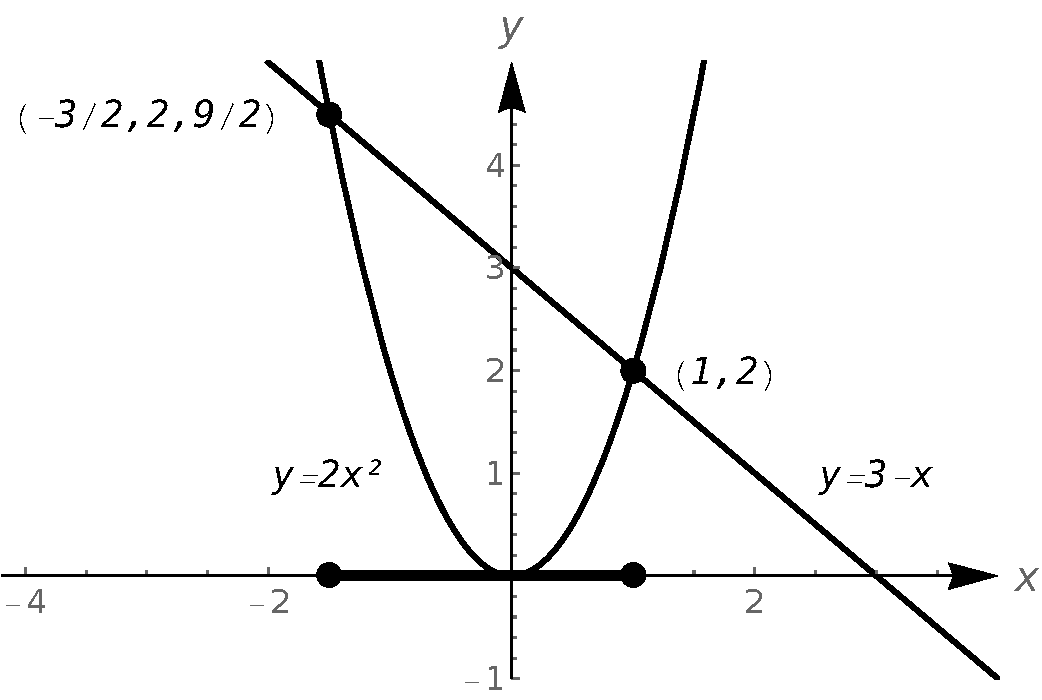
\includegraphics[width=0.4\textwidth]{fig_algebraic_4}
	\caption{Graphs of $g(x) = 2x^2$ and $h(x)=3-x$ and solution interval of $2x^2 \leq 3-x$.}
	\label{fig_algebraic_4}
	\end{center}
\end{figure}

	
\item  To check the inequality $x^2 - 2x > 1$ graphically, we set $g(x) = x^2-2x$ and $h(x)=1$.  We are looking for the $x$ values where the graph of $g$ is above the graph of $h$. The points of intersection can be found by solving the system
$$
\left\{
\begin{array}{rcl}
y & = & x^2-2x\\[.1cm]
y & = & 1\,,
\end{array}\right.
$$
which yields $(1-\sqrt{2}, 1)$ and $(1+\sqrt{2},1)$.  The graphs of $g$ and $h$ and the resulting solution interval, $\left.\right]-\infty,1-\sqrt{2}\left[\right. \cup \left.\right]1+\sqrt{2},+\infty\left[\right.$, are given in Figure~\ref{fig_algebraic_5}.

\begin{figure}[H]
    \begin{center}
			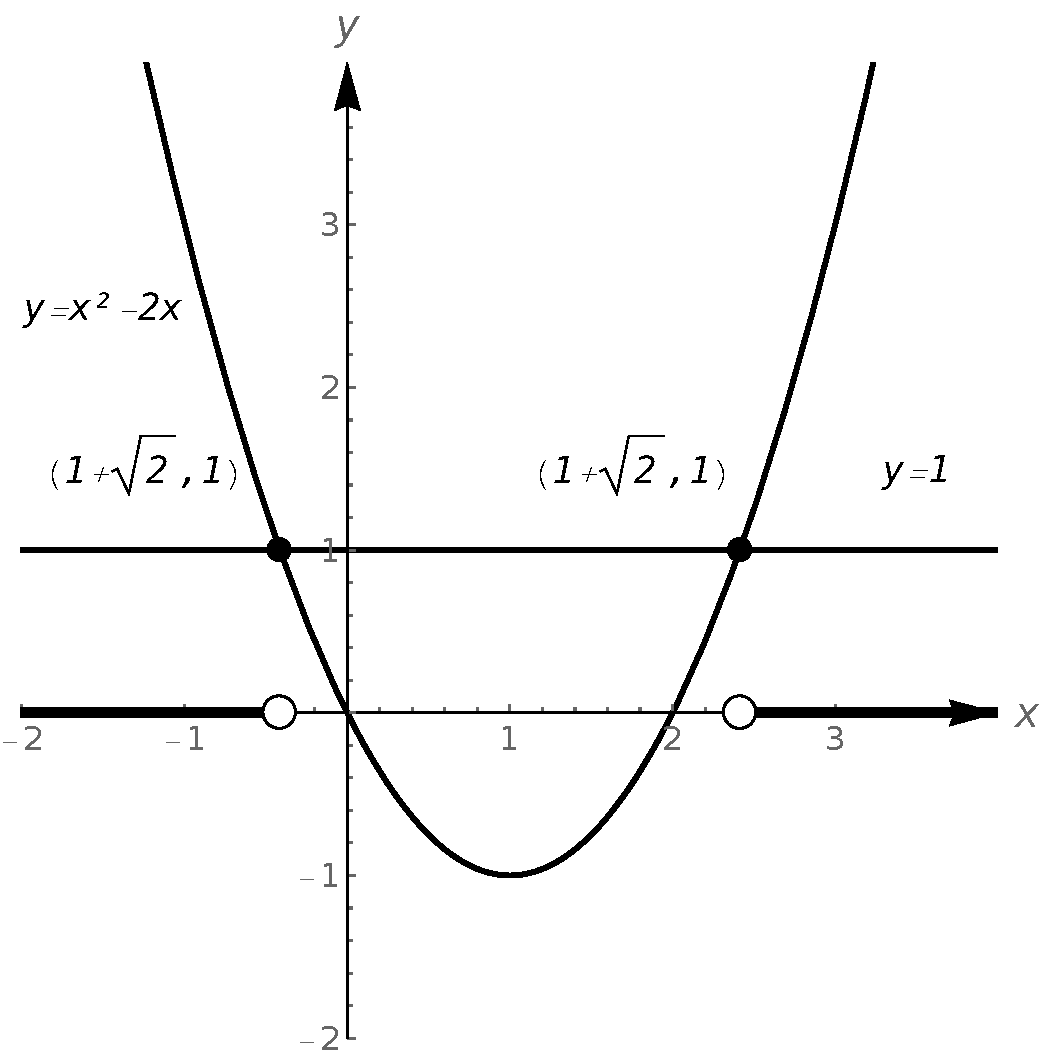
\includegraphics[width=0.3\textwidth]{fig_algebraic_5}
	\caption{Graphs of $g(x) = x^2-2x$ and $h(x)=1$ and solution interval of $x^2 - 2x > 1$.}
	\label{fig_algebraic_5}
	\end{center}
\end{figure}


	
\end{enumerate}	
	
\end{example}
\fi

\ifcourse
One of the classic applications of inequalities is the notion of \textbf{tolerances}.  Recall that for real numbers $x$ and $c$, the quantity $|x-c|$ may be interpreted as the distance from $x$ to $c$.  Solving inequalities of the form $|x-c| \leq d$ for $d \geq 0$ can then be interpreted as finding all numbers $x$ which lie within $d$ units of $c$.  We can think of the number $d$ as a tolerance and our solutions $x$ as being within an accepted tolerance of $c$.  We use this principle in the next example.

\begin{example} 
The area $A$ ([L$^2$]) of a square piece of particle board which measures $x$ [L] centimetres on each side is $A(x) = x^2$.  Suppose a manufacturer needs to produce a $24$ centimetre by $24$ centimetre square piece of particle board as part of a home office desk kit. How close does the side of the piece of particle board need to be cut to $24$ centimetres to guarantee that the area of the piece is within a tolerance of $0.25$ square centimetres of the target area of $576$ square centimetres?  

\xhrulefill{gray}{2.5pt}Solution \xhrulefill{gray}{2.5pt}

 Mathematically, we express the desire for the area $A(x)$ to be within $0.25$ square centimetres of $576$ as $|A - 576| \leq 0.25$.  Since $A(x) = x^2$, we get $|x^2 - 576| \leq 0.25$, which is equivalent to $-0.25 \leq x^2 - 576 \leq 0.25$.  Recalling the increasing property of the square root; that is  if $0 \leq a \leq b$, then $\sqrt{a} \leq \sqrt{b}$, we proceed

\[ \begin{array}{rrclr}

&-0.25  \leq & x^2 - 576 & \leq 0.25 & \\
\Leftrightarrow&575.75 \leq & x^2 & \leq 576.25 & \quad\text{(Add $576$ across the inequalities.)} \\
\Leftrightarrow&\sqrt{575.75} \leq & \sqrt{x^2} & \leq \sqrt{576.25} & \quad\text{(Take square roots.)} \\
\Leftrightarrow&\sqrt{575.75} \leq & |x| & \leq \sqrt{576.25} & \quad\text{($\sqrt{x^2} = |x|$)} \\ \end{array} \]



Consequently, we find the solution to $\sqrt{575.75} \leq |x|$ to be $\big]-\infty, -\sqrt{575.75} \, \big] \cup \big[\sqrt{575.75}, +\infty \big[$ and the solution to $|x| \leq \sqrt{576.25}$ to be  $\big[-\sqrt{576.25}, \sqrt{576.25} \, \big]$. To solve $\sqrt{575.75} \leq  |x|  \leq \sqrt{576.25}$, we intersect these two sets to get $\big[-\sqrt{576.25}, -\sqrt{575.75}\big] \cup \big[\sqrt{575.75},\sqrt{576.25}\big]$.  Since $x$ represents a length, we discard the negative answers and get $\big[\sqrt{575.75},\sqrt{576.25}\big]$.  This means that the side of the piece of particle board must be cut between $\sqrt{575.75} \approx 23.995$ and $\sqrt{576.25} \approx 24.005$ centimetres, a tolerance of (approximately) $0.005$ centimetres of the target length of $24$ centimetres. 

\end{example}


Our last example in the section demonstrates how inequalities can be used to describe regions in the plane.

\begin{example}  
Sketch the following relations. 

\begin{multicols}{2}
\begin{enumerate}

\item $R = \{ (x,y) : y > |x| \}$

\item $S = \{ (x,y) :  y \leq 2-x^2 \}$


\end{enumerate}
\end{multicols}

\xhrulefill{gray}{2.5pt}Solution \xhrulefill{gray}{2.5pt}

\begin{enumerate}

\item  The relation $R$ consists of all points $(x,y)$ whose $y$-coordinate is greater than $|x|$.  If we graph $y=|x|$, then we want all of the points in the plane above the points on the graph.  Dotting the graph of $y=|x|$ to indicate that the points on the graph itself are not in the relation, we get the shaded region in Figure~\ref{fig_algebraic_6a}.


\item  For a point to be in $S$, its $y$-coordinate must be less than or equal to the $y$-coordinate on the parabola $y=2-x^2$.  This is the set of all points below or on the parabola $y=2-x^2$ (Figure~\ref{fig_algebraic_6b}).


\end{enumerate}

\begin{figure}[H]
\centering
%\raisebox{0.5cm}{
\centerline{
\subfigure[\label{fig_algebraic_6a}]{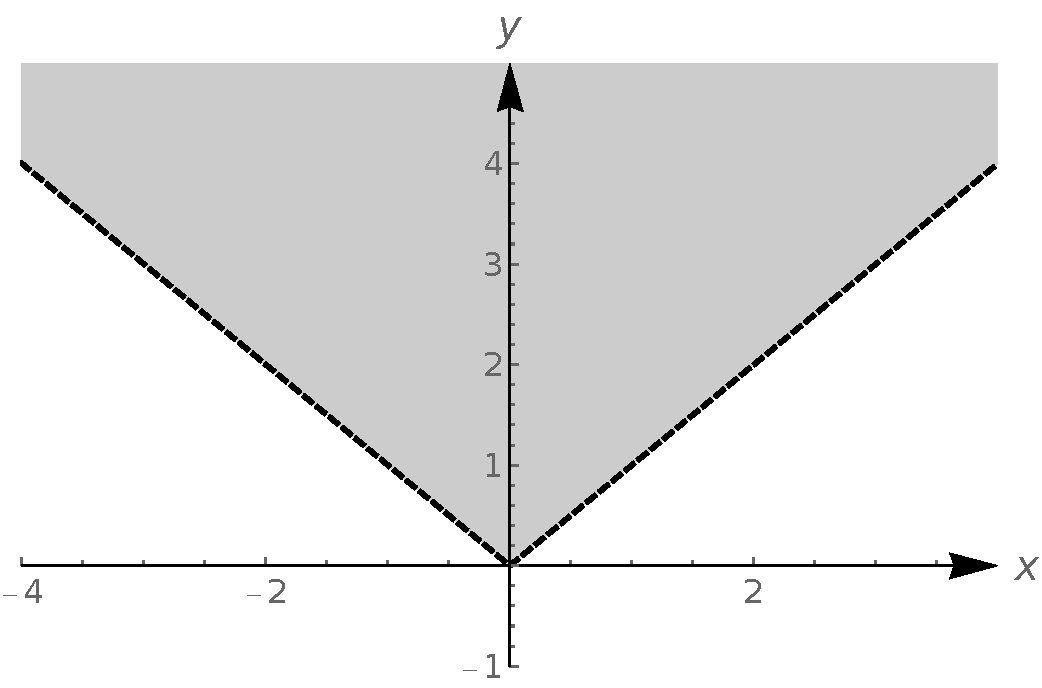
\includegraphics[width=0.4\textwidth]{fig_algebraic_6a}}
\hspace{0.1cm}
\subfigure[ \label{fig_algebraic_6b}]{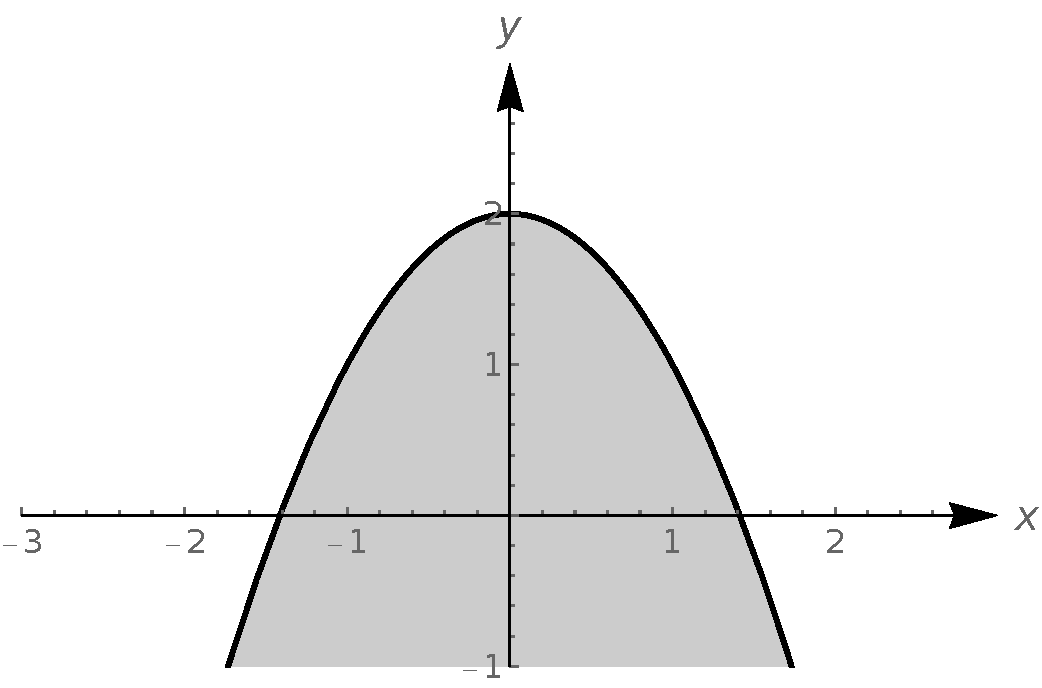
\includegraphics[width=0.4\textwidth]{fig_algebraic_6b}}
}
\caption{Graph of the relation $R$ (a) and $S$ (b). }
\end{figure}

\end{example}
\fi


Many quadratic equations $ax^2 + bx + c = 0$ cannot be solved by factoring them. This is generally true when the roots are not rational numbers. An other method of solving quadratic equations involves the use of the quadratic formula: 
\begin{equation}
 x = \dfrac{-b \pm \sqrt{b^2-4ac}}{2a}\,,
 \label{quadraticf}
\end{equation}
 where $a \neq 0$.
In relation to quadratic equations, complex numbers come in when the value under the radical portion of the quadratic formula is negative. When this occurs, the equation has no roots in $\mathbb{R}$. The roots belong to $\mathbb{C}$, will be called \textbf{complex roots} (\textit{complexe wortels}) (or imaginary roots), and are expressible as  $a\pm bi$. When using the quadratic formula to solve a quadratic equation with real coefficients, there are three possibilities depending on the discriminant $D=b^2-4ac$:
\begin{enumerate}
\item Two different real roots if $D>0$.
\item One real root if $D=0$.
\item Two complex roots, complex conjugates, if $D<0$.
\end{enumerate}


\begin{example}
Solve the following quadratic equations.
\begin{multicols}{2}
\begin{enumerate}
\item $x^2+2x+2=0$
\item $x^2-4x+13=0$
\end{enumerate}
\end{multicols}


\xhrulefill{gray}{2.5pt}Solution \xhrulefill{gray}{2.5pt}


\begin{enumerate}
	\item Substituting in Equation~\eqref{quadraticf}, we get
	\[ x = \dfrac{-b \pm \sqrt{b^2-4ac}}{2a} =  \dfrac{-2 \pm \sqrt{-4}}{2}.   \]
	Since the discriminant $D=b^2-4ac$ is negative, this equation has no solution in $\mathbb{R}$.	But if you were to express the solution using imaginary numbers, the solutions would be 
	\[x = \dfrac{-2 \pm 2i}{2} = -1 \pm i.\]
	
	\item Notice that after substitution in Equation~\eqref{quadraticf}, we are left with a negative value under the square root radical.
	\[x = \dfrac{4 \pm \sqrt{-36}}{2}  \]
	There are two complex roots
	\[x = \dfrac{4 \pm 6i}{2} = 2 \pm 3i.\]
\end{enumerate}


\end{example}


\subsection{General polynomial functions}
\subsubsection{Definition}

Three of the families of functions studied thus far -- constant, linear and  quadratic -- belong to a much larger group of functions called polynomials.  We begin our formal study of general polynomials with a definition and some examples.
%
%\pagebreak
\begin{definition}[Polynomial function] \label{polynomialfunction} 
A \index{function ! polynomial}\index{polynomial function}\index[aut]{functie ! veelterm}\index[aut]{veeltermfunctie}\textbf{polynomial function} (\textit{veeltermfunctie}) is a function of the form \[ f(x) = a_{n} x^{n} + a_{n-1} x^{n-1} + \cdots + a_{2} x^{2} + a_{1} x + a_{0},\] where $a_{0}$, $a_{1}$, \ldots, $a_{n}$ are real numbers, $a_{n} \neq 0$ and $n \in \mathbb{N}$.  The domain of a polynomial function is $\mathbb{R}$.%$\left.\right]-\infty, \infty\left[\right.$.

\end{definition}



Given $f(x) = a_{n} x^{n} + a_{n-1} x^{n-1} + \cdots + a_{2} x^{2} + a_{1} x + a_{0}$ with $a_{n} \neq 0$, we say 

\begin{itemize}

\item  The natural number $n$ is called the \index{polynomial function ! degree}\index[aut]{veeltermfunctie ! graad}\textbf{degree} (\textit{graad}) of the polynomial $f$.

\item  $a_{n} x^{n}$ is called the \index{polynomial function ! leading term}\textbf{leading term} (\textit{hoogstegraadsterm}) of the polynomial $f$.

\item  The real number $a_{n}$ is called the \index{polynomial function ! leading coefficient}\textbf{leading coefficient} of the polynomial $f$.

\item  The real number $a_{0}$ is called the \index{polynomial function ! constant term} \index[aut]{veeltermfunctie ! constante term} \textbf{constant term} (\textit{constante term}) of the polynomial $f$.

\end{itemize}

Moreover, if $f(x) = a_0$, and $a_0 \neq 0$, we say $f$ has degree $0$, while if $f(x) = 0$, we say $f$ has no degree.

\ifvc
Our next example shows how polynomials of higher degree arise naturally in even the most basic geometric applications.

\begin{example}  
 A box with no top is to be fashioned from a $10$ centimetres by $12$ centimetres piece of cardboard by cutting out congruent squares from each corner of the cardboard and then folding the resulting tabs (Figure~\ref{fig_algebraic_7}).  Let $x$ denote the length of the side of the square which is removed from each corner.  Find the volume $V$ of the box as a function of $x$.  Include an appropriate applied domain.
 
 \begin{figure}[H]
\centering
%\raisebox{0.5cm}{
\centerline{
\subfigure[\label{fig_algebraic_7a}]{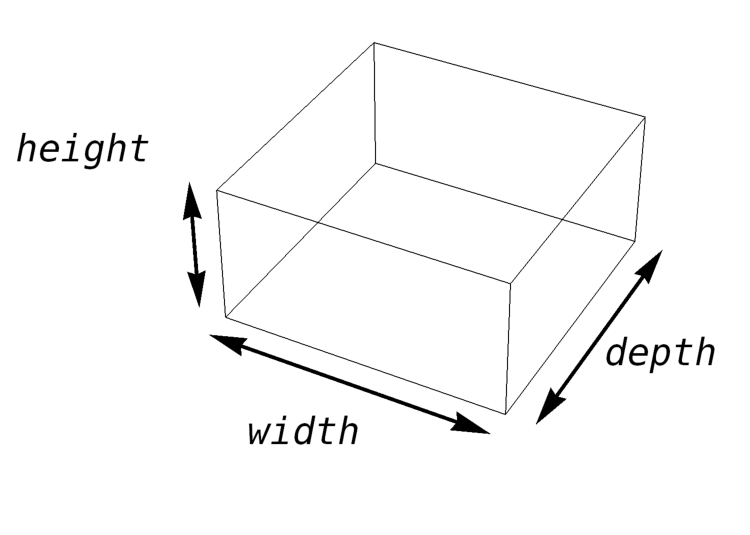
\includegraphics[width=0.4\textwidth]{fig_algebraic_7a}}
\hspace{0.5cm}
\subfigure[ \label{fig_algebraic_7b}]{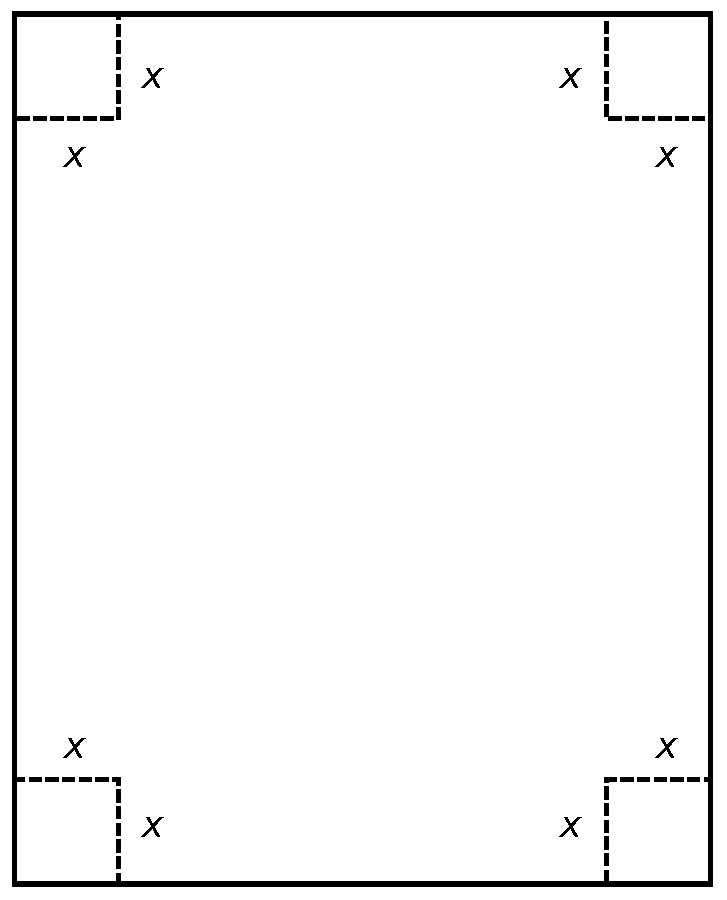
\includegraphics[width=0.2\textwidth]{fig_algebraic_7b}}
}
\caption{Constructing a box with no top. }
\label{fig_algebraic_7}
\end{figure}


\xhrulefill{gray}{2.5pt}Solution \xhrulefill{gray}{2.5pt}

We know that $\mbox{Volume} = \mbox{width} \times \mbox{height} \times \mbox{depth}$.  The key is to find each of these quantities in terms of $x$.  From the figure, we see that the height of the box is $x$ itself.  The cardboard piece is initially $10$ centimetres wide.  Removing squares with a side length of $x$ centimetres from each corner leaves $10-2x$ centimetres for the width.  As for the depth, the cardboard is initially $12$ centimetres long, so after cutting out $x$ centimetres from each side, we would have $12-2x$ centimetres remaining.   As a function of $x$, the volume is \[V(x) = x(10-2x)(12-2x) = 4x^3-44x^2+120x.\] To find a suitable applied domain, we note that to make a box at all we need $x > 0$.  Also the shorter of the two dimensions of the cardboard is $10$ centimetres, and since we are removing $2x$ centimetres from this dimension, we also require $10 - 2x > 0$ or $x < 5$.  Hence, our applied domain is $0 < x < 5$.

\end{example} 
\fi

\ifcourse In Part~\ref{deel2}, we will introduce the tools that are needed to graph polynomial functions and understand their behaviour. Anyhow, we will often have to determine the zeros of a polynomial equation. For that reason, we recall the most important facts about the factorization of polynomials. 
\fi

\subsubsection{Factorization of polynomials}
Suppose we wish to find the zeros of $f(x) = x^3 + 4x^2-5x-14$.  Setting $f(x)=0$ results in the polynomial equation $x^3 + 4x^2-5x-14=0$.    It is easy to see that $f(2) = 0$, but possible other zeros seem less obvious. Now, if $x=2$ is a zero, there should be a factor of $(x-2)$ lurking around in the factorization of $f(x)$.  In other words, we should expect that $x^3 + 4x^2-5x-14=(x-2) \, q(x)$, where $q(x)$ is some second degree polynomial. We can find this polynomial through \textbf{polynomial division} (\textit{Euclidische deling}). Dividing $x^3 + 4x^2-5x-14$ by $x-2$ gives

\setlength\arraycolsep{0.1pt}
\setlength\extrarowheight{2pt}


\[ \begin{array}{rccccccccl}

&x^3&+&4x^2&-&5x&-&14\, \,&\vline&\, \,x-2\\
\cline{9-10}-&\left(x^3\right.&-&\left.2x^2\right)&&&&&\vline&\, \,x^2+6x+7\\
\cline{1-8}&&&6x^2&-&5x&&&\vline&\\
&&-&\left(6x^2\right.&-&\left.12x\right)&&&\vline&\\
\cline{1-8}&&&&&7x&-&14&\vline&\\
&&&&-&\left(7x\right.&-&\left.14\right)&\vline&\\
\cline{1-8}&&&&&&&0&\vline&
\end{array}\]


\setlength\arraycolsep{5pt}
\setlength\extrarowheight{0pt}

This means $x^3 + 4x^2-5x-14=(x-2)\left(x^2+6x+7\right)$, so to find the zeros of $f$, we now solve $(x-2)\left(x^2+6x+7\right)=0$.   We get $x-2=0$ (which gives us our known zero, $x=2$) as well as $x^2+6x+7=0$.   The latter leads to additional zeros, namely $x = -3 \pm \sqrt{2}$.  

First of all, we should remember what we may expect when dividing polynomials in general.
\begin{definition}[Polynomial division] \label{polydiv}
  Suppose $d(x)$ and $p(x)$ are nonzero polynomials where the degree of $p$ is greater than or equal to the degree of $d$.  There exist two unique polynomials, $q(x)$ and $r(x)$, such that $$p(x) = d(x) \, q(x) + r(x),\,$$ where either $r(x) = 0$ or the degree of $r$ is strictly less than the degree of $d$.
\end{definition}

As you may recall, all of the polynomials in Definition~\ref{polydiv} have special names.  The polynomial $p$ is called the \index{ dividend} \textbf{dividend} (\textit{deeltal}); $d$ is the \index{divisor} \textbf{divisor} (\textit{deler}); $q$ is the \index{quotient} \textbf{quotient} (\textit{quoti\"ent}); $r$ is the \index{remainder} \textbf{remainder} (\textit{rest}).  If $r(x)=0$ then $d$ is called a \index{factor} \textbf{factor} of $p$.  \index[aut]{deler}\index[aut]{rest}\index[aut]{quotiënt}\index[aut]{deeltal}


The additional finding that $x-2$ is a factor of $x^3 + 4x^2-5x-14$ as $x=2$ is a zero of $x^3 + 4x^2-5x-14=0$ can be generalized in the following theorem. 

\begin{theorem}[The factor theorem] \label{factorthm}
\index{Factor Theorem}  Suppose  $p(x)$ is a nonzero polynomial.  The real number $c$ is a zero of  $p(x)$ if and only if $x-c$ is a factor of $p(x)$.  
\end{theorem}

For completeness we also mention the related remainder theorem.
\begin{theorem}[The remainder theorem]
\label{remainderthm}\index{Remainder Theorem} Suppose $p$ is a polynomial of degree at least $1$ and $c$ is a real number.  When $p(x)$ is divided by $x-c$ the remainder is $p(c)$.  

\end{theorem}

Sometimes $x-c$ is not only a factor of a given polynomial $p(x)$, but as well of the quotient resulting from dividing $p(x)$ by $x-c$. In that case, we say that the \textbf{multiplicity} (\textit{multipliciteit}) of the factor $x-c$ is 2, and hence the multiplicity of $x=c$ as a zero of $p(x)$ is 2 as well. Clearly, the multiplicity of a factor $x-c$ can be at most equal to the degree of the polynomial $p(x)$. \index{multiplicity}\index[aut]{multipliciteit}

Clearly, a polynomial division can become quite tedious, but when dividing polynomials by quantities of the form $x-c$, we can rely on \textbf{Horner's approach} (\textit{methode van Horner}).\index[aut]{Horner}\index{Horner}  Essentially, this boils down to constructing a synthetic division tableau for the polynomial division problem.  Let us rework our division problem using this tableau to see how it greatly streamlines the division process.  To divide $x^3+4x^2-5x-14$ by $x-2$, we write $2$ in the place of the divisor and the coefficients of $x^3+4x^2-5x-14$ in for the dividend.  Then bring down the first coefficient of the dividend.

\bigskip

\begin{center}

\begin{tabular}{cc}

$ \begin{array}{rrrrr}


   \, \, \vline& 1 & 4 & -5  & -14 \\

2  \, \,  \vline&  &    &    &  \\ \hline
  \vline&   &     &   &    \\  
\end{array}$  \hspace{1in}
&


$ \begin{array}{rrrrr}


   \, \, \vline& 1 & 4 & -5  & -14 \\

 2  \, \, \vline& \downarrow &    &    &  \\ \hline
 \vline & 1  &     &   &    \\  
\end{array}$ \\

\end{tabular}

\end{center}

\bigskip

Next, take the $2$ from the divisor and multiply by the $1$ that was `brought down' to get $2$.  Write this underneath the $4$, then add to get $6$.

\bigskip

\begin{center}

\begin{tabular}{cc}

$ \begin{array}{rrrrr}


   \, \, \vline& 1 & 4 & -5  & -14 \\

   2  \, \, \vline& \downarrow  &  2  &    &  \\ \hline
  \vline& 1  &     &   &    \\  
\end{array}$ \hspace{1in}
&


$ \begin{array}{rrrrr}


   \, \, \vline& 1 & 4 & -5  & -14 \\

   2  \, \, \vline& \downarrow &  2  &    &  \\ \hline
  \vline& 1  &   6  &   &    \\  
\end{array}$ \\


\end{tabular}

\end{center}

\bigskip

Now take the $2$ from the divisor times the $6$ to get $12$, and add it to the $-5$ to get $7$.

\bigskip

\begin{center}

\begin{tabular}{cc}


$ \begin{array}{rrrrr}


   \, \, \vline& 1 & 4 & -5  & -14 \\

   2  \, \, \vline& \downarrow &  2  &  12  &  \\ \hline
  \vline& 1  &   6  &   &    \\  
\end{array}$ \hspace{1in}

&

$ \begin{array}{rrrrr}


   \, \, \vline& 1 & 4 & -5  & -14 \\

   2  \, \, \vline& \downarrow &  2  &  12  &  \\ \hline 
  \vline& 1  &   6  & 7  &    \\  
\end{array}$ \\


\end{tabular}

\end{center}


Finally, take the $2$ in the divisor times the $7$ to get $14$, and add it to the $-14$ to get $0$.

\bigskip

\begin{center}

\begin{tabular}{cc}

$ \begin{array}{rrrrr}


   \, \, \vline& 1 & 4 & -5  & -14 \\

    2  \, \,\vline& \downarrow &  2  &  12  & 14 \\ \hline
  \vline& 1  &   6  & 7  &    \\  
\end{array}$ \hspace{1in} 

&

$ \begin{array}{rrrrr}


   \, \, \vline& 1 & 4 & -5  & -14 \\

   2  \, \, \vline& \downarrow &  2  &  12  & 14 \\ \hline 
 \vline & 1  &   6  & 7  &  \fbox{$0$}  \\  
\end{array}$ \\



\end{tabular}

\end{center}

\ifvc
	\checkoddpage
\marginpar{\ifoddpage\hspace*{-1.5cm}\else\hspace*{0.25cm}\fi
\includegraphics[width=0.075\textwidth]{youtube}\\
\ifoddpage\hspace*{-1.75cm}\else\hspace*{0.1cm}\fi
\qrcode[height=1.75cm]{https://youtu.be/xb708wok1qw}
}
\fi

The first three numbers in the last row of our tableau are the coefficients of the quotient polynomial.  Remember, we started with a third degree polynomial and divided by a first degree polynomial, so the quotient is a second degree polynomial.  Hence the quotient is $x^2+6x+7$.  The number in the box is the remainder.  Synthetic division is our tool of choice for dividing polynomials by divisors of the form $x-c$.  It is important to note that it works only for these kinds of divisors. Besides, when doing a synthetic division, do not forget to insert 0's in the division tableau to account for any missing powers of $x$. 

\ifcourse
\ifmathematica
In Mathematica, a polynomial can be factored over integers using the built-in function \lstinline{Factor} as follows. 

\begin{mdframed}[default,backgroundcolor=gray!40,roundcorner=8pt]
\begin{mmaCell}{Input}
  Factor[x^3 +4*x^2 -5*x -14]
\end{mmaCell}



\begin{mmaCell}{Output}
  (-2 +x) (7 +6x +\mmaSup{x}{2})
\end{mmaCell}
\end{mdframed}

Of course, if we allow for irrational numbers in our factorisation,  the last factor in $(-2+x)(7+6x+x^2)$ can be factored as $(x+3-\sqrt{2})(x+3+\sqrt{2})$. For that purpose, one can look for the roots of $7+6x+x^2=0$ in Mathematica using \lstinline{Solve}.
\fi
\ifpython
In Python, a polynomial can be factored over integers using the built-in function \lstinline{factor} as follows.

\begin{pyin}
from sympy import Symbol, factor
x = Symbol('x')
factor(x**3 + 4*x**2 - 5*x - 14)
\end{pyin}

\begin{pyout}
(x-2)(x^2+6x+7)
\end{pyout}
Of course, if we allow for irrational numbers in our factorisation,  the last factor in $(-2+x)(7+6x+x^2)$ can be factored as $(x+3-\sqrt{2})(x+3+\sqrt{2})$. For that purpose, one can look for the roots of $7+6x+x^2=0$ in Python using \lstinline{solve}.
\fi
\fi

\ifvc
\begin{example}
Find all zeros of the following polynomials of which one or more zeros are given. 

\begin{enumerate}

\item   $p(x) = 2x^3-5x+3$, given $x=1$ is a zero.

\item   $q(x) = 4x^4-4x^3-11x^2+12x-3$, given that $x=\frac{1}{2}$ is a zero of multiplicity $2$.

\end{enumerate}


\xhrulefill{gray}{2.5pt}Solution \xhrulefill{gray}{2.5pt}

\begin{enumerate}

\item  Theorem~\ref{factorthm} tells us that since $x=1$ is a zero of $p$, $x-1$ is a factor of $p(x)$.  To factor $p(x)$, we divide

\[\begin{array}{rrrrr}
  \, \, \vline& 2 & 0 & -5  & 3 \\

 1 \, \, \vline   & \downarrow &  2  &  2  & -3 \\ \hline
 \vline  & 2  &   2  & -3 &  \fbox{$0$}  \\  
\end{array}\]

We get a remainder of $0$ which verifies that, indeed, $p(1) = 0$.  Our quotient polynomial is a second degree polynomial with coefficients $2$, $2$, and $-3$. So $q(x) = 2x^2 + 2x - 3$.  Definition~\ref{polydiv} tells us $p(x) = (x-1)\left( 2x^2 + 2x - 3\right)$.  To find the remaining real zeros of $p$, we solve $2x^2 + 2x - 3=0$ for $x$ using the quadratic formula to find that the remaining zeros are $x = \frac{-1 \pm \sqrt{7}}{2}$. 

\item  Since we are told the multiplicity of $\frac{1}{2}$ is $2$, we continue our tableau and divide $\frac{1}{2}$ into the quotient polynomial

\[\begin{array}{rrrrrr}
\vline& 4 & -4 & -11  & 12 & -3 \\

  \frac{1}{2} \, \,  \vline  & \downarrow &  2  &  -1  & -6 & 3\\ \hline
   
 \vline&  4  &   -2  & -12 & 6 &  \fbox{$0$}  \\
    
    \frac{1}{2} \, \,    \vline & \downarrow &  2  &  0  & -6 &\\ \hline
      
       \vline & 4  &   0  & -12 & \fbox{0} &   \\  



\end{array}\]

From the first division, we get $$4x^4-4x^3-11x^2+12x-3=\left(x-\frac{1}{2}\right) \left(4x^3-2x^2-12x+6\right).$$
The second division tells us $$4x^3-2x^2-12x+6=\left(x-\frac{1}{2}\right)\left(4x^2-12\right).$$
Combining these results, we have  $4x^4-4x^3-11x^2+12x-3 = \left(x-\frac{1}{2}\right)^2\left(4x^2-12\right)$.  To find the remaining zeros of $q$, we set $4x^2-12=0$ and get $x = \pm \sqrt{3}$. This means that we can write  $q(x) = 4x^4-4x^3-11x^2+12x-3$ as:
$$
p(x) = 4\left(x-\frac{1}{2}\right)^2 \left(x-\sqrt{3}\right)\left(x - \left(-\sqrt{3}\right)\right)\,.
$$

\end{enumerate}
\end{example}


In the last example we have shown that $p$ is a product of its leading coefficient times linear factors of the form $(x-c)$ where $c$ are zeros of $p$. In theory, all polynomials can be reduced to this kind of factorization. \fi  


The following theorem gives us an upper bound on the number of real zeros. 

\begin{theorem}[Zeros and multiplicity]  \label{nzerosreal}
 Suppose $f$ is a polynomial of degree $n \geq 1$.  Then $f$ has at most $n$ real zeros, counting multiplicities.
\end{theorem}


\ifcourse
In many cases, however, the factorization of a polynomial $f$ will lead to quadratic terms with complex zeros. In that case it is important to note that complex roots of a polynomial $f$ occur as complex conjugate pairs, as indicated by the following theorem.

\begin{theorem} [Conjugate pairs theorem]\label{conjugatepairsthm}
If $f$ is a polynomial function with real number coefficients and $z$ is a zero of $f$, then so is $\overline{z}$. \index{Conjugate Pairs Theorem}

\end{theorem}


Even though a polynomial $f$ has complex roots, we can still write down a real factorization involving linear factors corresponding to the real zeros of $f$ and irreducible quadratic factors that give the complex zeros of $f$, as formalized in the following theorem. 

\begin{theorem}[Real factorization theorem]
\label{realfactorization}
Suppose $f$ is a polynomial function with real coefficients.  Then $f(x)$ can be factored into a product of linear factors corresponding to the real zeros of $f$ and irreducible quadratic factors which give the complex zeros of $f$. \index{Real Factorization Theorem}
\end{theorem}



The value of Theorem~\ref{realfactorization} is illustrated in the next example.
%
%\begin{example} 
%Let $f(x) = x^4+64$.  
%
%\begin{enumerate}
%
%\item  Use Horner's approach to show that $x=2+2i$ is a zero of $f$.
%\item  Find the remaining complex zeros of $f$.
%\item  Completely factor $f(x)$ over the complex numbers.
%\item  Completely factor $f(x)$ over the real numbers.
%\end{enumerate}
%
%
%\xhrulefill{gray}{2.5pt}Solution \xhrulefill{gray}{2.5pt}
%
%\begin{enumerate}
%
%\item  First of all, remember to insert the $0$'s in the synthetic division tableau we have
%
%\[ \begin{array}{rccccc}
% \, \, \vline& 1 & 0 & 0  & 0 & 64 \\
%
%  2+2i \, \, \vline & \downarrow     &  2+2i  &  8i & -16+16i & -64\\ \hline 
%  
%               \vline& 1 &  2+2i  & 8i & -16+16i &  \fbox{$0$}  \\ \end{array}\]
%
%
%
%\item  Since $f$ is a fourth degree polynomial, we need to make two successful divisions to get a quadratic quotient.  Since $2+2i$ is a zero, we know from Theorem \ref{conjugatepairsthm} that $2-2i$ is also a zero.  We continue our synthetic division tableau.
%
%\[ \begin{array}{rccccc}
% \, \, \vline& 1 & 0 & 0  & 0 & 64 \\
%
%   2+2i \, \, \vline& \downarrow     &  2+2i  &  8i & -16+16i & -64\\ \hline
%  
%\, \, \vline  & 1 &  2+2i  & 8i & -16+16i &  \fbox{$0$}  \\
%    
%               2-2i \, \, \vline & \downarrow &  2-2i  &  8-8i  & 16-16i &\\ \hline 
% 
%                & 1  &  4  & 8& \fbox{0} &   \\
%  
%
%
%\end{array}\]
%
%Our quotient polynomial is $x^2+4x+8$.  Using the quadratic formula, we obtain the remaining zeros $-2+2i$ and $-2-2i$.  
%
%\item  Having retrieved all zeros of $f$, we get $$f(x) = \bigl(x-(2-2i))(x-(2+2i))(x-(-2+2i))(x-(-2-2i)\bigr)\,.$$
%
%\item  We multiply the linear factors of $f(x)$ which correspond to complex conjugate pairs.  We find 
%\begin{eqnarray*}
%\bigl(x-(2-2i)\bigr)\bigl(x-(2+2i)\bigr) &=&\left((x-2)+2i\right)\left((x-2)-2i\right)\\
%&=&(x-2)^2-4i^2\\
%&=&x^2-4x+8
%\end{eqnarray*}
%and similarly $\bigl(x-(-2+2i)\bigr)\bigl(x-(-2-2i)\bigr) = x^2+4x+8$.  Our final answer is 
%$$f(x) =  \left(x^2-4x+8\right) \left(x^2+4x+8\right)\,.$$ 
%\end{enumerate}
%\end{example}

\fi

Once we determined the zeros of an equation, we will often have to determine on which intervals the corresponding function is positive and on which intervals it is negative. For that purpose, we will use a so-called sign chart. For instance, consider the quadratic function $f(x)=x^2-3x-4$. The zeros of $x^2-3x-4=0$ are $x=-1$ and $x=4$, and by choosing a few test values in the resulting intervals $]-\infty,-1]$, $[-1,4]$ and $[4,+\infty[$ we can determine the sign of the function value at those points. This leads to the following sign diagram:

$$\sgchart{-1, 4} {x^2-3x-4: +-+}$$

where the dots indicate that the zeros belong to the function's domain, otherwise circles are used. 

\ifcourse
\begin{remark}[Splines]
A spline is a function defined piecewise by polynomials and is used for addressing interpolating problems. The term spline comes from the flexible spline devices used by shipbuilders and draftsmen to draw smooth shapes.

Een spline of degree $n$ on the interval $[a,b]$ is a function $S$ on that interval consisting of a concatenation of $k$ polynomials  $S_{i}$ defined on the subinterval $[x_{i-1},x_{i}]$ in  $[a,b]$. Hence,
$$
\displaystyle S(x)={\begin{cases}S_{0}(x)&x\in [x_{0},x_{1}]\\S_{1}(x)&x\in [x_{1},x_{2}]\\\vdots &\vdots \\S_{k-1}(x)&x\in [x_{k-1},x_{k}],\end{cases}} 
$$
where $a=x_{0}<x_{1}<...<x_{k-1}<x_{k}=b$ and $S_i(x)$ is a polynomial of a degree not higher than $n$. 
\end{remark}
\fi


\section{Rational functions}
\label{rat_functies}
\subsection{Definition}
If we add, subtract or multiply polynomial functions according to the function arithmetic rules, we will produce another polynomial function. If, on the other hand, we divide two polynomial functions, the result may not be a polynomial.  Here we study we study \index{rational functions}\index[aut]{rationale functie}rational functions - functions which are ratios of polynomials.

\begin{definition}[Rational function]
  \label{rationalfunction} A \textbf{rational function} (\textit{rationale functie}) is a function which is the ratio of polynomial functions.  Said differently, $h$ is a rational function if it is of the form 

\[ h(x) = \dfrac{p(x)}{q(x)},\]

where $p$ and $q$ are polynomial functions.

\end{definition}

Note that according to this definition, all polynomial functions are also  rational functions. By taking $q(x) = 1$. Rational functions are used in numerical analysis for interpolation and approximation of functions. Approximations in terms of rational functions are well suited for computer algebra systems and other numerical software because they can be evaluated straightforwardly. They are also used to approximate or model more complex equations in science and engineering including fields and forces in physics, spectroscopy in analytical chemistry, enzyme kinetics in biochemistry, medicine concentrations in vivo, wave functions for atoms and molecules, and so on. 

Obviously, we have domain issues anytime the denominator of a fraction is zero.  In the example below, we review this concept as well as some of the arithmetic of rational expressions.

\begin{example} \label{ratfuncex} Find the domain of the following rational functions.  Write them in the form $\frac{p(x)}{q(x)}$ for polynomial functions $p$ and $q$ and simplify.

\begin{multicols}{2}
\begin{enumerate}

\item  $f(x) = \dfrac{2x-1}{x+1}$
\item  $g(x) = 2 - \dfrac{3}{x+1}$
\end{enumerate}
\end{multicols}

\ifcourse
\begin{multicols}{2}
\begin{enumerate}

\item[3.]  $h(x) = \dfrac{2x^2-1}{x^2-1} - \dfrac{3x-2}{x^2-1}$
\item[4.]  $r(x) = \dfrac{2x^2-1}{x^2-1} \div \dfrac{3x-2}{x^2-1}$

\end{enumerate}
\end{multicols}
\fi

\xhrulefill{gray}{2.5pt}Solution \xhrulefill{gray}{2.5pt}

\begin{enumerate}

\item To find the domain of $f$, we  find the zeros of the denominator and exclude them from the domain.  Setting $x+1=0$ results in  $x=-1$. Hence, our domain is  $\mathbb{R}$\textbackslash$\{-1\}$.  The expression $f(x)$ is already in the form requested and when we check for common factors among the numerator and denominator we find none, so we are done.


\item  Proceeding as before, we determine the domain of $g$ by solving $x+1=0$.  As before, we find the domain of $g$ is $\mathbb{R}$\textbackslash$\{-1\}$.  To write $g(x)$ in the form requested, we need to get a common denominator.


\[ \begin{array}{rclcl}

g(x) & = & 2 - \dfrac{3}{x+1}  & = & \dfrac{2(x+1)}{x+1} - \dfrac{3}{x+1} \\ [.15in]
     & = & \dfrac{(2x+2) - 3}{x+1} & = & \dfrac{2x-1}{x+1}  \\ \end{array} \]

This formula is now completely simplified.

\ifcourse

\item  The denominators in the formula for $h(x)$ are both $x^2-1$ whose zeros are  $x = \pm 1$.  As a result, the domain of $h$ is $\mathbb{R}$\textbackslash$\{-1,1\}$.  We now proceed to simplify $h(x)$: 

\[ \begin{array}{rclcl}

h(x) & = & \dfrac{2x^2-1}{x^2-1} - \dfrac{3x-2}{x^2-1} &  &  \\ [.15in]
     & = & \dfrac{2x^2-1 - 3x+2}{x^2-1} & = &  \dfrac{2x^2 - 3x+1}{x^2-1} \\[.15in]
     & = & \dfrac{(2x-1)(x-1)}{(x+1)(x-1)} & = & \dfrac{(2x-1)\cancel{(x-1)}}{(x+1)\cancel{(x-1)}} \\ [.15in]
     & = & \dfrac{2x-1}{x+1} & & \\
\end{array} \]

Note that it is important to find the domain of $h$ before simplifying the expression defining it. Otherwise, we would get that the domain of $h$ is $\mathbb{R}\setminus\{-1\}$ instead of the correct $\mathbb{R}\setminus\{-1,1\}$.

\item  To find the domain of $r$, it may help to temporarily rewrite $r(x)$ as

\[ r(x) = \dfrac{\dfrac{2x^2-1}{x^2-1} }{\dfrac{3x-2}{x^2-1}\vphantom{\left(\dfrac{X}{X}\right)}}\,.\]

We need to set all of the denominators equal to zero which means we need to solve not only  $x^2-1= 0$, but also $\frac{3x-2}{x^2-1}=0$.  We find $x = \pm 1$ for the former and $x= 2/3$ for the latter.  Our domain is $\mathbb{R}$\textbackslash$\{-1,2/3,1\}$.  We simplify $r(x)$:

\[ \begin{array}{rclcl}

r(x) & = & \dfrac{2x^2-1}{x^2-1} \div \dfrac{3x-2}{x^2-1} & = & \dfrac{2x^2-1}{x^2-1} \cdot \dfrac{x^2-1}{3x-2}  \\ [.15in]
     & = & \dfrac{\left(2x^2-1\right)\cancel{\left(x^2-1\right)}}{\cancel{\left(x^2-1\right)}(3x-2)} & = & \dfrac{2x^2-1}{3x-2}  \\ 
\end{array}\]
\fi

\end{enumerate}

\end{example}

\ifcourse
	\checkoddpage
\marginpar{\ifoddpage\hspace*{-1.5cm}\else\hspace*{0.25cm}\fi
\includegraphics[width=0.075\textwidth]{youtube}\\
\ifoddpage\hspace*{-1.75cm}\else\hspace*{0.1cm}\fi
\qrcode[height=1.75cm]{https://youtu.be/hnpK58mEdSg}
}
A few remarks about Example \ref{ratfuncex} are in order. Note that the expressions for $f(x)$, $g(x)$ and $h(x)$ work out to be the same.  However, only two of these functions are actually equal.  Recall that functions are ultimately sets of ordered pairs (Definition~\ref{def_function}), so for two functions to be equal, they need, among other things, to have the same domain.  Since $f(x) = g(x)$ and $f$ and $g$ have the same domain, they are equal functions.  Even though the formula $h(x)$ is the same as $f(x)$, the domain of $h$ is different than the domain of $f$, and thus they are different functions. 

\fi

\ifvc
	\checkoddpage
\marginpar{\ifoddpage\hspace*{-1.5cm}\else\hspace*{0.25cm}\fi
\includegraphics[width=0.075\textwidth]{youtube}\\
\ifoddpage\hspace*{-1.75cm}\else\hspace*{0.1cm}\fi
\qrcode[height=1.75cm]{https://youtu.be/hnpK58mEdSg}
}
A few remarks about Example \ref{ratfuncex} are in order. Note that the expressions for $f(x)$ and $g(x)$ work out to be the same.  Recall that functions are ultimately sets of ordered pairs (Definition~\ref{def_function}), so for two functions to be equal, they need, among other things, to have the same domain.  Since $f(x) = g(x)$ and $f$ and $g$ have the same domain, they are equal functions. 

\fi


\ifcourse

\subsection{Graphs of rational functions}
In Part~\ref{deel2} we will introduce the tools that are needed to graph rational functions and understand their behaviour. Still, here we already want to underline a few distinctive features of the graph of any rational function. For that purpose, consider the graph of the following rational function
\begin{equation}
\label{exratfun}
f(x)=\dfrac{2x-1}{x+1}\,,
\end{equation}
which is shown in Figure~\ref{fig_algebraic_8}.

\begin{figure}[H]
	\begin{center}
			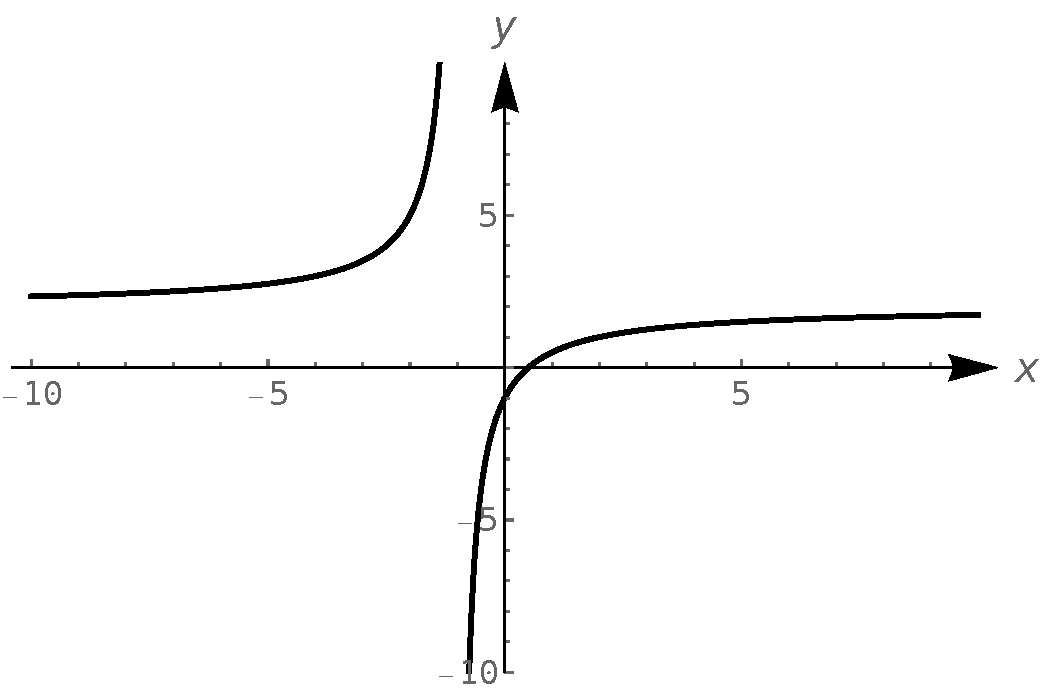
\includegraphics[width=0.5\textwidth]{fig_algebraic_8}
	\caption{The graph of $f(x)=\frac{2x-1}{x+1}$.}
	\label{fig_algebraic_8}
	\end{center}
\end{figure}

First, note that the graph appears to break at $x=-1$. We know from Example~\ref{ratfuncex} that $x=-1$ is not in the domain of $f$ which means $f(-1)$ is undefined. We see that we can get near $x=-1$ from two directions.  

% We can choose values a little less than $-1$, for example $x=-1.1$, $x=-1.01$, $x=-1.001$, and so on.  These values are said to approach $-1$ from the left.  Similarly, the values $x=-0.9$, $x=-0.99$, $x=-0.999$, etc., are said to approach $-1$ from the right.  If we make two tables, we find that the numerical results confirm what we see graphically.

% \renewcommand{\arraystretch}{1.5}
% \begin{center}
% \begin{tabular}{cc}

% $\begin{array}{r|c}  

%   x & f(x) \\ \hline\hline
%  -1.1 & 32 \\  
%  -1.01 & 302 \\  
%  -1.001 & 3002  \\  
%   -1.0001 & 30002  \\  
%   \end{array} $ \hspace{.75in} & 

% $\begin{array}{r|c}  
%   x & f(x)  \\ \hline\hline
%   -0.9 & -28  \\  
%   -0.99 & -298 \\  
%   -0.999 & -2998 \\  
%   -0.9999 & -29998 \\  

% \end{array}$

% \end{tabular}

% \end{center}
% \renewcommand{\arraystretch}{1}

As the $x$-values approach $-1$ from the left, the function values become larger and larger positive numbers. We express this symbolically by writing $x \underset{<}{\rightarrow} -1$, $f(x) \rightarrow +\infty$, or alternatively  $x \to -1^-$, \\ $f(x) \rightarrow +\infty$. Similarly, using analogous notation, we conclude  that as $x \underset{>}{\rightarrow} -1$, $f(x) \rightarrow -\infty$, or equivalently $x \to -1^+$, $f(x) \rightarrow -\infty$.  Here the $>$ means approaching from above and $<$ means approaching from below. For this type of unbounded behavior, we say the graph of $y=f(x)$ has a \index{asymptote ! vertical}\index{vertical asymptote}\index[aut]{ asymptoot  ! verticale}\index[aut]{verticale  asymptoot }\textbf{vertical asymptote} (\textit{verticale asymptoot}) of $x = -1$. 

The other feature worthy of note about the graph of $y=f(x)$ is that it seems to level off on the left and right hand sides of the plot window.  
% As $x$ attains larger  and larger negative values without bound,\ we may write $x \rightarrow -\infty$, while as $x$ becomes large without bound, we write $x \rightarrow +\infty$.  Making tables of values, we find
% \renewcommand{\arraystretch}{1.5}
% \begin{center}
% \begin{tabular}{cc}
% $\begin{array}{r|c}  
%   x & f(x)  \\ \hline\hline
%  -10 & \approx 2.3333  \\  
%  -100 & \approx 2.0303  \\  
%  -1000 &  \approx 2.0030  \\  
%   -10000 &  \approx 2.0003  \\  
%   \end{array} $ \hspace{.75in} & 
% $\begin{array}{r|c}  
%   x & f(x)  \\ \hline\hline
%  10 & \approx 1.7273 \\  
%  100 & \approx 1.9703 \\  
%  1000 &  \approx 1.9970 \\  
%   10000 &  \approx 1.9997 \\  
%   \end{array} $  \\
% \end{tabular}
% \end{center}
% \renewcommand{\arraystretch}{1}
We see that as $x \rightarrow -\infty$, $f(x)$ approaches 2 coming from values larger than 2 (from above) and as $x \rightarrow +\infty$, $f(x)$ approaches 2 though coming from values smaller than 2 (from below).   In this case, we say the graph of $y=f(x)$ has a \textbf{horizontal asymptote} (\textit{horizontale asymptoot}) of $y=2$.    We formalize the concepts of vertical and horizontal asymptotes in Chapter~\ref{chap_limits}.  We then also introduce the notion of a slant asymptote. \index{asymptote ! horizontal}\index{horizontal asymptote}\index[aut]{ asymptoot  ! horizontale}\index[aut]{horizontale  asymptoot }

\begin{example}
  A mathematical model for the population $P$ [--], in thousands, of a certain species of bacteria, $t$ [+] days after it is introduced to an environment is given by 
	$$P(t) = \frac{100}{(5-t)^{2}}\,,$$
for $0 \leq t < 5$.

\begin{enumerate}

\item  Find and interpret $P(0)$.

\item  When will the population reach $100\,000$?

\item  Determine the behavior of $P$ as $t \underset{<}{\rightarrow}  5$.  Interpret this result graphically and within the context of the problem. 

\end{enumerate}


\xhrulefill{gray}{2.5pt}Solution \xhrulefill{gray}{2.5pt}

\begin{enumerate}

\item  Substituting $t=0$ gives $P(0) = \frac{100}{(5-0)^2} = 4$, which means $4000$ bacteria are initially introduced into the environment.

\item   We remember that $P(t)$ is measured in thousands, so, $100\,000$ bacteria corresponds to $P(t) = 100$.  Substituting for $P(t)$ gives $$\frac{100}{(5-t)^2} = 100\,,$$
whose solution is $t = 4$ or $t=6$.  Of these two solutions, only $t=4$ lies in our domain, so this is the solution we keep.  Hence, it takes $4$ days for the population of bacteria to reach $100\,000$.

\item To determine the behaviour of $P$ as $t\underset{<}{\rightarrow} 5$, we can make a table

\renewcommand{\arraystretch}{1.25}
\[\begin{array}{r|c}  

  t & P(t)  \\ \hline\hline
 4.9 & 10\,000  \\  
 4.99 & 1000\,000  \\  
 4.999 &  100\,000\,000  \\  
  4.9999 & 10\,000\,000\,000  \\  
  \end{array}\]
  \renewcommand{\arraystretch}{1}

In other words, as $t \underset{<}{\rightarrow}\ 5$, $P(t) \rightarrow +\infty$.  The line $t=5$ is a vertical asymptote of the graph of $y=P(t)$.  This means that the population of bacteria is increasing without bound as we near 5 days, which cannot actually happen.  For this reason, $t=5$ is called the doomsday for this population. There is no way any environment can support infinitely many bacteria, so shortly before $t = 5$ the environment would collapse. 

\ifmathematica
In Mathematica, we can verify the correctness of our reasoning above by plotting the studied function using the built-in function \lstinline{Plot} as follows. 
\begin{mdframed}[default,backgroundcolor=gray!40,roundcorner=8pt]
\begin{mmaCell}[morefunctionlocal={t}]{Input}
  Plot[(100)/(5-t)^2,\{t,0,10\}]
\end{mmaCell}



\begin{mmaCell}[moregraphics={moreig={scale=.4}}]{Output}
	 \mmaGraphics{fig_algebraic_9}
\end{mmaCell}
\end{mdframed}

This plot becomes, however, more informative upon adding the axis labels and directions as follows. 
\begin{mdframed}[default,backgroundcolor=gray!40,roundcorner=8pt]
\begin{mmaCell}[morefunctionlocal={t}]{Input}
  Plot[(100)/(5-t)^2,\{t,0,10\}, 	AxesLabel ->\{"t (days)","P (-)"\},
	 AxesStyle->Arrowheads[\{0,0.05\}]]
\end{mmaCell}



\begin{mmaCell}[moregraphics={moreig={scale=.4}}]{Output}
	 \mmaGraphics{fig_algebraic_10}
\end{mmaCell}
\end{mdframed}
\fi

\ifpython
In Python, we can verify the correctness of our reasoning above by plotting the studied function using the built-in function \lstinline{plot} as follows. 

\begin{pyin}
from sympy import symbols
from sympy.plotting import plot
t = symbols('t')
plot((100)/(5-t)**2, xlim=(0,10), ylim=(0,250), xlabel="t (days)", ylabel="P (-)",
     adaptive=False, nb_of_points=1000)
\end{pyin}

\begin{pyout}
|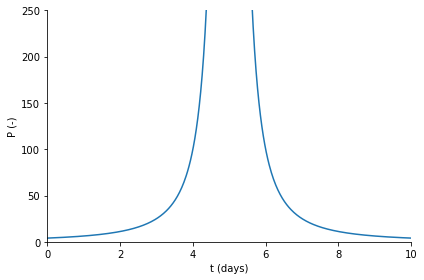
\includegraphics[width=0.5\textwidth]{fig_algebraic_10_Python.png}|
\end{pyout}
\fi
\end{enumerate}
\end{example}


\ifvc
We conclude this section with one example illustrating the practical use of rational functions. 




\begin{example}  \label{boxnotopfixedvolume} 
A box with a square base and no top is to be constructed so that it has a volume of $1000$ cubic centimetres.  Let $x$ [L] denote the width of the box, in centimetres as seen in Figure~\ref{fig_algebraic_11}.

\begin{figure}[H]
	\begin{center}
			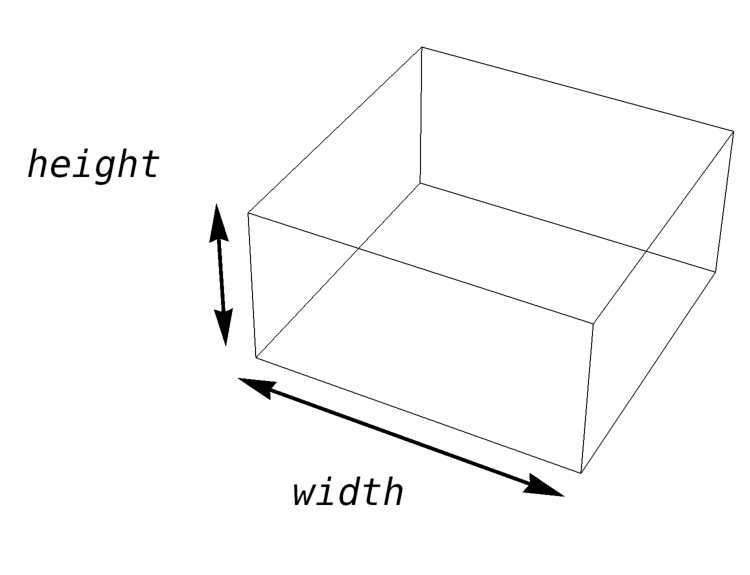
\includegraphics[width=0.5\textwidth]{fig_algebraic_11}
	\caption{Open box of width $x$ and height $h$.}
	\label{fig_algebraic_11}
	\end{center}
\end{figure}


\begin{enumerate}

\item  Express the height $h$ [L] in centimetres as a function of the width $x$ and state the applied domain.

\item  Solve $h(x) \geq x$ and interpret.

\item  Find and interpret the behaviour of $h(x)$ as $x \underset{>}{\rightarrow} 0$ and as $x \rightarrow +\infty$.

\item  Express the surface area $S$ of the box as a function of $x$ and state the applied domain.


\end{enumerate}

\xhrulefill{gray}{2.5pt}Solution \xhrulefill{gray}{2.5pt}

\begin{enumerate}

\item  We know that $\mbox{volume} = \mbox{width} \times \mbox{height} \times \mbox{depth}$.  Given that the base of the box is a square, the width and the depth are both $x$ centimetres.  Using $h$ for the height, we have $1000 = x^2h$, so that $h = 1000/x^2$.  Using function notation, $h(x) = \frac1000/x^2$.  As for the applied domain, in order for there to be a box at all, $x > 0$, and since every such choice of $x$ will return a positive number for the height $h$ we have no other restrictions and  conclude our domain is $\mathbb{R}^+_0$.

\item  To solve $h(x) \geq x$, we first collect all nonzero terms on one side of the inequality.

\[ \begin{array}{rrcl}

&h(x) & \geq & x  \\ [10pt]

\Leftrightarrow&\dfrac{1000}{x^2} & \geq & x \\ [10pt]

\Leftrightarrow&\dfrac{1000}{x^2} - x & \geq & 0 \\ [10pt]

\Leftrightarrow&\dfrac{1000-x^3}{x^2} & \geq & 0  \\[10pt]

\end{array} \]

We consider the left-hand side of the inequality as our rational function $r(x)$.  We see $r$ is undefined at $x=0$, but, the applied domain of the problem is $x > 0$, so we are considering only the behaviour of $r$ on $\left.\right]0, +\infty\left[\right.$.  The sole zero of $r$ comes when $1000-x^3 = 0$, which is $x=10$.  Choosing test values in the intervals $\left.\right]0,10\left[\right.$ and $\left.\right]10, +\infty\left[\right.$ allows to conclude that  $r(x) > 0$ on $\left.\right]0,10\left[\right.$, and since $r(x) = 0$ at $x=10$, our solution is $\left.\right]0,10]$.   Solving $h(x) \geq x$ is tantamount to find the values of $x$ which result in a box where the height is at least as big as the width (and, in this case, depth).  Our answer tells us the width of the box can be at most $10$ centimetres for this to happen.

\item As $x \underset{>}{\rightarrow} 0$, $h(x) \rightarrow +\infty$.  This means that the smaller the width $x$, the larger the height $h$ has to be in order to maintain a volume of $1000$ cubic centimetres. As $x \rightarrow +\infty$, we find $h(x) \underset{>}{\rightarrow}0$, which means that in order to maintain a volume of $1000$ cubic centimetres, the width and depth must get bigger as the height becomes smaller.

\item  Since the box has no top, the surface area can be found by adding the area of each of the sides to the area of the base.  The base is a square of dimensions $x$ by $x$, and each side has dimensions $x$ by $h$.  We get the surface area, $S = x^2+4xh$.  To get $S$ as a function of $x$, we substitute $h = 1000/x^2$ to obtain
$$S(x) = x^2 + \frac{4000}{x}.$$
The domain of $S$ is the same as $h$, namely $\mathbb{R}^+_0$.

\end{enumerate}
\end{example}
\fi


\ifanalysis
We conclude this section with one example illustrating the practical use of rational functions. 



\begin{example}
\label{ex_druk}
The actual data relating the volume $V$ [L$^3$] of a gas and its pressure $P$ [M L$^{-1}$T$^{-2}$] used by Boyle and his assistant in 1662 to verify the gas law that bears his name is given below.

\[ \begin{array}{c||c|c|c|c|c|c|c|c|c|c|c|c}  

V & 48 & 46 & 44 & 42 & 40 & 38 & 36 & 34 & 32 & 30 & 28 & 26   \\ \hline

P & 29.13 & 30.56 & 31.94 & 33.5 & 35.31 & 37 & 39.31 & 41.63 & 44.19 & 47.06 & 50.31 & 54.31 $\,$   \end{array} \]


\[\begin{array}{c||c|c|c|c|c|c|c|c|c|c|c} 

V & 24&23 & 22 & 21 & 20 & 19 & 18 & 17 & 16 & 15 & 14   \\ \hline 

P &58.81& 61.31 & 64.06 & 67.06 & 70.69 & 74.13 & 77.88 & 82.75 & 87.88 & 93.06 & 100.44   \end{array} \]


\[\begin{array}{c||c|c} 

V &  13 & 12  \\ \hline 

P &107.81 & 117.56   \end{array} \]

\begin{enumerate}
\ifmathematica
\item  Use Mathematica to create a scatter plot for these data using $V$ as the independent variable and $P$ as the dependent variable.  Does it appear from the graph that $P$ is inversely proportional to $V$?  Explain.

\item  Assuming that $P$ and $V$ do vary inversely, use the data to approximate the constant of proportionality.
\fi
\ifpython
\item  Use Python to create a scatter plot for these data using $V$ as the independent variable and $P$ as the dependent variable.  Does it appear from the graph that $P$ is inversely proportional to $V$?  Explain.

\item  Assuming that $P$ and $V$ do vary inversely, use the data to approximate the constant of proportionality.
\fi

\end{enumerate}


\xhrulefill{gray}{2.5pt}Solution \xhrulefill{gray}{2.5pt}

\begin{enumerate}
\ifmathematica
\item If $P$ really does vary inversely with $V$, then $P = \frac{k}{V}$ for some constant $k$.  To verify this, we create a scatterplot in Mathematica with the built-in function \lstinline{ListPlot} as follows. 

\begin{mdframed}[default,backgroundcolor=gray!40,roundcorner=8pt]
\begin{mmaCell}[moredefined={data,Arrowheads}]{Input}
  data=\{\{48,29.125`\},\{46,30.5625`\},\{44,31.9375`\},\{42,33.5`\},\{40,35.3125`\},
		\{38,37\},\{36,39.3125`\},\{34,41.625`\},\{32,44.1875`\},\{30,47.0625`\},
		\{28,50.3125`\},\{26,54.3125`\},\{24,58.8125`\},\{23,61.3125`\},\{22,64.0625`\},
		\{21,67.0625`\},\{20,70.6875`\},\{19,74.125`\},\{18,77.875`\},\{17,82.75`\},
		\{16,87.875`\},\{15,93.0625`\},\{14,100.4375`\},\{13,107.8125`\},\{12,117.5625`\}\};
		ListPlot[data,AxesLabel->\{"V","P"\},AxesStyle->Arrowheads[\{0,0.05`\}]]
\end{mmaCell}


\begin{mmaCell}[moregraphics={moreig={scale=.4}}]{Output}
	 \mmaGraphics{fig_algebraic_12}
\end{mmaCell}
\end{mdframed}

From the resulting plot, the points do seem to lie along a curve like $P = \frac{k}{V}$.

\item  To determine the constant of proportionality, we note that from $P = \frac{k}{V}$, we get $k = PV$.  Multiplying each of the volume numbers times each of the pressure numbers, we produce a number which is always approximately $1400$.  We suspect that $P = \frac{1400}{V}$.  Graphing this function  along with the data gives us good reason to believe our hypotheses that $P$ and $V$ are, in fact, inversely related. Again, we can do this in Mathematica using the built-in function \lstinline{Show} to combine multiple plots in one window. 

\begin{mdframed}[default,backgroundcolor=gray!40,roundcorner=8pt]
\begin{mmaCell}[moredefined={data,Arrowheads},morefunctionlocal={V}]{Input}
  Show[ListPlot[data,AxesLabel->\{"V","P"\},AxesStyle->Arrowheads[\{0,0.05`\}]],
		Plot[1400/V,\{V,0,50\}]]
\end{mmaCell}


\begin{mmaCell}[moregraphics={moreig={scale=.4}}]{Output}
	 \mmaGraphics{fig_algebraic_13}
\end{mmaCell}
\end{mdframed}
\fi

\ifpython
\item If $P$ really does vary inversely with $V$, then $P = \frac{k}{V}$ for some constant $k$.  To verify this, we create a scatterplot in Python with the built-in function \lstinline{scatter} as follows.
\begin{pyin}
import matplotlib.pyplot as plt
V = [48, 46, 44, 42, 40, 38, 36, 34, 32, 30, 28, 26, 24, 23, 22, 21, 20, 19, 18, 17,
    16, 15, 14, 13, 12]
P = [29.125, 30.5625, 31.9375, 33.5, 35.3125, 37, 39.3125, 41.625, 44.1875, 47.0625,
    50.3125, 54.3125, 58.8125, 61.3125, 64.0625, 67.0625, 70.6875, 74.125, 77.875,
    82.75, 87.875, 93.0625, 100.4375, 107.8125, 117.5625]
plt.scatter(V,P)
plt.xlabel('V')
plt.ylabel('P')
\end{pyin}
\begin{pyout}
|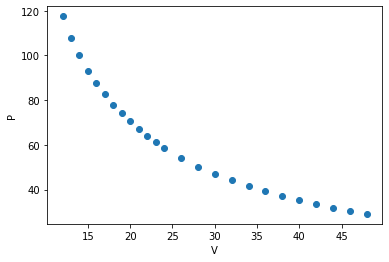
\includegraphics[width=0.5\textwidth]{fig_algebraic_12_Python}|
\end{pyout}

From the resulting plot, the points do seem to lie along a curve like $P = \frac{k}{V}$.

\item  To determine the constant of proportionality, we note that from $P = \frac{k}{V}$, we get $k = PV$.  Multiplying each of the volume numbers times each of the pressure numbers, we produce a number which is always approximately $1400$.  We suspect that $P = \frac{1400}{V}$.  Graphing this function  along with the data gives us good reason to believe our hypotheses that $P$ and $V$ are, in fact, inversely related. Again, we can do this in Python using the built-in function \lstinline{plot} to combine multiple plots in one window.
\begin{pyin}
import numpy as np
plt.scatter(V,P)
V = np.linspace(10, 50, 100)
P = 1400/V
plt.plot(V, P)
plt.xlabel('V')
plt.ylabel('P')
\end{pyin}
\begin{pyout}
|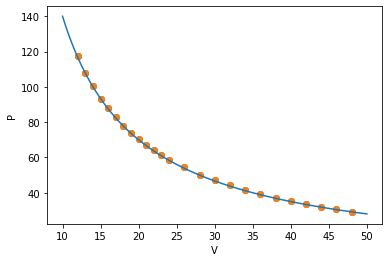
\includegraphics[width=0.5\textwidth]{fig_algebraic_13_Python}|
\end{pyout}
\fi

\end{enumerate}

\end{example}
\fi

\fi

\section{Irrational functions}
\label{irrat_functies}
This section serves as a watershed for functions which are combinations of polynomial, and more generally, rational functions, with the operations of radicals, such as
$$f(x) = \sqrt{1 - x^{2}}\,,$$
$$g(x) = \sqrt[4]{\dfrac{16x}{x^{2} - 9}}\,,$$
and
$$h(x) = \sqrt[3]{x^{3} + 3x^{2} - 6x - 8}\,.$$
\ifcourse
It is business of Part~\ref{deel2} to introduce the tools to better understand the behaviour of such functions in all the detail. Here we restrict to the basics to help shore up the requisite skills needed for a good understanding of the subsequent parts of this course. \fi In literature, functions containing radicals are sometimes referred to as \textbf{irrational functions} (\textit{irrationale functie}). \index{irrational function}\index[aut]{irrationale functie}

It is worth remarking that, in the light of Section~\ref{sec_inverse}, we could define $f(x) = \sqrt[n]{x}$ functionally as the inverse of $g(x) = x^n$ with the stipulation that when $n$ is even, the domain of $g$ is restricted to $\mathbb{R}^+$. From what we know about $g(x) = x^n$ from Section~\ref{sec_pol}, we can produce the graphs of $f(x) = \sqrt[n]{x}$ by reflecting the graphs of $g(x) = x^n$ across the line $y=x$.  Figures~\ref{fig_algebraic_14a}-\ref{fig_algebraic_14c} show the graphs of $y=\sqrt{x}$, $y=\sqrt[4]{x}$ and $y=\sqrt[6]{x}$ obtained in this way from the graphs of $y=x^2$, $y=x^4$ and $y=x^6$, respectively.  We can see the vertical steepening near $x=0$ and the horizontal flattening as $x \rightarrow +\infty$. Likewise, Figures~\ref{fig_algebraic_14d}-\ref{fig_algebraic_14f} show the graphs of $y=\sqrt[3]{x}$, $y=\sqrt[5]{x}$ and $y=\sqrt[7]{x}$ obtained by reflecting the graphs of $y=x^3$, $y=x^5$ and $y=x^7$ about the axis $y=x$, respectively. These odd-indexed radical functions also follow a predictable trend - steepening near $x = 0$ and flattening as $x \rightarrow \pm \infty$.



\begin{figure}
\centering
%\raisebox{0.5cm}{
\centerline{
\subfigure[\label{fig_algebraic_14a}]{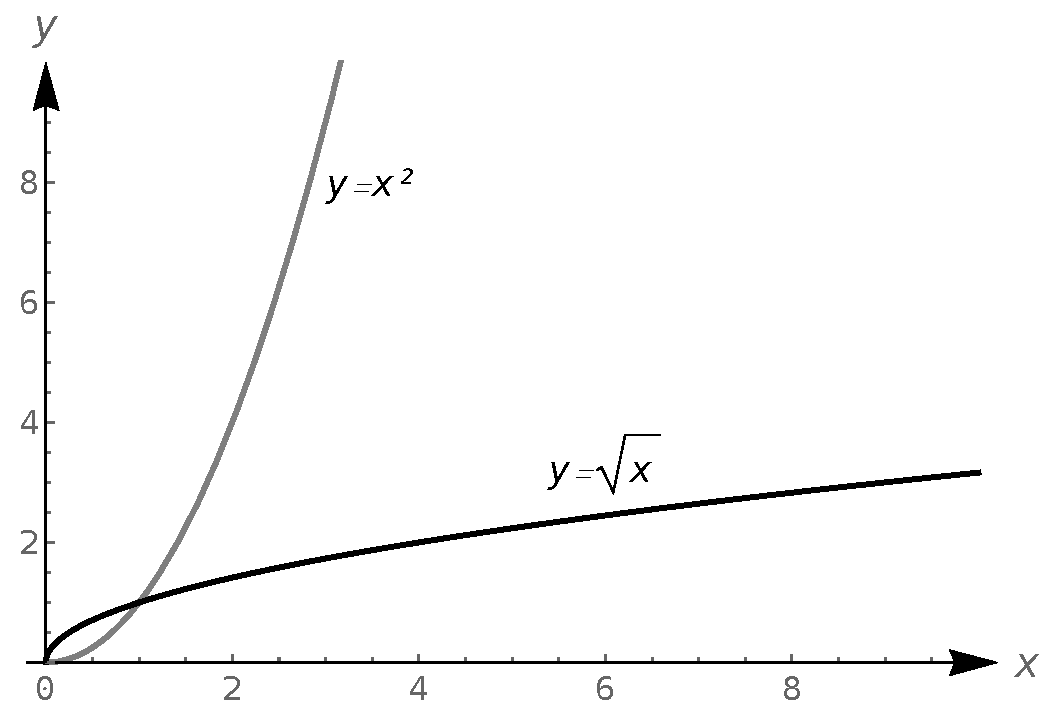
\includegraphics[width=0.3\textwidth]{fig_algebraic_14a}}
\hspace{0.1cm}
\subfigure[\label{fig_algebraic_14b}]{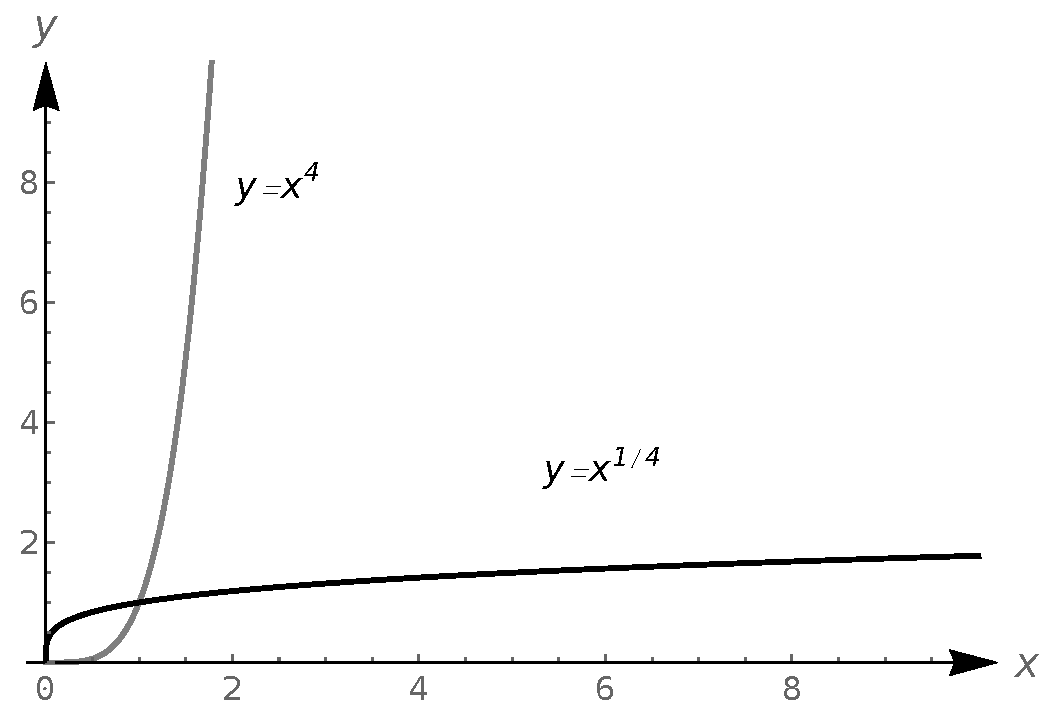
\includegraphics[width=0.3\textwidth]{fig_algebraic_14b}}
\hspace{0.1cm}
\subfigure[\label{fig_algebraic_14c}]{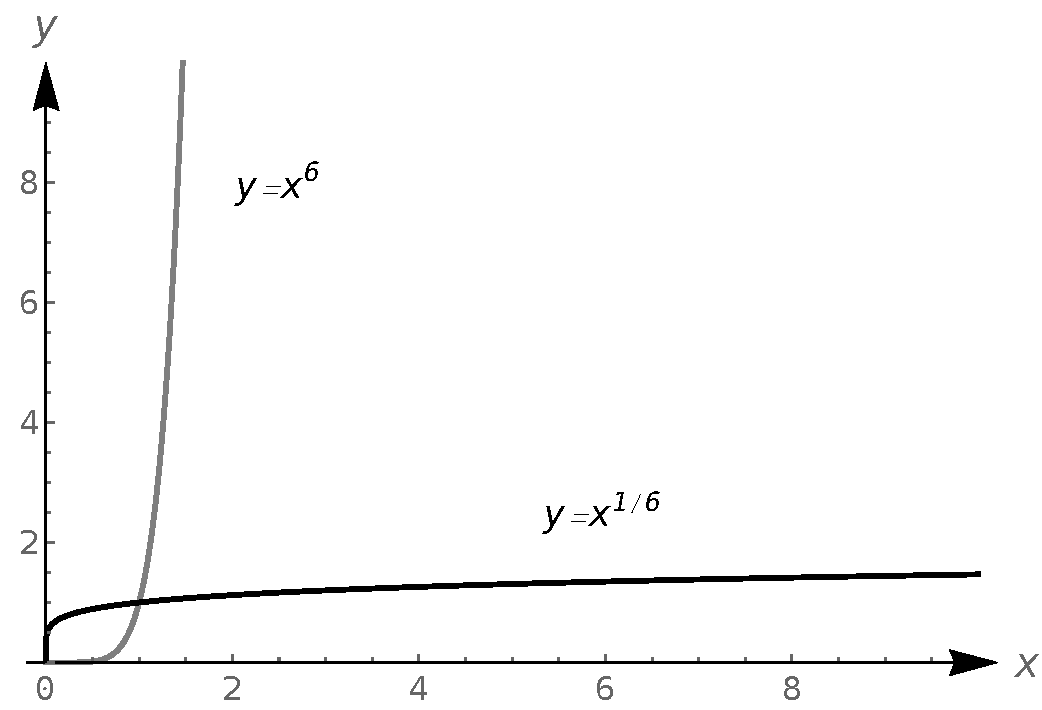
\includegraphics[width=0.3\textwidth]{fig_algebraic_14c}}
}
\centerline{
\subfigure[\label{fig_algebraic_14d}]{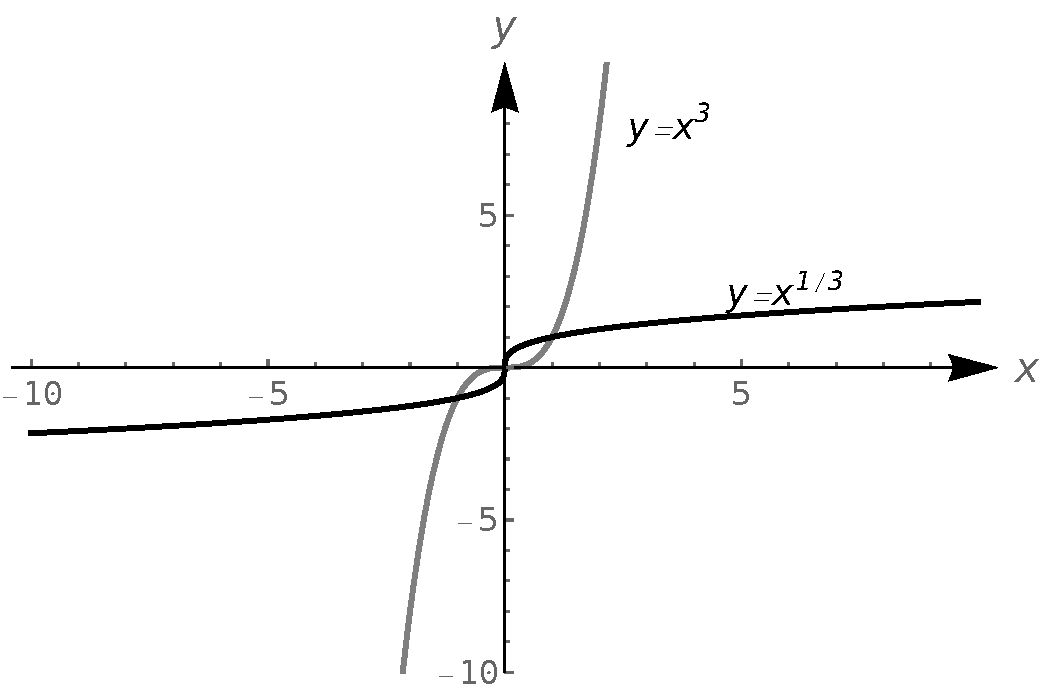
\includegraphics[width=0.3\textwidth]{fig_algebraic_14d}}
\hspace{0.1cm}
\subfigure[ \label{fig_algebraic_14e}]{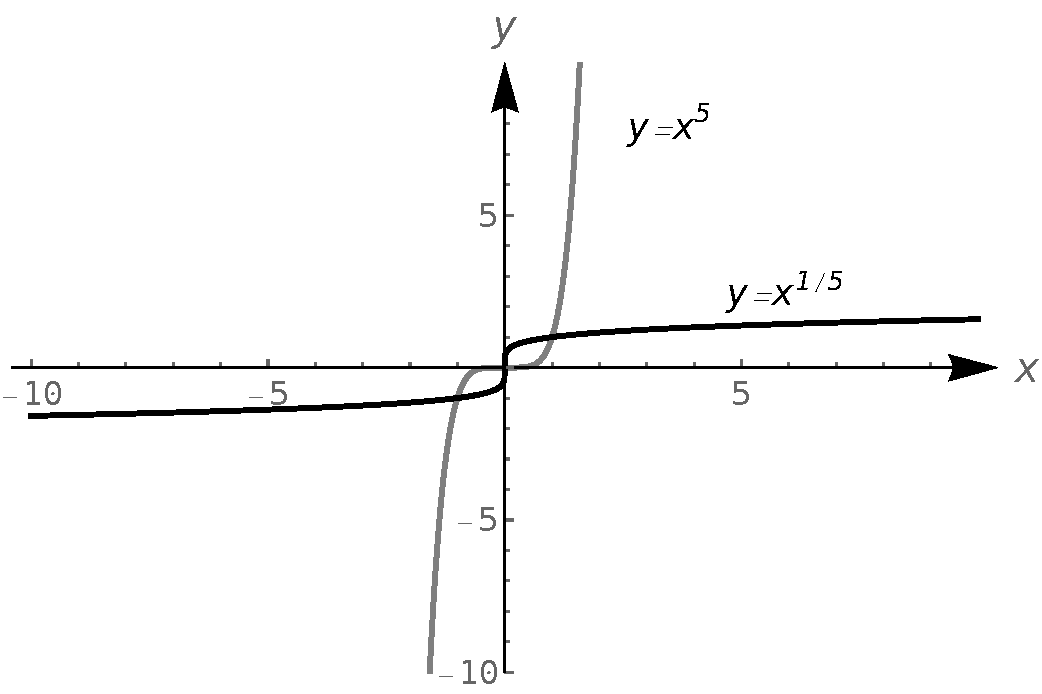
\includegraphics[width=0.3\textwidth]{fig_algebraic_14e}}
\hspace{0.1cm}
\subfigure[ \label{fig_algebraic_14f}]{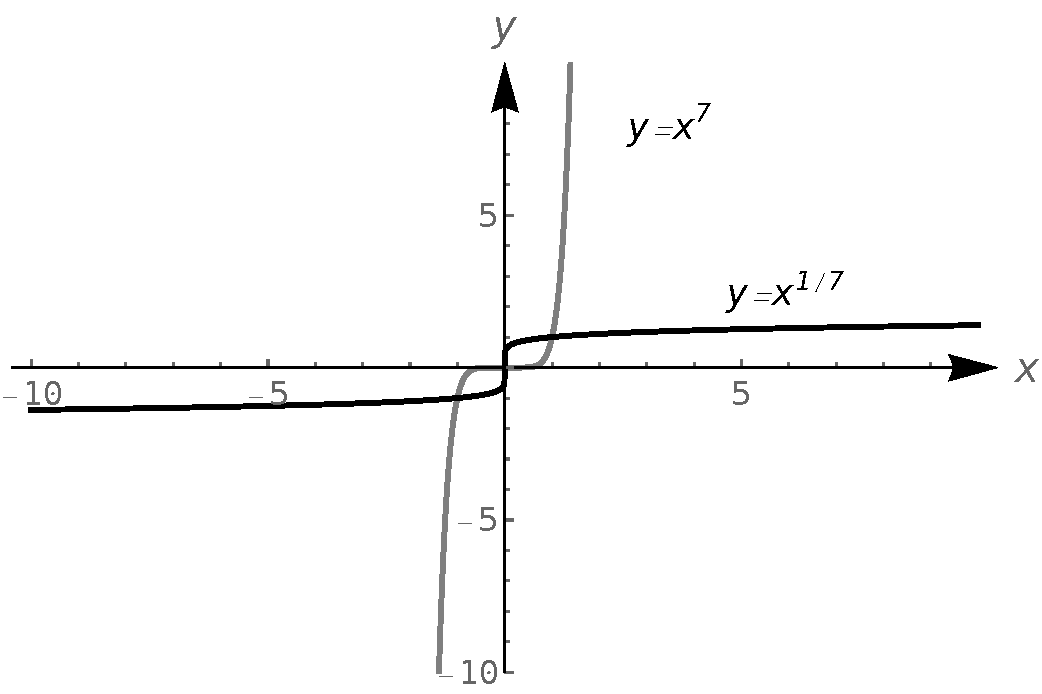
\includegraphics[width=0.3\textwidth]{fig_algebraic_14f}}
}
\caption{Graphs of  $y=\sqrt{x}$ (a), $y=\sqrt[4]{x}$ (b), $y=\sqrt[6]{x}$ (c), $y=\sqrt[3]{x}$ (d), $y=\sqrt[5]{x}$ (e) and $y=\sqrt[7]{x}$ (f). }
\end{figure}


\ifmathematica
\begin{example}  For the following functions, state their domains and determine their zero.  Check your answer graphically using Mathematica.

\begin{multicols}{2}
\begin{enumerate}

\item  $f(x) = 3x \sqrt[3]{2-x}$

\ifanalysis \item  $g(x) = \sqrt{2-\sqrt[4]{x+3}}$\fi


\ifvc\item  $h(x) = \sqrt[3]{\dfrac{8x}{x+1}}$\fi

\end{enumerate}
\end{multicols}

\xhrulefill{gray}{2.5pt}Solution \xhrulefill{gray}{2.5pt}



\begin{enumerate}

\item  As far as the domain is concerned, $f(x)$ has no denominators and no even roots, which means its domain is $\mathbb{R}$.  Its zeros can be found as follows.

\[ \begin{array}{rrclr}

&f(x) & = & 0 & \\

\Leftrightarrow&3x \sqrt[3]{2-x} & = & 0 \\

\Leftrightarrow&3x = 0 & \mbox{or} & \sqrt[3]{2-x} = 0 & \\

\Leftrightarrow&x = 0 & \mbox{or} & 2-x = 0 & \\

\Leftrightarrow&x = 0 & \mbox{or} & x=2 & \\

\end{array}\]


The zeros $0$ and $2$ divide the real number line into three intervals, where the function may have a different behaviour. The graph of this function is shown in Figure~\ref{fig_algebraic_15}.
\begin{figure}[H]
    \begin{center}
			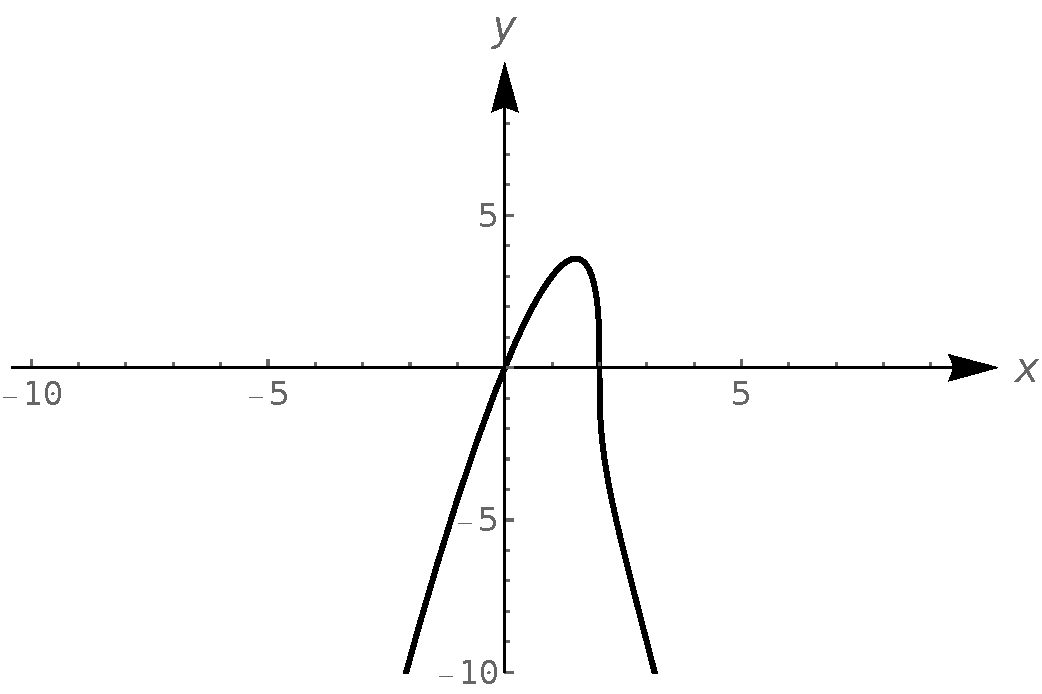
\includegraphics[width=0.5\textwidth]{fig_algebraic_15}
	\end{center}
    \caption{Graph of $f(x) = 3x \sqrt[3]{2-x}$.}
    \label{fig_algebraic_15}
\end{figure}
  
  
\ifcourse 	
\ifanalysis
\item In $g(x) = \sqrt{2-\sqrt[4]{x+3}}$, we have two radicals both of which are even indexed.  To satisfy $\sqrt[4]{x+3}$, we require $x+3 \geq 0$ or $x \geq -3$.  To satisfy $ \sqrt{2-\sqrt[4]{x+3}}$, we need $2-\sqrt[4]{x+3} \geq 0$.  Hence, we solve $2-\sqrt[4]{x+3} \geq 0$.  If we let $r(x) = 2-\sqrt[4]{x+3}$, we know $x \geq -3$, so we  concern ourselves with only this portion of the number line.  To find the zeros of $r$ we set $r(x) =0$ and solve  $2-\sqrt[4]{x+3}=0$:
$$
2-\sqrt[4]{x+3}=0\quad\Leftrightarrow \quad\sqrt[4]{x+3}=2\,,
$$
which implies that $x+3=2^4=16$, so $x=13$.
  Since we raised both sides of an equation to an even power, we need to check to see if $x=13$ is an extraneous solution.  We find $x=13$ does check since $2-\sqrt[4]{x+3} = 2 - \sqrt[4]{13+3} = 2 - \sqrt[4]{16} = 2 - 2 = 0$. We find $2-\sqrt[4]{x+3} \geq 0$ on $[-3,13]$ so this is the domain of $g$. 
For what concerns $g$, we look for its zeros.  Setting $g(x) = 0$ is equivalent to $\sqrt{2-\sqrt[4]{x+3}}=0$.  After squaring both sides, we get $2-\sqrt[4]{x+3} = 0$, whose solution we have found to be $x=13$.   Since we squared both sides, we double check and find $g(13)$ is, in fact, $0$. The domain of $g$ is $[-3,13]$. This graph of this function is shown in Figure~\ref{fig_algebraic_16}.
\begin{figure}[H]
    \begin{center}
			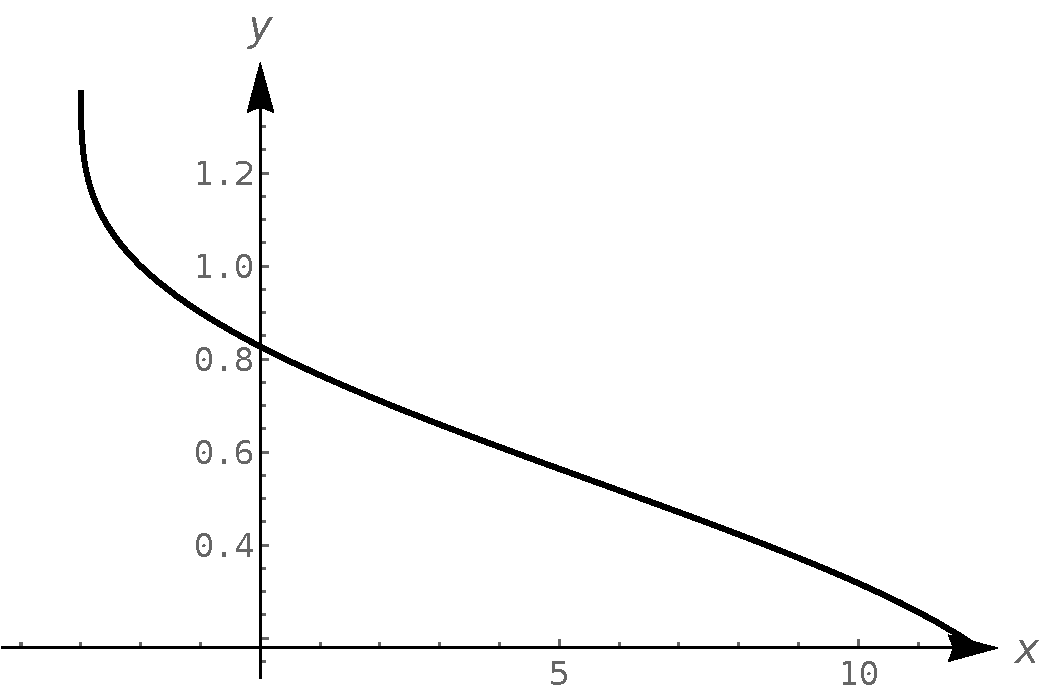
\includegraphics[width=0.45\textwidth]{fig_algebraic_16}
	\end{center}
    \caption{Graph of $g(x) = \sqrt{2-\sqrt[4]{x+3}}$.}
    \label{fig_algebraic_16}
\end{figure}
\fi
\fi

\ifvc
\item  The radical in $h(x)$ is odd, so our only concern is the denominator.  Setting $x+1=0$ gives $x=-1$, so our domain is $\mathbb{R}\setminus\{-1\}$.  To find the zeros of $h$, we set $h(x) = 0$ and solve for $x$:
$$
\sqrt[3]{\frac{8x}{x+1}} = 0\quad\Leftrightarrow\quad\frac{8x}{x+1} = 0\,.
$$
  We get $x=0$. From the graph, depicted in Figure~\ref{fig_algebraic_17}, it appears as though $x=-1$ is a vertical asymptote.
\begin{figure}[H]
    \begin{center}
			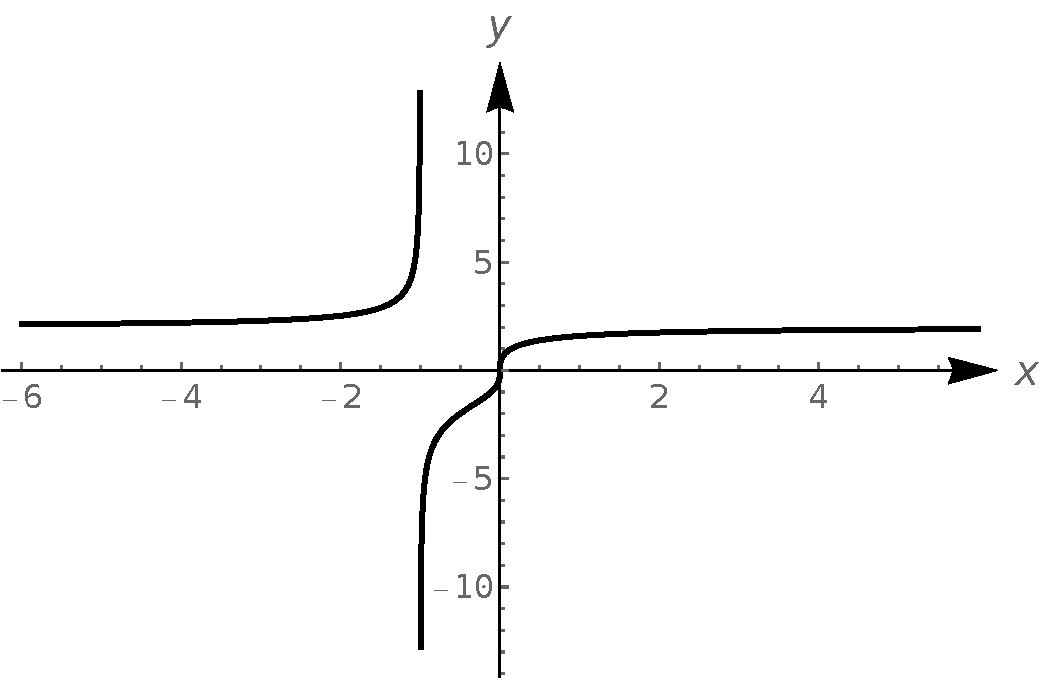
\includegraphics[width=0.5\textwidth]{fig_algebraic_17}
	\end{center}
    \caption{Graph of $h(x) = \sqrt[3]{\frac{8x}{x+1}}$.}
    \label{fig_algebraic_17}
\end{figure}
\fi 

\end{enumerate}
\end{example}
\fi

\ifpython
\begin{example}  For the following functions, state their domains and determine their zero.  Check your answer graphically using Python.

\begin{multicols}{2}
\begin{enumerate}

\item  $f(x) = 3x \sqrt[3]{2-x}$

\ifanalysis \item  $g(x) = \sqrt{2-\sqrt[4]{x+3}}$\fi


\ifvc\item  $h(x) = \sqrt[3]{\dfrac{8x}{x+1}}$\fi

\end{enumerate}
\end{multicols}

\xhrulefill{gray}{2.5pt}Solution \xhrulefill{gray}{2.5pt}



\begin{enumerate}

\item  As far as the domain is concerned, $f(x)$ has no denominators and no even roots, which means its domain is $\mathbb{R}$.  Its zeros can be found as follows.

\[ \begin{array}{rrclr}

&f(x) & = & 0 & \\

\Leftrightarrow&3x \sqrt[3]{2-x} & = & 0 \\

\Leftrightarrow&3x = 0 & \mbox{or} & \sqrt[3]{2-x} = 0 & \\

\Leftrightarrow&x = 0 & \mbox{or} & 2-x = 0 & \\

\Leftrightarrow&x = 0 & \mbox{or} & x=2 & \\

\end{array}\]


The zeros $0$ and $2$ divide the real number line into three intervals, where the function may have a different behaviour. The graph of this function is shown in Figure~\ref{fig_algebraic_15}.
\begin{figure}[H]
    \begin{center}
			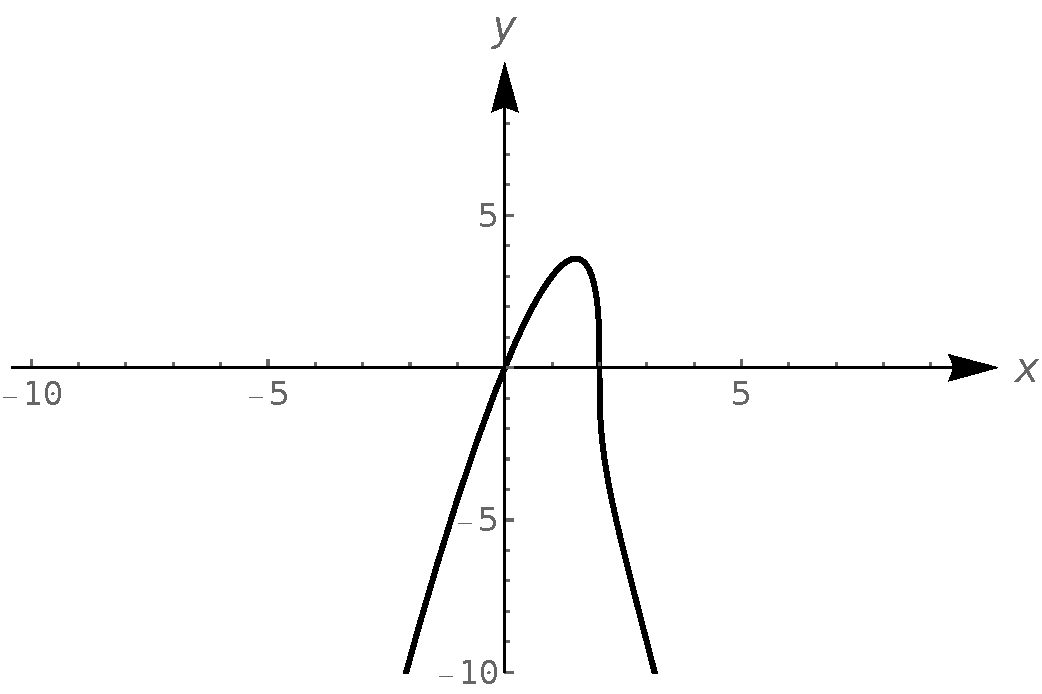
\includegraphics[width=0.5\textwidth]{fig_algebraic_15}
	\end{center}
    \caption{Graph of $f(x) = 3x \sqrt[3]{2-x}$.}
    \label{fig_algebraic_15}
\end{figure}
  
  
\ifcourse 	
\ifanalysis
\item In $g(x) = \sqrt{2-\sqrt[4]{x+3}}$, we have two radicals both of which are even indexed.  To satisfy $\sqrt[4]{x+3}$, we require $x+3 \geq 0$ or $x \geq -3$.  To satisfy $ \sqrt{2-\sqrt[4]{x+3}}$, we need $2-\sqrt[4]{x+3} \geq 0$.  Hence, we solve $2-\sqrt[4]{x+3} \geq 0$.  If we let $r(x) = 2-\sqrt[4]{x+3}$, we know $x \geq -3$, so we  concern ourselves with only this portion of the number line.  To find the zeros of $r$ we set $r(x) =0$ and solve  $2-\sqrt[4]{x+3}=0$:
$$
2-\sqrt[4]{x+3}=0\quad\Leftrightarrow \quad\sqrt[4]{x+3}=2\,,
$$
which implies that $x+3=2^4=16$, so $x=13$.
  Since we raised both sides of an equation to an even power, we need to check to see if $x=13$ is an extraneous solution.  We find $x=13$ does check since $2-\sqrt[4]{x+3} = 2 - \sqrt[4]{13+3} = 2 - \sqrt[4]{16} = 2 - 2 = 0$. We find $2-\sqrt[4]{x+3} \geq 0$ on $[-3,13]$ so this is the domain of $g$. 
For what concerns $g$, we look for its zeros.  Setting $g(x) = 0$ is equivalent to $\sqrt{2-\sqrt[4]{x+3}}=0$.  After squaring both sides, we get $2-\sqrt[4]{x+3} = 0$, whose solution we have found to be $x=13$.   Since we squared both sides, we double check and find $g(13)$ is, in fact, $0$. The domain of $g$ is $[-3,13]$. This graph of this function is shown in Figure~\ref{fig_algebraic_16}.
\begin{figure}[H]
    \begin{center}
			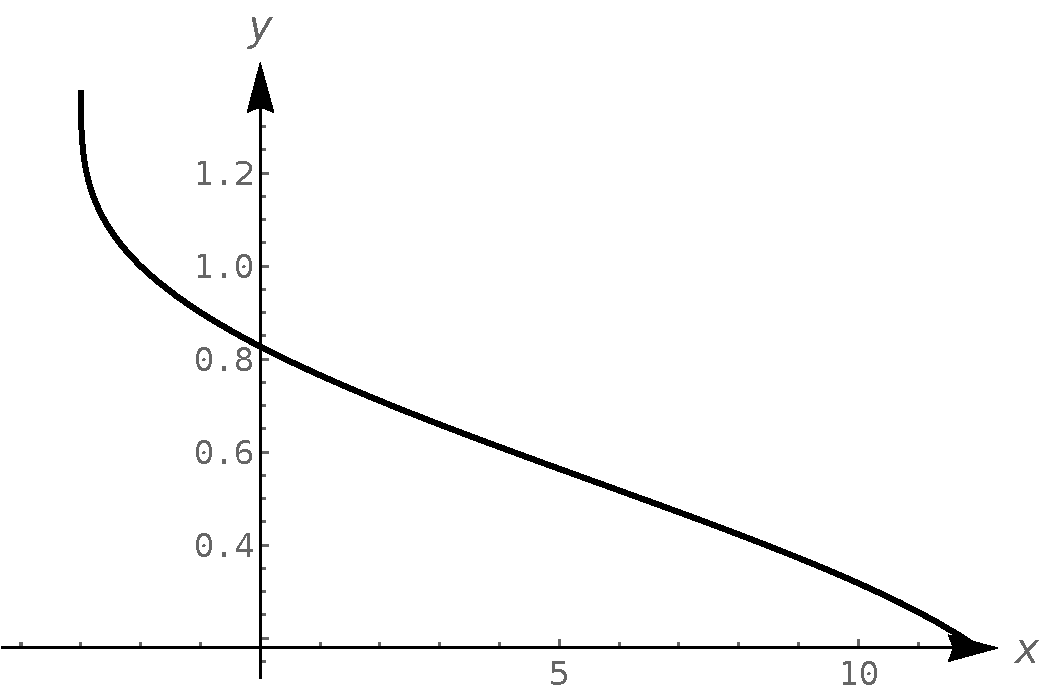
\includegraphics[width=0.45\textwidth]{fig_algebraic_16}
	\end{center}
    \caption{Graph of $g(x) = \sqrt{2-\sqrt[4]{x+3}}$.}
    \label{fig_algebraic_16}
\end{figure}
\fi
\fi

\ifvc
\item  The radical in $h(x)$ is odd, so our only concern is the denominator.  Setting $x+1=0$ gives $x=-1$, so our domain is $\mathbb{R}\setminus\{-1\}$.  To find the zeros of $h$, we set $h(x) = 0$ and solve for $x$:
$$
\sqrt[3]{\frac{8x}{x+1}} = 0\quad\Leftrightarrow\quad\frac{8x}{x+1} = 0\,.
$$
  We get $x=0$. From the graph, depicted in Figure~\ref{fig_algebraic_17}, it appears as though $x=-1$ is a vertical asymptote.
\begin{figure}[H]
    \begin{center}
			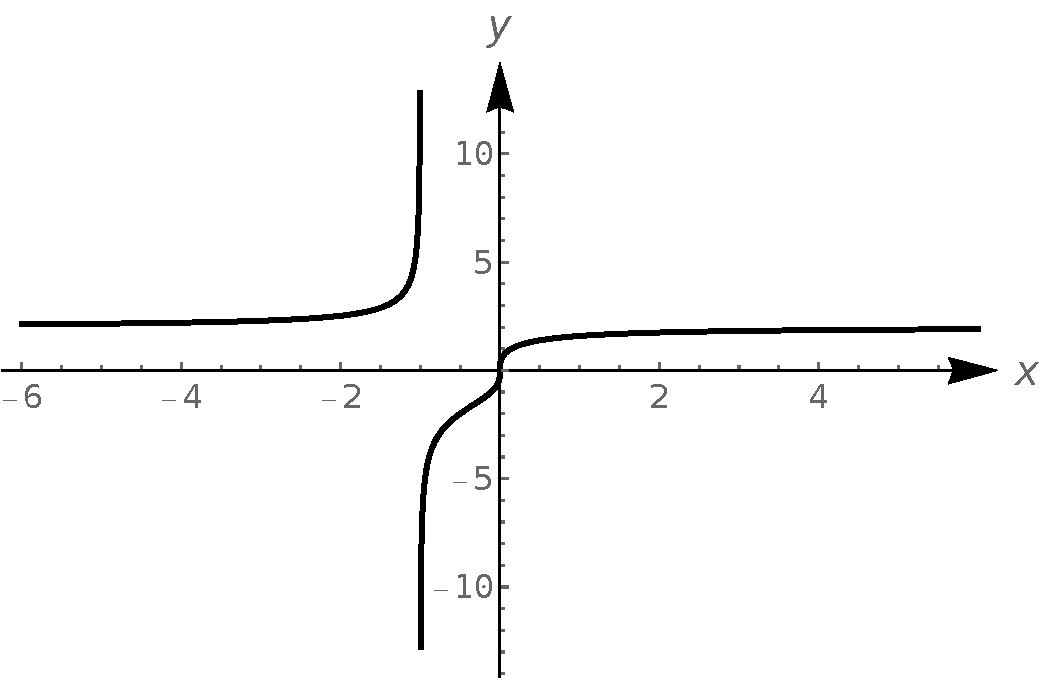
\includegraphics[width=0.5\textwidth]{fig_algebraic_17}
	\end{center}
    \caption{Graph of $h(x) = \sqrt[3]{\frac{8x}{x+1}}$.}
    \label{fig_algebraic_17}
\end{figure}
\fi 

\end{enumerate}
\end{example}
\fi



\ifcourse
We conclude this section with an application in which an irrational function pops up naturally. 

\begin{example}
 \label{SasquatchCable} Carl wishes to get high speed internet service installed in his remote bird observation post located $30$ metres from the E34. The nearest junction box is located $50$ metres downroad  (Figure~\ref{fig_algebraic_18}).  Suppose it costs $\text{\euro} 15$ per metre to run cable along the road and $\text{\euro} 20$ per metre to run cable off of the road.

Express the total cost $C$ of connecting the Junction Box to the Outpost as a function of $x$, the number of metres the cable is run along the E34 before heading off road directly towards the Outpost.  Determine a reasonable applied domain for the problem.

\begin{figure}[H]
    \begin{center}
			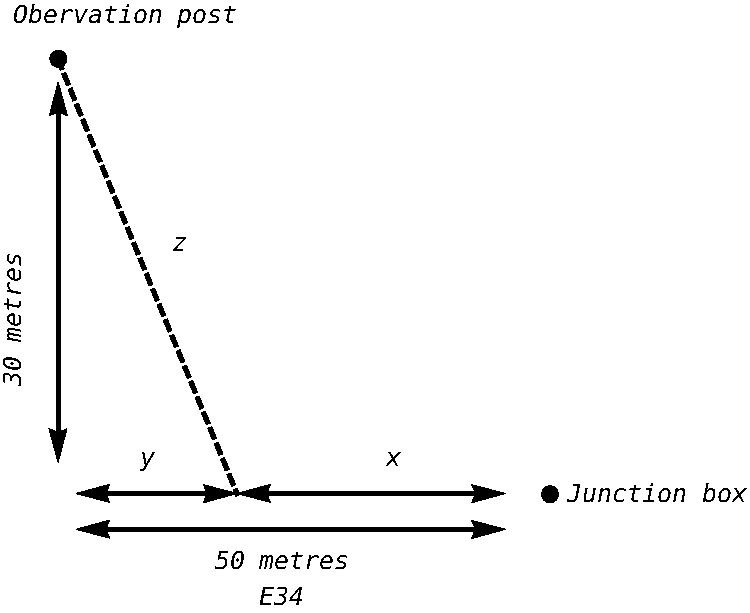
\includegraphics[width=0.4\textwidth]{fig_algebraic_18}
	\end{center}
    \caption{Map showing the observation post and junction box in Example~\ref{SasquatchCable}.}
    \label{fig_algebraic_18}
\end{figure}

\ifcalculus\pagebreak\fi
\xhrulefill{gray}{2.5pt}Solution \xhrulefill{gray}{2.5pt}

 The cost is broken into two parts:  the cost to run cable along the E34 at $\text{\euro} 15$ per metre, and the cost to run it off road at $\text{\euro} 20$ per metre.  Since $x$ represents the metres of cable run along the E34, the cost  for that portion is $15x$.  From Figure~\ref{fig_algebraic_18}, we see that the number of metres the cable is run off road is $z$, so the cost of that portion is $20z$.

 Hence, the total cost is $C = 15x + 20z$.  Our next goal is to determine $z$ as a function of $x$.  The diagram suggests we can use the Pythagorean theorem to get $y^2+30^2 = z^2$.  But we also see $x+y = 50$ so that $y=50-x$.  Hence, $z^2 = (50-x)^2+900$.  Solving for $z$, we obtain $z = \pm \sqrt{(50-x)^2+900}$.  Since $z$ represents a distance, we choose $z = \sqrt{(50-x)^2+900}$ so that our cost as a function of $x$ only is given by \[C(x) = 15x + 20\sqrt{(50-x)^2+900}\,.\] From the context of the problem, we have $0 \leq x \leq 50$.

\end{example}

\fi


\pagebreak
\section{Conic sections}
\label{sec_conic}
In this section, we will investigate the two-dimensional figures that are formed when a right circular cone is intersected by a plane.

\ifcourse
\begin{remark}[History of conic sections]
The Greek mathematician Menaechmus (c. 380-c. 320 BCE) is generally credited with discovering the shapes formed by the intersection of a plane and a right circular cone. Depending on how he tilted the plane when it intersected the cone, he formed different shapes at the intersection -- beautiful shapes with near-perfect symmetry. It was also said that Aristotle may have had an intuitive understanding of these shapes, as he observed the orbit of the planet to be circular. He presumed that the planets moved in circular orbits around Earth, and for nearly 2000 years this was the commonly held belief.

It was not until the Renaissance movement that Johannes Kepler noticed that the orbits of the planet were not circular in nature. His law of planetary motion in the 1600s changed our view of the solar system forever. He claimed that the sun was at one end of the orbits, and the planets revolved around the sun in an oval-shaped path.
\end{remark}
\fi


\subsection{Overview}

The name \textbf{conic section} (\textit{kegelsnede}) is used to refer to any of the shapes that can be formed by intersecting a double-napped right circular cone with a plane. There are indeed several ways to intersect such a cone by a plane. Let us first consider a plane that does not contain the cone's vertex. Then, we can slice its top nappe, for instance, with a horizontal plane. This produces a circle (Figure~\ref{fig_algebraic_19a}). Tilting this plane only slightly produces an ellipse (Figure~\ref{fig_algebraic_19b}), while tilting the plane even further leads to a parabola (Figure~\ref{fig_algebraic_19c}). If we continue increasing the tilting angle like this, the plane will at some point cut through both nappes, giving rise to a hyperbola (Figure~\ref{fig_algebraic_19d}). 


\index{conic section} \index[aut]{kegelsnede}

\begin{figure}[t]
\centering
%\raisebox{0.5cm}{
\centerline{
\subfigure[\label{fig_algebraic_19a}]{
\includegraphics[width=0.4\textwidth]{fig_algebraic_19a}}
\hspace{0.1cm}
\subfigure[ \label{fig_algebraic_19b}]{
\includegraphics[width=0.4\textwidth]{fig_algebraic_19b}}
}
\centerline{
\subfigure[\label{fig_algebraic_19c}]{
\includegraphics[width=0.4\textwidth]{fig_algebraic_19c}}
\hspace{0.1cm}
\subfigure[ \label{fig_algebraic_19d}]{
\includegraphics[width=0.4\textwidth]{fig_algebraic_19d}}
}
\caption{The intersection of a double-napped right circular cone with a plane with varying tilting angle: a circle (a), ellipse (b), parabola (c) and hyperbola (d). }
\end{figure}

If the slicing plane contains the vertex of the cone, we get the so-called degenerate conics, namely a point (Figure~\ref{fig_algebraic_20a}), a line (Figure~\ref{fig_algebraic_20b}) or two intersecting lines (Figure~\ref{fig_algebraic_20c}). 

\begin{figure}[h]
\centering
%\raisebox{0.5cm}{
\centerline{
\subfigure[\label{fig_algebraic_20a}]{
\includegraphics[width=0.4\textwidth]{fig_algebraic_20a}}
\hspace{0.1cm}
\subfigure[ \label{fig_algebraic_20b}]{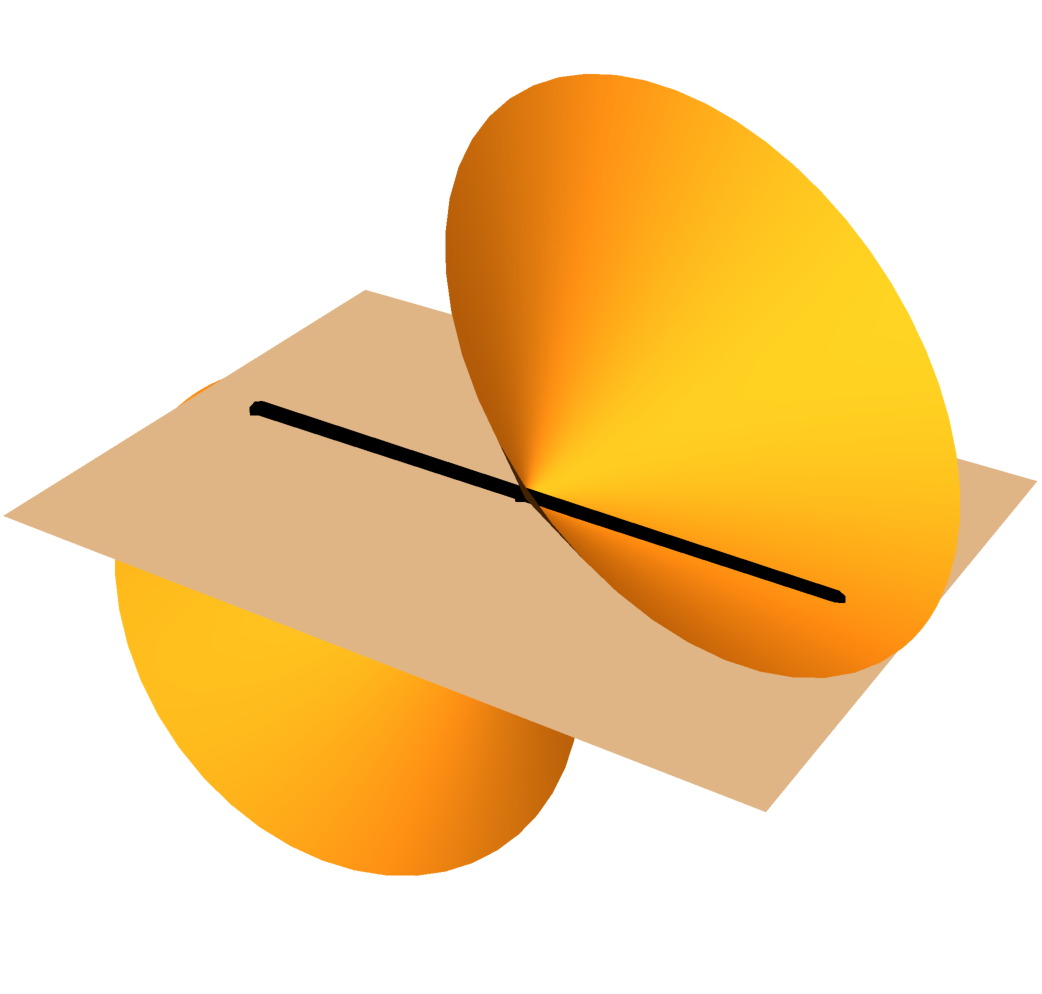
\includegraphics[width=0.4\textwidth]{fig_algebraic_20b}}
}
\centerline{
\subfigure[\label{fig_algebraic_20c}]{
\includegraphics[width=0.4\textwidth]{fig_algebraic_20c}}
}
\caption{The intersection of a double-napped right circular cone with a plane containing the vertex of the cone and with varying tilting angle: a point (a), line (b) and two intersecting lines (c). }
\end{figure}

In the remainder of this section we will review the non-degenerate cases in detail. \ifcourse Then, in Chapter~\ref{chap_trans}  we will show how any quadratic equation of the form
$$
ax^2+bxy+cy^2+dx+ey+f=0
$$
corresponds to a conic section.  \fi


\subsection{Circles}
In geometry, a circle is defined as follows. \index{radius}\index{centre}\index[aut]{straal}\index[aut]{middelpunt}


\begin{definition}[Circle] \label{circledefn}
 A \textbf{circle} (\textit{cirkel}) with \textbf{centre} (\textit{middelpunt}) $(x_0,y_0)$ and \textbf{radius} (\textit{straal}) $r>0$ is the set of all points $(x, y)$ in the plane whose distance to $(x_0,y_0)$ is $r$.
 \index[aut]{cirkel} \index[aut]{middelpunt} \index[aut]{straal}
 \index{circle} \index{centre} \index{radius}
\end{definition} 

We  express this definition algebraically using the distance formula as 
\[r = \sqrt{(x - x_0)^2 + (y-y_0)^2}\,.\] 

By squaring both sides of this equation, we get an equivalent equation (since $r > 0$) which gives us the standard equation of a circle with centre $(x_0,y_0)$ and radius $r$:
\begin{equation}
\label{standardcircle}
(x-x_0)^2 + (y-y_0)^2 = r^2.
\end{equation}

%\begin{example}  
%Graph the circle 
%$$(x+2)^2+(y-1)^2 = 4, $$ 
%and find its centre and radius.

%\xhrulefill{gray}{2.5pt}Solution \xhrulefill{gray}{2.5pt}

% From the standard form of a circle, Equation \eqref{standardcircle}, we have that $x + 2$ is  $x-x_0$, so $x_0 = -2$ and $y - 1$ is $y - y_0$ so $y_0 = 1$.  This tells us that our centre is $(-2,1)$.  Furthermore, $r^2 = 4$, so $r = 2$. Thus we have a circle centred at $(-2,1)$ with a radius of $2$.  The resulting graph is presented in Figure~\ref{fig_algebraic_16}.
 %\begin{figure}[H]
  %   \begin{center}
%			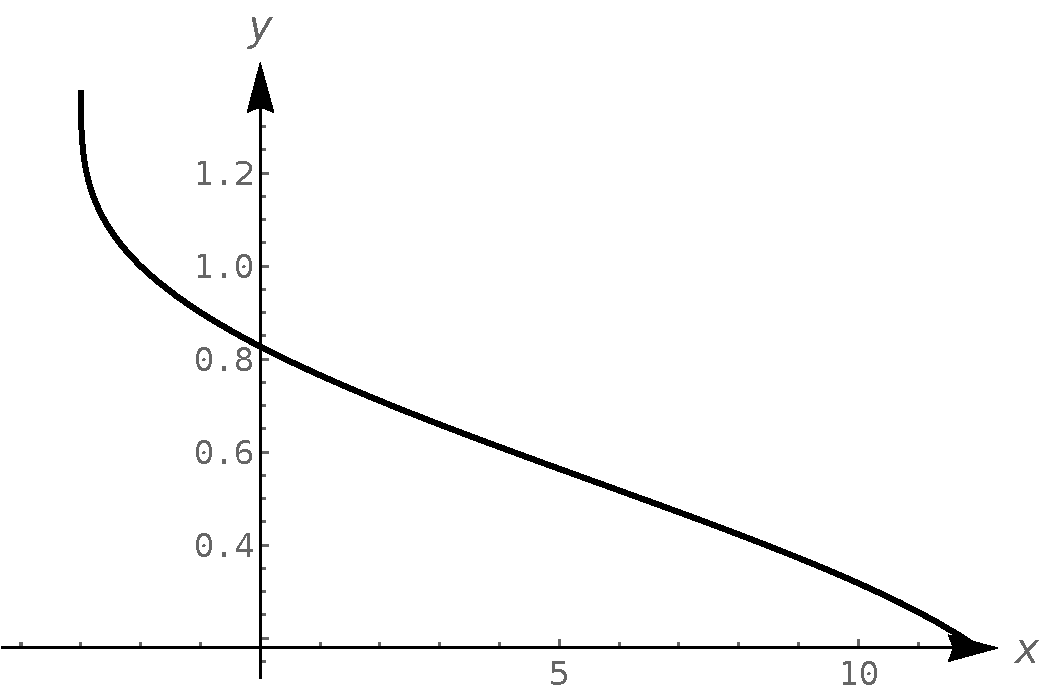
\includegraphics[width=0.5\textwidth]{fig_algebraic_16}
%	\end{center}
 %    \caption{Graph of the circle $(x+2)^2+(y-1)^2 = 4$.}
  %   \label{fig_algebraic_16}
 %\end{figure}
  	
%\end{example}

%If we were to expand the equation in the previous example and gather up like terms, instead of the easily recognizable $(x+2)^2 + (y-1)^2 = 4$, we would be contending with $x^2 + 4x + y^2 - 2y  + 1 = 0.$  If we're given such an equation, we can complete the square in each of the variables to see if it fits the form given in Equation~\eqref{standardcircle}.

\ifvc
\begin{example}  Write the standard equation of the circle which has $(-1,3)$ and $(2,4)$ as the endpoints of a diameter.

\xhrulefill{gray}{2.5pt}Solution \xhrulefill{gray}{2.5pt}

 Since the given points are endpoints of a diameter, we know their midpoint $(x_0, y_0)$ is the centre of the circle.  Hence,

\[ \begin{array}{rcl} (x_0,y_0) &  = & \left( \dfrac{x_1 + x_2}{2},  \dfrac{y_1 + y_2}{2} \right) \\ [8pt]
&  = &  \left( \dfrac{-1+2}{2},  \dfrac{3+4}{2} \right) \\ [8pt]
& = &  \left( \dfrac{1}{2},  \dfrac{7}{2} \right)  \end{array} \]

The diameter of the circle is the distance between the given points, so we know that half of the distance is the radius.  Thus, 

\[ \begin{array}{rcl} r &  = & \dfrac{1}{2} \sqrt{\left(x_2 - x_1\right)^2+\left(y_2-y_1\right)^2}  \\ [8pt]
 &  = & \dfrac{1}{2} \sqrt{(2-(-1))^2+(4-3)^2} \\ [8pt]
 & = &\dfrac{\sqrt{10}}{2}. \end{array} \]

Finally, since $\left( \frac{\sqrt{10}}{2} \right)^2 = \frac{10}{4}$, our answer becomes 
$$\left(x - \dfrac{1}{2} \right)^2 + \left(y - \dfrac{7}{2} \right)^2 =\dfrac{10}{4}.$$ 

\end{example}
\fi

We close our introduction to circles with the most important circle in all of mathematics:  the unit circle.

\begin{definition}[Unit circle]

The \textbf{unit circle} (\textit{eenheidscirkel})\index{unit circle}\index[aut]{eenheidscirkel}\label{UnitCircle} is the circle centred at $(0,0)$ with a radius of $1$.  The standard equation of the unit circle is 
$$x^2 + y^2 = 1.$$

\end{definition}

\ifanalysis\pagebreak\fi
\subsection{Ellipses}
In the definition of a circle, (Definition~\ref{circledefn}), we fixed a point called the centre and considered all of the points which were at a fixed distance $r$ from that one point.  For the ellipse, we fix two distinct points and a distance $d$.  

 \begin{definition}[Ellipse] 
\label{ellipsedefn} 
Given two distinct points $F_1$ and $F_2$ in the plane and a fixed distance $d$, an \textbf{ellipse} (\textit{ellips}) is the set of all points $(x, y)$ in the plane such that the sum of each of the distances from $F_1$ and $F_2$ to $(x, y)$ is $d$.  The points $F_1$ and $F_2$   are called the \textbf{foci} (\textit{brandpunten}) of the ellipse. \index{ellipse ! focus}\index[aut]{ellips ! brandpunt}
\end{definition} 
We may imagine taking a length of string and anchoring it to two points on a piece of paper.  The curve traced out by taking a pencil and moving it so the string is always taut is an ellipse (Figure~\ref{fig_algebraic_21}). 

\begin{figure}[h]
	\begin{center}
			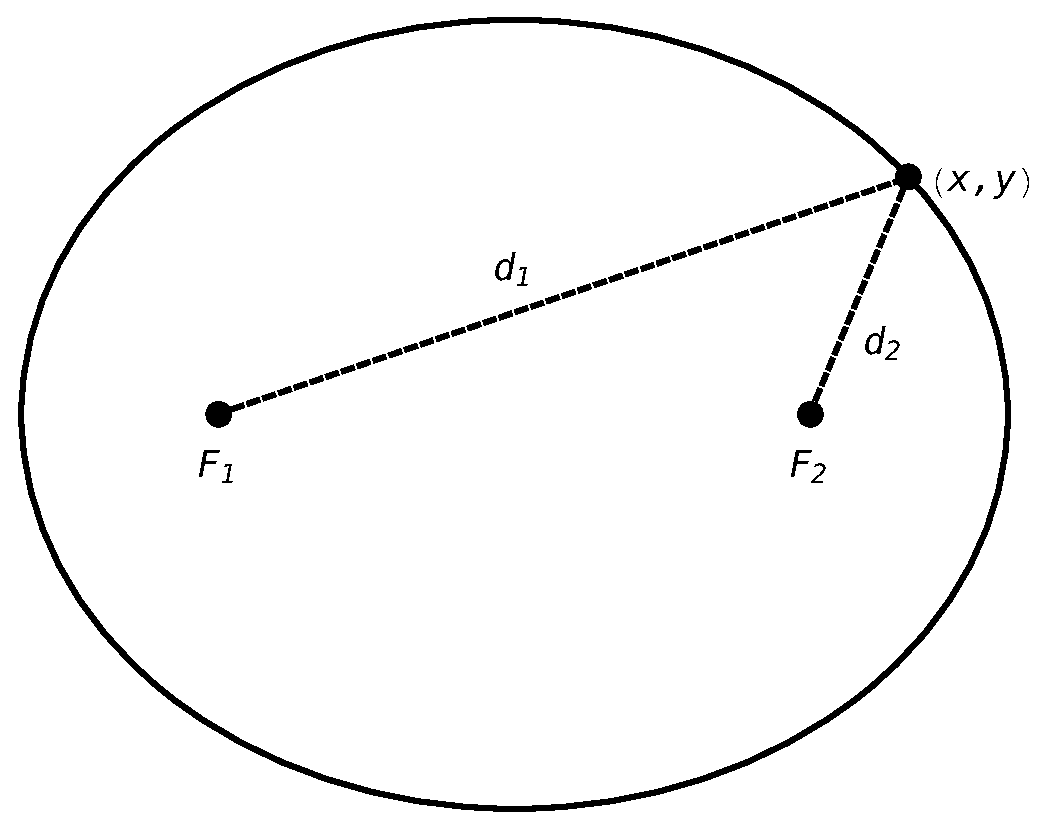
\includegraphics[width=0.4\textwidth]{fig_algebraic_21}
	\caption{$d_1 + d_2 = d$ for all $(x, y)$ on the ellipse.}
	\label{fig_algebraic_21}
	\end{center}
\end{figure}


The \index{ellipse ! centre} \index[aut]{ellips ! middelpunt} centre of the ellipse is the midpoint of the line connecting the two foci.  The \index{ellipse ! major axis}\index[aut]{ellips ! grote as}\textbf{major axis} (\textit{grote as}) of the ellipse is the line segment connecting two opposite ends of the ellipse which also contains the centre and foci.  The \index{ellipse ! minor axis}\index[aut]{ellips ! kleine as}\textbf{minor axis} (\textit{kleine as}) of the ellipse is the line segment connecting two opposite ends of the ellipse which contains the centre but is perpendicular to the major axis.  The \index{ellipse ! vertices} \index[aut]{ellipse ! top}  \textbf{vertices} (\textit{top}) of an ellipse are the points of the ellipse which lie on the major axis.  Notice that the centre is also the midpoint of the major axis (Figure~\ref{fig_algebraic_21}) and that the major axis is the longer of the two axes through the centre, and likewise, the minor axis is the shorter of the two. 

\begin{figure}
	\begin{center}
			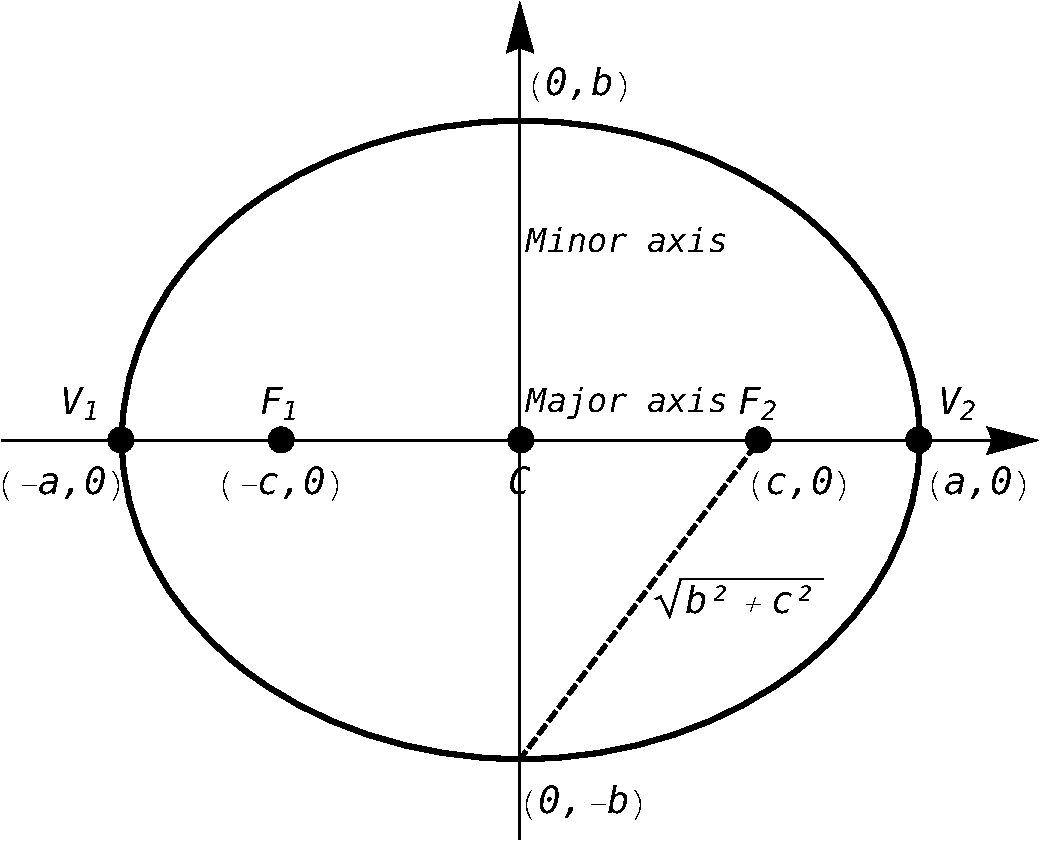
\includegraphics[width=0.5\textwidth]{fig_algebraic_22}
	\caption{An ellipse with centre $C$ $(0,0)$, foci $F_1$ $(-c,0)$, $F_2$ $(c,0)$ and vertices $V_1$ $(-a,0)$ and $V_2$ $(a,0)$.}
	\label{fig_algebraic_22}
	\end{center}
\end{figure}


\ifcourse
In order to derive the standard equation of an ellipse, we assume that the ellipse has its centre at $(0,0)$, its major axis along the $x$-axis, and has foci $(c,0)$ and $(-c,0)$ and vertices $(-a,0)$ and $(a,0)$ (Figure~\ref{fig_algebraic_22}).  We will label the $y$-intercepts of the ellipse as $(0,b)$ and $(0,-b)$. Moreover, we assume $a$, $b$, and $c$ are all positive numbers.

\ifanalysis
	\checkoddpage
\marginpar{\ifoddpage\hspace*{-1.5cm}\else\hspace*{0.25cm}\fi
\includegraphics[width=0.075\textwidth]{youtube}\\
\ifoddpage\hspace*{-1.75cm}\else\hspace*{0.1cm}\fi
\qrcode[height=1.75cm]{https://youtu.be/T5QTdGaCQes}
%\includegraphics[width=0.1\textwidth]{vergelijking_ellips}
}
 \fi
Note that since $(a,0)$ is on the ellipse, it must satisfy the conditions of Definition \ref{ellipsedefn}.  That is, the distance from $(-c,0)$ to $(a,0)$ plus the distance from  $(c,0)$ to $(a,0)$ must equal the fixed distance $d$.  Since all of these points lie on the $x$-axis, we get

\[ \begin{array}{rclr} 
 (a+c) + (a-c) & = & d & \\ \Leftrightarrow\quad 2a & = & d. \\ \end{array}\]


 We now use that fact $(0,b)$ is on the ellipse, along with the fact that $d=2a$ to get

\[ \begin{array}{rrcl} &\mbox{distance from  $(-c,0)$ to $(0,b)$} + \mbox{distance from $(c,0)$ to $(0,b)$} & = & 2a  \\ \Leftrightarrow&\sqrt{(0-(-c))^2+(b-0)^2} + \sqrt{(0-c)^2+(b-0)^2} & = & 2a   \\ 
\Leftrightarrow&2 \sqrt{b^2+c^2} & = & 2a \\ 
\Leftrightarrow&\sqrt{b^2+c^2} & = & a\,. \end{array}\]


From this, we get $a^2 = b^2 + c^2$, or $b^2 = a^2 - c^2$, which will prove useful later.  Now consider an arbitrary point $(x,y)$ on the ellipse.  Applying Definition~\ref{ellipsedefn}, we get


\[\allowdisplaybreaks \begin{array}{rrclr}  
&\sqrt{(x+c)^2+y^2}+\sqrt{(x-c)^2+y^2} & = & 2a  & \\ 
\Leftrightarrow&\sqrt{(x+c)^2+y^2} & = & 2a - \sqrt{(x-c)^2+y^2} & \\ 
%\left(\sqrt{(x+c)^2+y^2}\right)^2 & = & \left(2a - \sqrt{(x-c)^2+y^2}\right)^2 & \\ 
\Rightarrow&(x+c)^2+y^2 & = & 4a^2 - 4a\sqrt{(x-c)^2+y^2} + (x-c)^2+y^2 & \mbox{(Square both sides.)}\\ 
\Leftrightarrow&4a\sqrt{(x-c)^2+y^2} & = & 4a^2 + (x-c)^2 - (x+c)^2 & \\ 
\Leftrightarrow&4a\sqrt{(x-c)^2+y^2} & = & 4a^2 - 4cx & \\ 
\Leftrightarrow&a\sqrt{(x-c)^2+y^2} & = & a^2 - cx & \\ 
%\left(a\sqrt{(x-c)^2+y^2}\right)^2 & = & \left(a^2 - cx\right)^2 & \\ 
\Rightarrow&a^2\left((x-c)^2+y^2\right) & = & a^4 - 2a^2cx +c^2 x^2 & \mbox{(Square both sides.)}\\  
\Leftrightarrow&a^2x^2 - 2a^2cx + a^2c^2+a^2 y^2 & = & a^4 - 2a^2cx +c^2 x^2 & \\  
\Leftrightarrow&a^2x^2 - c^2 x^2 +a^2 y^2 & = & a^4  - a^2c^2 & \\ 
\Leftrightarrow&\left(a^2 - c^2\right) x^2 +a^2 y^2 & = & a^2 \left(a^2 - c^2\right)\,.  & \\ \end{array}\]

Recall now that $b^2 = a^2 - c^2$ so that

\[ \begin{array}{rrclr} 
&\left(a^2 - c^2\right)x^2 +a^2 y^2 & = & a^2\left(a^2 - c^2\right) & \\ 
\Leftrightarrow&b^2 x^2 +a^2 y^2 & = & a^2 b^2 & \\  
\Leftrightarrow&\dfrac{x^2}{a^2} + \dfrac{y^2}{b^2} & = & 1\,. &  \\ \end{array}\]

\medskip

This equation is for an ellipse centred at the origin. To get the formula for the ellipse centred at $(x_0,y_0)$, we could use the transformations from Section~\ref{sec_transformations} to obtain:
\begin{equation}
\dfrac{(x-x_0)^2}{a^2} + \dfrac{(y-y_0)^2}{b^2} = 1\,.
\label{standardellipse}
\end{equation}

\fi

\ifvc
We assume that the ellipse has its centre at $(0,0)$, its major axis along the $x$-axis, and has foci $(c,0)$ and $(-c,0)$ and vertices $(-a,0)$ and $(a,0)$ (Figure~\ref{fig_algebraic_22}).  We will label the $y$-intercepts of the ellipse as $(0,b)$ and $(0,-b)$. Moreover, we assume $a$, $b$, and $c$ are all positive numbers.
The standard equation for an ellipse centred at the origin is
\[ \dfrac{x^2}{a^2} + \dfrac{y^2}{b^2}  = 1\,.\]

\medskip

To get the formula for the ellipse centred at $(x_0,y_0)$, we could use the transformations from Section~\ref{sec_transformations} to obtain:
\begin{equation}
\dfrac{(x-x_0)^2}{a^2} + \dfrac{(y-y_0)^2}{b^2} = 1\,.
\label{standardellipse}
\end{equation}
\fi

Note that if $a > b$, then we have an ellipse whose major axis is horizontal, and hence, the foci lie to the left and right of the centre.   If $b > a$, the roles of the major and minor axes are reversed, and the foci lie above and below the centre.  Finally, it is worth mentioning that if $a=b$, we arrive at the standard equation of a circle. This indicates that it is fine to think of an ellipse as the deformation of a circle in which the circle is stretched farther in one direction than the other.


As with circles, an equation may be given which is an ellipse, but is not in the standard form of Equation~\eqref{standardellipse}.  In those cases,  we will need to massage the given equation into the standard form by taking the following steps:

\begin{enumerate}

\item  Group the same variables together on one side of the equation and position the constant on the other side.

\item  Complete the square in both variables as needed.

\item  Divide both sides by the constant term so that the constant on the other side of the equation becomes $1$.

\end{enumerate}



\begin{example} \label{ctsellipseex} 

Graph $x^2+4y^2-2x+24y+33 = 0$. Find the centre, the major and minor axes, the vertices, the endpoints of the minor axis, and the foci.


\xhrulefill{gray}{2.5pt}Solution \xhrulefill{gray}{2.5pt}


 Since we have a sum of squares and the squared terms have unequal coefficients, it is a good bet we have an ellipse on our hands.  We need to complete both squares, and then divide, if necessary, to get the right-hand side equal to $1$.
 \ifanalysis
 This ultimately leads to
 $$
 \dfrac{(x-1)^2}{4} + \dfrac{(y+3)^2}{1}  =  1\,.
 $$
\fi
\ifcalculus
\[ \begin{array}{rrclr} 
&x^2+4y^2-2x+24y+33 & = & 0 & \\
\Leftrightarrow&x^2-2x+4y^2+24y & = & -33 & \\
\Leftrightarrow&x^2 - 2x + 4\left(y^2+6y\right)  &  = & - 33 &  \\
\Leftrightarrow&\left(x^2 - 2x +1\right) + 4\left(y^2+6y+9\right)  &  = & - 33 + 1 + 4(9)& \\
\Leftrightarrow&(x-1)^2 + 4(y+3)^2  &  = & 4 & \\[5pt]  
\Leftrightarrow&\dfrac{(x-1)^2}{4} + \dfrac{(y+3)^2}{1} & = & 1& \\  \end{array} \]

\medskip
\fi

Now that this equation is in the standard form, we see that $x-x_0$ is $x-1$ so $x_0 = 1$, and $y-y_0$ is $y+3$ so $y_0 = -3$.  Hence, our ellipse is centred at $(1,-3)$.  We see that $a^2 = 4$ so $a=2$, and $b^2 = 1$ so $b=1$.  Consequently, the major axis will lie along the horizontal line $y=-3$, which means the minor axis lies along the vertical line $x = 1$. The vertices are the points on the ellipse which lie along the major axis so in this case, they are the points $(-1,-3)$ and $(3,-3)$, and the endpoints of the minor axis are $(1,-2)$ and $(1,-4)$. To find the foci, we find $c = \sqrt{4-1} = \sqrt{3}$, which means the foci lie $\sqrt{3}$ units from the centre. Since the major axis is horizontal, the foci lie $\sqrt{3}$ units to the left and right of the centre, at $(1-\sqrt{3},-3)$ and $(1+\sqrt{3},-3)$ (Figure~\ref{fig_algebraic_23}).  

\begin{figure}[H]
	\begin{center}
			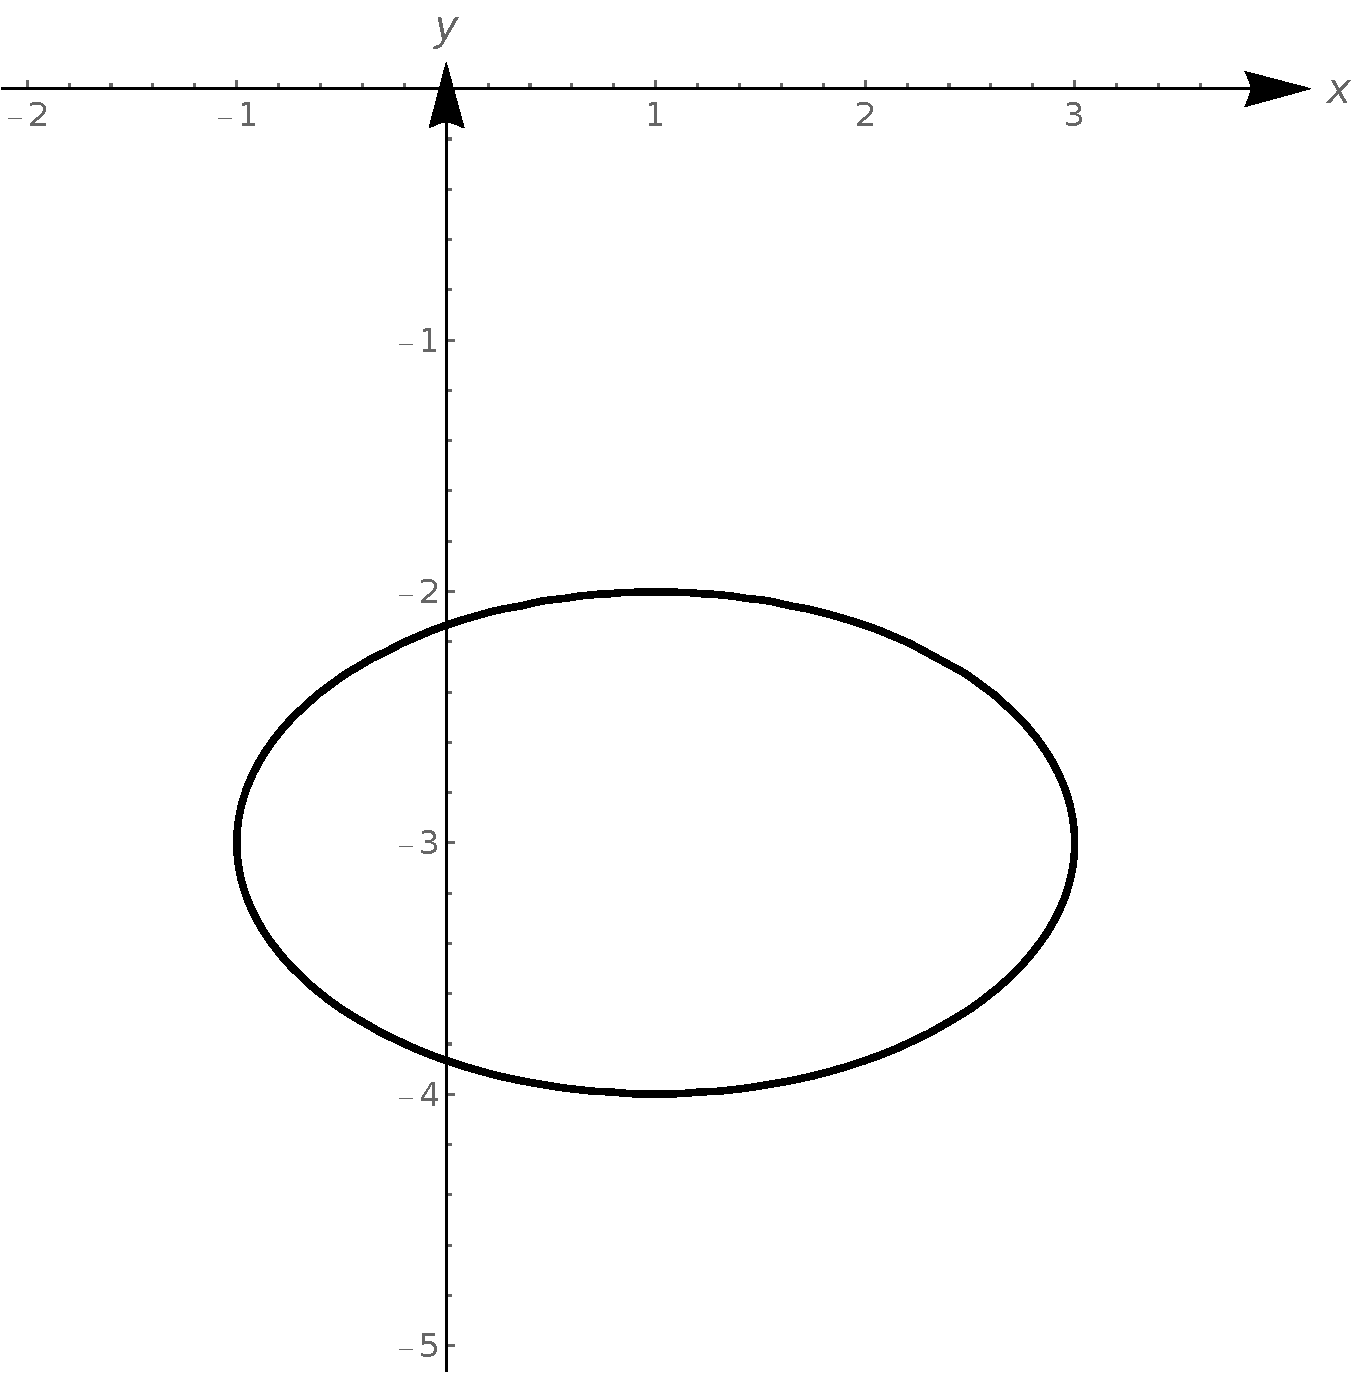
\includegraphics[width=0.5\textwidth]{fig_algebraic_23}
	\caption{Graph of $x^2+4y^2-2x+24y+33 = 0$.}
	\label{fig_algebraic_23}
	\end{center}
\end{figure}
\vspace*{-0.5cm}
\end{example}

\ifcourse
Johannes Kepler discovered that the orbits along which the planets travel around the Sun are ellipses with the Sun approximately at one focus (Figure~\ref{fig_algebraic_24}). A key feature of such planetary orbits are their eccentricity, which is a measure of the roundness of an ellipse and can be 
 quantified as below.

\begin{definition}[Eccentricity]

The \label{ellipseeccentricity} \index{ellipse ! eccentricity}\index{eccentricity}\index[aut]{ellipse ! excentriciteit}\index[aut]{excentriciteit} \textbf{eccentricity} (\textit{excentriciteit}) of an ellipse, denoted $e$, is the following ratio:

\[  e = \dfrac{\mbox{distance from the centre to a focus}}{\mbox{distance from the centre to a vertex}}. \]

\end{definition}

\begin{figure}
	\begin{center}
			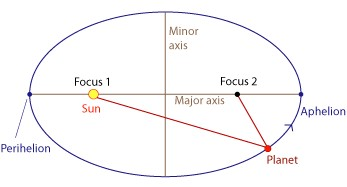
\includegraphics[width=0.5\textwidth]{fig_algebraic_24}
	\caption{An elliptical orbit of a planet.}
	\label{fig_algebraic_24}
	\end{center}
\end{figure}
From this definition, we infer that for a circle $e=0$, while we have for an ellipse that $e<1$.


Finally, it is important to underline that  ellipses have a  reflective property. If we imagine the dashed lines in Figure~\ref{fig_algebraic_21} representing sound waves, then the waves emanating from one focus reflect off the top of the ellipse and head towards the other focus.  Such geometry is exploited in the construction of so-called whispering galleries (Figure~\ref{fig_algebraic_25}). If a person whispers at one focus, a person standing at the other focus will hear the first person as if they were standing right next to them.  We explore this in our last example. 




\begin{example} \label{whisgalleryex}
Lisa and Jason want to exchange secrets from across a crowded whispering gallery. If the room is $40$ metres high at the centre and $100$ metres wide at the floor, how far from the outer wall should each of them stand so that they will be positioned at the foci of the ellipse? 

\xhrulefill{gray}{2.5pt}Solution \xhrulefill{gray}{2.5pt}

It is most convenient to imagine this ellipse centred at $(0,0)$.  Since the ellipse is $100$ units wide and $40$ units tall, we get $a=50$ and $b=40$.  Hence, our ellipse has the equation  
$$\frac{x^2}{50^2}+\frac{y^2}{40^2} = 1.$$
We are looking for the foci, and we get $c = \sqrt{50^2-40^2} = \sqrt{900} = 30$, so that the foci are $30$ units from the centre.  That means they are $50-30=20$ units from the vertices.  Hence, Jason and Lisa should stand $20$ metres from opposite ends of the gallery. 
\end{example}


\begin{figure}[h]
	\begin{center}
			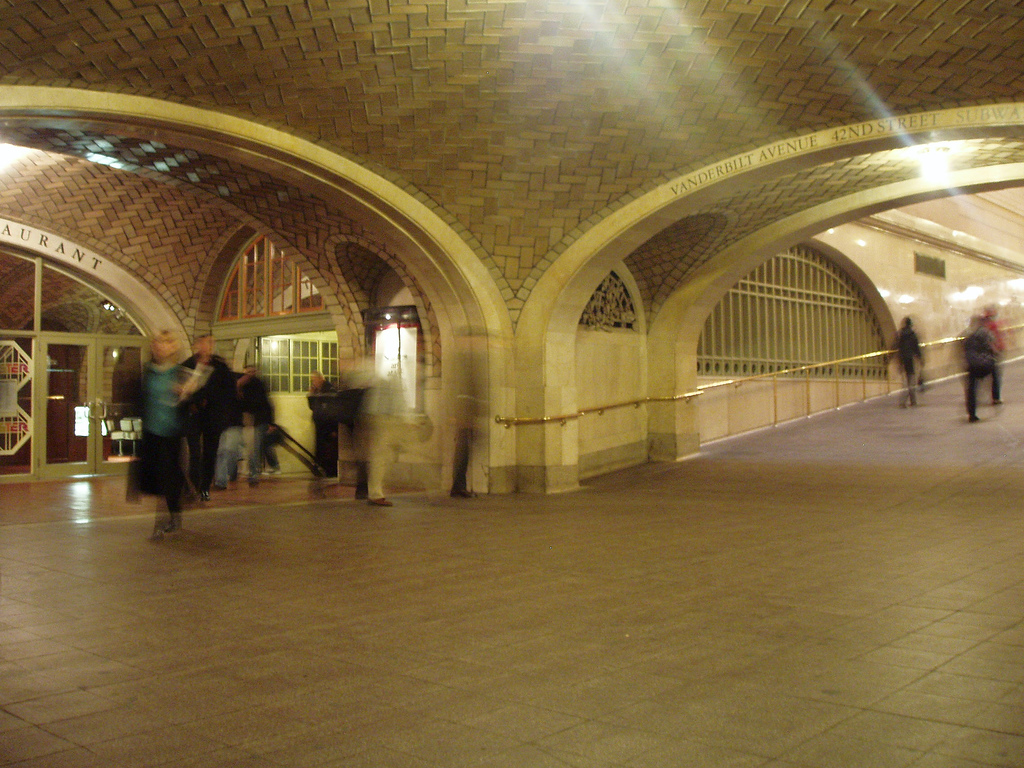
\includegraphics[width=0.4\textwidth]{fig_algebraic_25}
	\caption{Whispering gallery at Grand Central station, New York, United states.}
	\label{fig_algebraic_25}
	\end{center}
\end{figure}
\fi


\subsection{Parabolas}

We have already learned in Section~\ref{sec_pol} that the graph of a quadratic function $f(x) = ax^2 + bx + c$ ($a \neq 0$) is called a parabola.  We may also define parabolas in terms of distance.

\begin{definition}[Parabola]

\label{paraboladefn}

Let $F$ be a point in the plane and $d$ be a line not containing $F$. A \textbf{parabola} (\textit{parabool})\index{parabola}\index[aut]{parabool} is the set of all points equidistant from $F$ and $d$.  The point $F$ is called the \textbf{focus} (\textit{brandpunt})\index{parabola ! focus}\index[aut]{parabool ! brandpunt} of the parabola and the line $d$ is called the \textbf{directrix} (\textit{richtlijn})\index{parabola ! directrix}\index[aut]{parabool ! richtlijn} of the parabola.
\end{definition}

Essentially, in Figure~\ref{fig_algebraic_26}, each dashed line from the point $F$ to a point on the curve has the same length as the dashed line from the point on the curve to the line $d$.  The point $V$ is the \textbf{vertex} (\textit{top}).  The \index{parabola ! vertex}\index[aut]{parabool ! top}  vertex is the point on the parabola closest to the focus.



\begin{figure}
	\begin{center}
			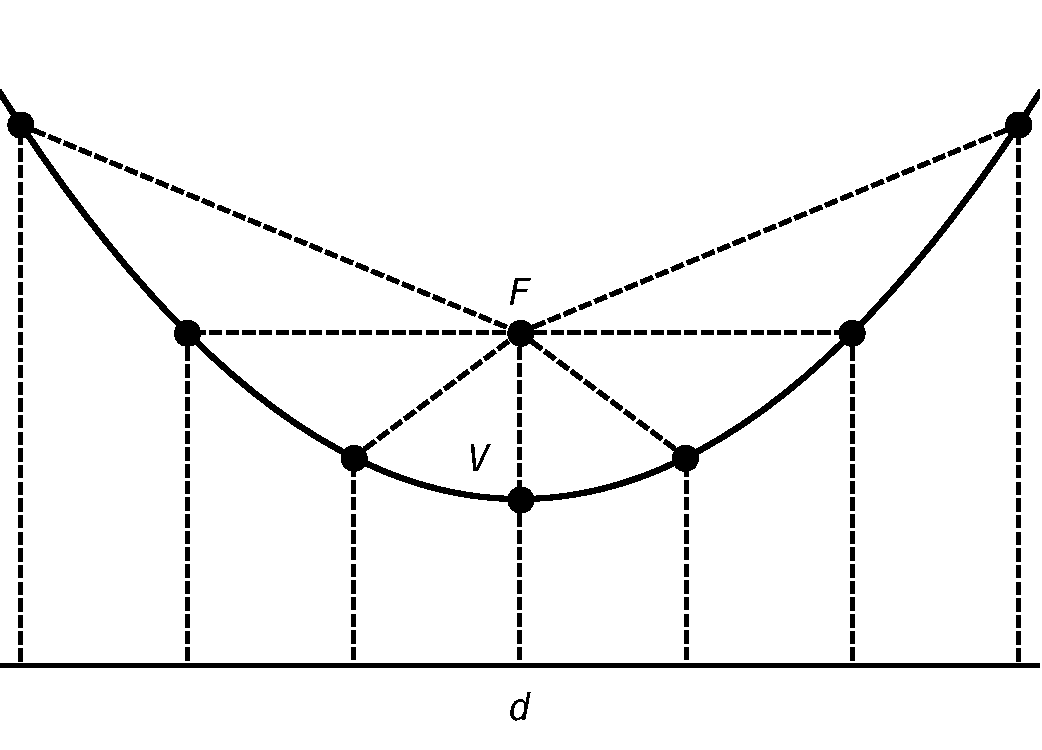
\includegraphics[width=0.5\textwidth]{fig_algebraic_26}
	\caption{Geometric construction a a parabola.}
	\label{fig_algebraic_26}
	\end{center}
\end{figure}

\ifcourse
We want to use only the distance definition of parabola to derive the equation of a parabola and we should get an expression much like those studied in Section \ref{sec_pol}.  Let $p$ denote the directed distance from the vertex to the focus, which by definition is the same as the distance from the vertex to the directrix.  For simplicity, assume that the vertex is $(0,0)$ and that the parabola opens upwards.  Hence, the focus is $(0,p)$ and the directrix is the line $y = -p$. All this is presented schematically in Figure~\ref{fig_algebraic_27}.
\fi

\ifvc
To get the standard equation of a parabola, let $p$ denote the directed distance from the vertex to the focus, which by definition is the same as the distance from the vertex to the directrix.  For simplicity, assume that the vertex is $(0,0)$ and that the parabola opens upwards.  Hence, the focus is $(0,p)$ and the directrix is the line $y = -p$. All this is presented schematically in Figure~\ref{fig_algebraic_27}.
\fi

\begin{figure}[h]
	\begin{center}
			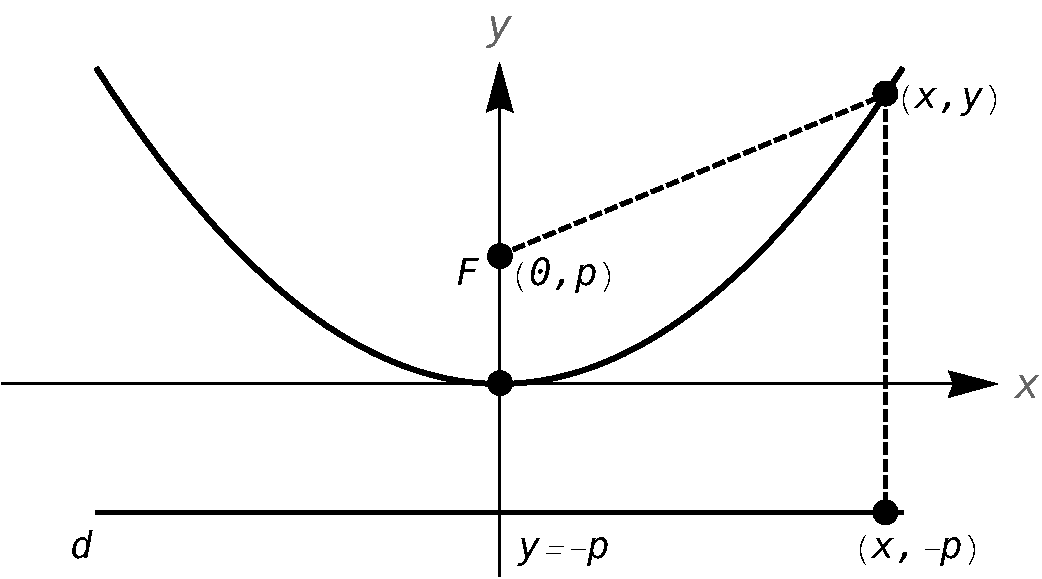
\includegraphics[width=0.5\textwidth]{fig_algebraic_27}
	\caption{Parabola with vertex in $(0,0)$, directrix $d: y=-p$ and focus $F (0,p)$.}
	\label{fig_algebraic_27}
	\end{center}
\end{figure}

\ifcourse
\ifanalysis
	\checkoddpage
\marginpar{\ifoddpage\hspace*{-1.5cm}\else\hspace*{0.25cm}\fi
\includegraphics[width=0.075\textwidth]{youtube}\\
\ifoddpage\hspace*{-1.75cm}\else\hspace*{0.1cm}\fi
\qrcode[height=1.75cm]{https://youtu.be/NDh57N7U2BU}
%\includegraphics[width=0.1\textwidth]{vergelijking_parabool}
}
 \fi
From the definition of parabola, we know that the distance from $(0,p)$ to $(x,y)$ is the same as the distance from $(x,-p)$ to $(x,y)$.  Using the distance formula, we get

\[ \begin{array}{rrclr} 
&\sqrt{(x -0)^2 + (y-p)^2} & = & \sqrt{(x-x)^2 + (y - (-p))^2} & \\
\Leftrightarrow&\sqrt{x^2 + (y-p)^2} & = & \sqrt{(y+p)^2} & \\
\Leftrightarrow&x^2 + (y-p)^2 & = & (y+p)^2 & \quad\mbox{(Square both sides.)} \\
\Leftrightarrow&x^2 + y^2 - 2py + p^2 & = & y^2 + 2py + p^2 & \quad\mbox{(Expand quantities.)} \\
\Leftrightarrow&x^2 & = & 4py. & \quad\mbox{(Gather like terms.)} \\ \end{array} \]
\fi

\ifvc
The standard equation is
\[ x^2  =  4py. \]
\fi

Solving for $y$ yields $y = \frac{x^2}{4p}$, which is a quadratic function of the form found in Definition~\ref{quadraticfunction} with $a = \frac{1}{4p}$ and vertex $(0, 0)$.


When $p < 0$, the parabola opens downwards.  In our formulation, we say that $p$ is a directed distance from the vertex to the focus:  if $p > 0$, the focus is above the vertex;  if $p < 0$, the focus is below the vertex.  If we choose to place the vertex at an arbitrary point $(x_0,y_0)$, we arrive at the standard equation of a vertical parabola  using the transformations from Section~\ref{sec_transformations}: 
\begin{equation}
 (x-x_0)^2 = 4p(y-y_0)\,.
\label{standardvparabola}
\end{equation}

Notice that in this standard equation, only one of the variables, $x$, is squared. This is a quick way to distinguish an equation of a parabola from that of a circle or ellipse because in the equation of a circle or ellipse, both variables are squared.

If we interchange the roles of $x$ and $y$, we can produce horizontal parabolas:  parabolas which open to the left or to the right.  The directrices of these would be vertical lines and the focus would either lie to the left or to the right of the vertex, as seen in Figure~\ref{fig_algebraic_28}. The standard equation of a horizontal parabola with vertex $(x_0,y_0)$  is
\begin{equation}
 (y-y_0)^2 = 4p(x-x_0)\,. 
\label{standardhparabola}
\end{equation}
If $p>0$, the parabola opens to the right;  if $p < 0$, it opens to the left.




As with circles and ellipses, not all parabolas will come to us in the forms in Equations \eqref{standardvparabola} or \eqref{standardhparabola}.  If we encounter an equation with two variables in which exactly one variable is squared, we can, however, put the equation into a standard form using the following steps.

\begin{enumerate}

\item  Group the variable which is squared on one side of the equation and position the non-squared variable and the constant on the other side.

\item  Complete the square if necessary and divide by the coefficient of the perfect square.

\item  Factor out the coefficient of the non-squared variable.

\end{enumerate}

\begin{figure}[h]
	\begin{center}
			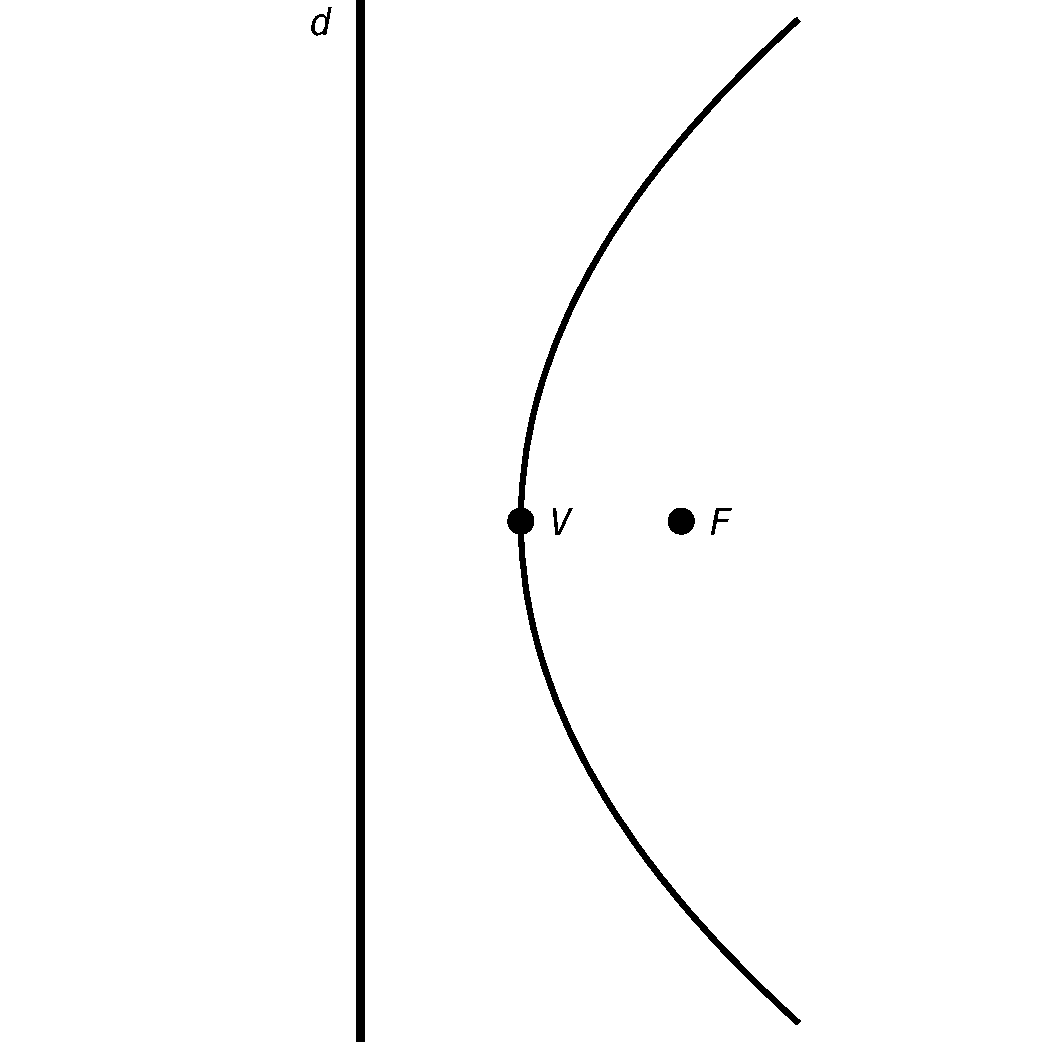
\includegraphics[width=0.4\textwidth]{fig_algebraic_28}
	\caption{Horizontal parabola opening to the right.}
	\label{fig_algebraic_28}
	\end{center}
\end{figure}

\begin{example} \label{ctsparabolaex} 
Consider the equation $y^2 + 4y + 8x = 4$.  Put this equation into standard form and graph the parabola.  Find the vertex, focus, and directrix.   

\xhrulefill{gray}{2.5pt}Solution \xhrulefill{gray}{2.5pt}

 We need a perfect square on the left-hand side of the equation and factor out the coefficient of the non-squared variable ($x$) on the other.
 \ifanalysis
 We finally arrive at:
 $$
 (y+2)^2  =  -8(x-1)\,.
 $$
 \fi

\ifcalculus
\[ \begin{array}{rrclr} 
&y^2+4y+8x &  = & 4 & \\
\Leftrightarrow&y^2 + 4y &  = & -8x + 4 &  \\
\Leftrightarrow&y^2+4y+4 & = & -8x+4+4 & \qquad\mbox{(Complete the square in $y$ only.)} \\
\Leftrightarrow&(y+2)^2 & = &-8x+8 & \qquad\mbox{(Factor.)}  \\ 
\Leftrightarrow&(y+2)^2 & = & -8(x-1) &   \end{array} \]
\fi

Now that the equation is in the form given in Equation \eqref{standardhparabola}, we see that  $x-x_0$ is $x-1$ so $x_0 = 1$, and  $y-y_0$ is $y+2$ so $y_0 = -2$.  Hence, the vertex is $(1,-2)$.  We also see that $4p = -8$ so that $p = -2$.  Since $p < 0$, the focus will be the left of the vertex and the parabola will open to the left.  The distance from the vertex to the focus is $|p| = 2$, which means the focus is $2$ units to the left of $1$, so if we start at $(1,-2)$ and move left $2$ units, we arrive at the focus $(-1,-2)$. The directrix, then, is $2$ units to the right of the vertex, so if we move right $2$ units from $(1,-2)$, we would be on the vertical line $x=3$.  Moreover, the parabola is $8$ units wide at the focus.

\begin{figure}[H]
	\begin{center}
			\includegraphics[width=0.4\textwidth]{fig_algebraic_29}
	\caption{Graph of $y^2+4y+8x=4$.}
	\label{fig_algebraic_29}
	\end{center}
\end{figure}

\end{example}

\ifcourse
Parabolas are used to model physical phenomena such as the trajectories of projectiles.  Other applications of the parabola concern its reflective property. If we imagine the dashed lines in Figure~\ref{fig_algebraic_30a} as emanating from the focus, we see that the waves are reflected off the parabola in a coherent fashion as in the case in a flash light.  Here, the bulb is placed at the focus and the light rays are reflected off a parabolic mirror to give directional light. This reasoning also works the other way around if we imagine the dashed lines below as electromagnetic waves heading towards a parabolic dish.  It turns out that the waves reflect off the parabola and concentrate at the focus which then becomes the optimal place for the receiver (Figure~\ref{fig_algebraic_30b}). 



\begin{figure}[H]
\centering
%\raisebox{0.5cm}{
\centerline{
\subfigure[\label{fig_algebraic_30a}]{\includegraphics[width=0.3\textwidth]{fig_algebraic_30a}}
\hspace{2cm}
\subfigure[ \label{fig_algebraic_30b}]{\includegraphics[width=0.2\textwidth]{fig_algebraic_30b}}
}

\caption{Reflective property of parabola (a) and a parabolic antenna making use thereof (b).}
\end{figure}



\begin{example} 
A satellite dish is to be constructed in the shape of a paraboloid of revolution.  If the receiver placed at the focus is located $2$ metres above the vertex of the dish, and the dish is to be $12$ metres wide, how deep will the dish be?

\xhrulefill{gray}{2.5pt}Solution \xhrulefill{gray}{2.5pt}

  One way to approach this problem is to determine the equation of the parabola suggested to us by this data.  For simplicity, we will assume the vertex is $(0,0)$ and the parabola opens upwards.  Our standard form for such a parabola is $x^2 = 4py$.  Since the focus is $2$ units above the vertex, we know  $p=2$, so we have $x^2 = 8y$.  Since the parabola is $12$ metres wide, we know the edge is $6$ metres from a vertical line through the vertex.  To find the depth, we are looking for the $y$ value when $x=6$.  Substituting $x=6$ into the equation of the parabola yields $6^2 = 8y$ or $y = 36/8 = 4.5$.  Hence, the dish will be  $4.5$ metres deep.  

\end{example}

Examples of parabolas occurring in nature are also manifold. For instance, rainbows and many natural bridges have a parabolic shape. Moreover, the trajectory traversed by jumping fish or aquatic mammals also approaches a parabola (Figure~\ref{fig_algebraic_31}). 


\begin{figure}[h]
\centering
%\raisebox{0.5cm}{
\centerline{
\subfigure[\label{fig_algebraic_31a}]{\includegraphics[width=0.33\textwidth]{fig_algebraic_31a}}
\hspace{0.1cm}
\subfigure[ \label{fig_algebraic_31b}]{\includegraphics[width=0.3\textwidth]{fig_algebraic_31b}}
\hspace{0.1cm}
\subfigure[\label{fig_algebraic_31c}]{\includegraphics[width=0.33\textwidth]{fig_algebraic_31c}}
}
\caption{Parabolas in nature: rainbow (a), natural bridge (b) and trajectories of jumping dolphins. \label{fig_algebraic_31}}
\end{figure}
\fi



\subsection{Hyperbolas}
In the definition of an ellipse, Definition \ref{ellipsedefn}, we fixed two points called foci and looked at points whose distances to the foci always added to a constant distance $d$.  But what, if any, curve we would generate if we replaced added with subtracted.  The answer is a hyperbola.

\begin{definition}[Hyperbola] \label{hyperboladefn} 
Given two distinct points $F_1$ and $F_2$ in the plane and a fixed distance $d$, a \textbf{hyperbola} (\textit{hyperbool})
\index{hyperbola}\index[aut]{hyperbool} is the set of all points $(x, y)$ in the plane such that the absolute value of the difference of each of the distances from $F_1$ and $F_2$  to $(x, y)$ is $d$. The points $F_1$ and $F_2$ are called the \textbf{foci} (\textit{brandpunten}) \index{hyperbola ! foci}\index[aut]{hyperbool ! brandpunten} of the hyperbola.

\end{definition} 


Note that the hyperbola has two parts, called \index{hyperbola ! branch}\index[aut]{hyperbool ! tak} \textbf{branches} (\textit{tak}).  The \index{hyperbola ! centre}\index[aut]{hyperbool ! middelpunt}\textbf{centre} (\textit{middelpunt}) of the hyperbola is the midpoint of the line connecting the two foci.  The \index{hyperbola ! transverse axis}\index[aut]{hyperbool ! hoofdas}\textbf{transverse axis} (\textit{hoofdas}) of the hyperbola is the line segment connecting two opposite ends of the hyperbola which also contains the centre and foci.  The \index{hyperbola ! vertices}\index[aut]{hyperbool ! top}\textbf{vertices} (\textit{top}) of a hyperbola are the points of the hyperbola which lie on the transverse axis.  In addition, there are lines called \index{hyperbola ! asymptotes}\index[aut]{hyperbool ! asymptoot}\textbf{asymptotes} (\textit{asymptoot}) which the branches of the hyperbola approach for large $x$- and $y$-values (Figure~\ref{fig_algebraic_32}).  The \index{hyperbola ! conjugate axis}\index[aut]{hyperbool ! nevenas}\textbf{conjugate axis} (\textit{nevenas}) of a hyperbola is the line through the centre which is perpendicular to the transverse axis. It contains two \textbf{imaginary vertices} (\textit{imaginaire toppen}).
\index{hyperbola! imaginary vertices}\index[aut]{hyperbool ! imaginaire toppen}

\begin{figure}[H]
	\begin{center}
			\includegraphics[width=0.4\textwidth]{fig_algebraic_32}
	\caption{A hyperbola with centre $C$; foci $F_1$, $F_2$; and vertices $V_1$, $V_2$ and asymptotes (dashed)}
	\label{fig_algebraic_32}
	\end{center}
\end{figure}

\ifcourse
Suppose now we wish to derive the equation of a hyperbola.  For simplicity, we shall assume that the centre is $(0,0)$,  the vertices are $(a,0)$ and $(-a,0)$ and the foci are $(c,0)$ and $(-c,0)$.  We label the endpoints of the conjugate axis $(0,b)$ and $(0,-b)$. Although $b$ does not enter into our derivation, we will have to justify this choice as you shall see later. As before, we assume $a$, $b$, and $c$ are all positive numbers.  Schematically we get the picture shown in Figure~\ref{fig_algebraic_33}. 
\fi

\ifvc
To get the equation of a hyperbola centred at the origin, we shall assume that the centre is $(0,0)$,  the vertices are $(a,0)$ and $(-a,0)$ and the foci are $(c,0)$ and $(-c,0)$.  We label the endpoints of the conjugate axis $(0,b)$ and $(0,-b)$.  (Although $b$ does not enter into our derivation, we will have to justify this choice as you shall see later.)  As before, we assume $a$, $b$, and $c$ are all positive numbers.  Schematically we get the picture shown in Figure~\ref{fig_algebraic_33}. 
\fi

\begin{figure}[h]
	\begin{center}
			\includegraphics[width=0.5\textwidth]{fig_algebraic_33}
	\caption{A hyperbola with centre in $(0,0)$; foci $F_1 (-c,0)$, $F_2 (c,0)$; and vertices $V_1 (-a,0)$, $V_2 (a,0)$, imaginary vertices $(0,-b)$ and $(0,b)$, and asymptotes (dashed).}
	\label{fig_algebraic_33}
	\end{center}
\end{figure}


\ifcourse
Since $(a,0)$ is on the hyperbola, it must satisfy the conditions of Definition~\ref{hyperboladefn}.  That is, the distance from $(-c,0)$ to $(a,0)$ minus the distance from $(c,0)$ to $(a,0)$ must equal the fixed distance $d$.  Since all these points lie on the $x$-axis, we get

\[ \begin{array}{rrcl} &\mbox{distance from $(-c,0)$ to $(a,0)$} - \mbox{distance from $(c,0)$ to $(a,0)$} & = & d  \\
\Leftrightarrow&(a+c) - (c-a) & = & d  \\
\Leftrightarrow&2a & = & d. \\ \end{array}\]

\medskip

Hence, $d$ is the distance between the vertices $V_1$ and $V_2$.

Now consider a point $(x,y)$ on the hyperbola.  Applying Definition~\ref{hyperboladefn}, we get


\[ \begin{array}{rrclr} 
&\left|\mbox{distance from  $(-c,0)$ to $(x,y)$} - \mbox{distance from $(c,0)$ to $(x,y)$} \right|& = & 2a & \\ 
\Leftrightarrow&\left|\sqrt{(x-(-c))^2+(y-0)^2} - \sqrt{(x-c)^2+(y-0)^2} \right|& = & 2a & \\ 
\Leftrightarrow&\left|\sqrt{(x+c)^2+y^2} - \sqrt{(x-c)^2+y^2} \right|& = & 2a \,. \\ \end{array}\]

\medskip

Following the same procedure as when deriving the standard formula of an ellipse (Equation~\eqref{standardellipse}), we arrive at:

\[ \begin{array}{rclr} \left(a^2 - c^2\right) x^2 +a^2 y^2 & = & a^2 \left(a^2 - c^2\right)\,.  & \end{array}\]

What remains is to determine the relationship between $a$, $b$ and $c$.  To that end, we note that since $a$ and $c$ are both positive numbers with $a < c$, we get $a^2 < c^2$ so that $a^2 - c^2$ is a negative number.  Hence, $c^2 - a^2$ is a positive number. Let us rewrite the equation by solving for $y^2/x^2$ to get
 
\[ \begin{array}{rrclr} 
&\left(a^2 - c^2\right) x^2 +a^2 y^2 & = & a^2 \left(a^2 - c^2\right)  & \\
\Leftrightarrow&-\left(c^2 - a^2\right) x^2 +a^2 y^2 & = & -a^2 \left(c^2 - a^2\right)  & \\
\Leftrightarrow&a^2 y^2 & = &  \left(c^2 - a^2\right) x^2 -  a^2\left(c^2 - a^2\right)& \\
\Leftrightarrow&\dfrac{y^2}{x^2} & = &  \dfrac{\left(c^2 - a^2\right)}{a^2} -  \dfrac{\left(c^2 - a^2\right)}{x^2}\,.& \\ \end{array}\]

As $x$ and $y$ attain very large values, the quantity $\frac{\left(c^2 - a^2\right)}{x^2} \rightarrow 0$ so that $\frac{y^2}{x^2}  \rightarrow  \frac{\left(c^2 - a^2\right)}{a^2}$.  By setting \\ $b^{2} = c^{2} - a^{2}$ we get 
$\frac{y^2}{x^2}  \rightarrow  \frac{b^2}{a^2}$.  This shows that $y \rightarrow \pm \frac{b}{a} x$ as $|x|$ grows large.  Thus $y = \pm \frac{b}{a} x$ are the asymptotes to the graph. In our equation of the hyperbola we can substitute $a^2 - c^2 = -b^2$ which yields 

\[ \begin{array}{rrclr} 
&\left(a^2 - c^2\right) x^2 +a^2 y^2 & = & a^2 \left(a^2 - c^2\right)  &\\
\Leftrightarrow&-b^2 x^2 +a^2 y^2 & = & - a^2 b^2  & \\
\Leftrightarrow&\dfrac{x^2}{a^2} - \dfrac{y^2}{b^2} & = & 1\,. & \end{array} \]

The equation above is for a hyperbola whose centre is the origin and which opens to the left and right.  
\fi

\ifvc
The standard equation for an hyperbola whose centre is the origin and which opens to the left and right:
\[\dfrac{x^2}{a^2} - \dfrac{y^2}{b^2} =  1\,. \]  
\fi


If the hyperbola were centred at a point $(x_0, y_0)$, we would get the following: 
\begin{equation}
\dfrac{(x-x_0)^2}{a^2} - \dfrac{(y-y_0)^2}{b^2} = 1\,.
\label{standardhhyperbola}
\end{equation}

If the roles of $x$ and $y$ were interchanged, then the hyperbola's branches would open upwards and downwards and we would get a vertical hyperbola. Its standard equation is given by
\begin{equation}
\dfrac{(y-y_0)^2}{b^2} - \dfrac{(x-x_0)^2}{a^2} = 1\,.
\label{standardvhyperbola}
\end{equation}
By convention, $a$ always refers to the coefficient in the denominator of the term containing $x^2$, while $b$ refers to the coefficient appearing in the denominator of the term containing $y^2$. 

The distance from the centre to the foci, $c$, as seen in the derivation, can be found by the formula $c = \sqrt{a^2 + b^2}$.  Also note that we can quickly distinguish the equation of a hyperbola from that of a circle or ellipse because the hyperbola formula involves a difference of squares where the circle and ellipse formulas both involve the sum of squares.

 \ifvc 
As with the other conic sections, an equation whose graph is a hyperbola may not be given in either of the standard forms. To rectify that, we may follow the following steps.


 \begin{enumerate}

\item  Group the same variables together on one side of the equation and position the constant on the other side.

\item  Complete the square in both variables as needed.

\item  Divide both sides by the constant term so that the constant on the other side of the equation becomes $1$.

\end{enumerate}
\fi

\ifvc
\begin{example}
 \label{ctshyperbolaex} 
Consider the equation $9y^2-x^2-6x=10$.  Put this equation in to standard form and graph.  Find the center, the transverse and conjugate axes, the vertices, the foci, and the equations of the asymptotes.   

\xhrulefill{gray}{2.5pt}Solution \xhrulefill{gray}{2.5pt}


We need only complete the square on $x$ and rewrite the resulting equation in standard form:

\[ \begin{array}{rrclr} 
&9y^2-x^2-6x & = & 10 & \\[5pt]
\Leftrightarrow&9y^2-\left(x^2+6x\right) &  = & 10 &  \\[5pt]
\Leftrightarrow&9y^2-\left(x^2+6x + 9\right) &  = & 10 - 9 &  \\[5pt]
\Leftrightarrow&9y^2-(x+3)^2 &  = & 1 &  \\ [5pt]
\Leftrightarrow&\dfrac{y^2}{\frac{1}{9}} - \dfrac{(x+3)^2}{1} & = & 1\,.&  \end{array} \]


Now that this equation is in the standard form of Equation \ref{standardvhyperbola}, we see that $x-x_0$ is $x+3$ so $x_0 = -3$, and $y-y_0$ is $y$ so $y_0 = 0$.  Hence, our hyperbola is centred at $(-3, 0)$.  We find that $a^2 = 1$ so $a=1$, and $b^2 = 1/9$ so  $b=1/3$.  

Since the $x^2$ term is being subtracted from the $y^2$ term, we know the branches of the hyperbola open upwards and downwards.  This means the transverse axis lies along the vertical line $x=-3$ and the conjugate axis lies along the $x$-axis.  Since the vertices of the hyperbola are where the hyperbola intersects the transverse axis, we get that the vertices are $1/3$ of a unit above and below $(-3, 0)$ at $\left(-3, 1/3\right)$ and $\left(-3, -1/3\right)$.  To find the foci, we use 
$$
c = \sqrt{a^2 + b^2} = \sqrt{\frac{1}{9} + 1} = \frac{\sqrt{10}}{3}\,.
$$
Since the foci lie on the transverse axis, we arrive at $\left(-3, \sqrt{10}/3\right)$ and $\left(-3, -\sqrt{10}/3\right)$.  To determine the asymptotes, recall that the asymptotes have slopes of $\pm \frac{b}{a} = \pm \frac{1}{3}$.  So we get  $y = \frac{1}{3}x + 1$ and $y = -\frac{1}{3}x - 1$.  Putting it all together, we get the hyperbola shown in Figure~\ref{fig_algebraic_34}.


\begin{figure}[H]
	\begin{center}
			\includegraphics[width=0.4\textwidth]{fig_algebraic_34}
	\caption{Graph of $9y^2-x^2-6x=10$.}
	\label{fig_algebraic_34}
	\end{center}
\end{figure}


\end{example}
\fi

\ifcourse
Determining the location of a known event has many practical uses such as: locating the epicentre of an earthquake, an airplane crash site, the position of the person speaking in a large room, etc..  To determine the location of an earthquake's epicentre, seismologists use trilateration. A seismograph allows one to determine how far away the epicentre was; using three separate readings, the location of the epicentre can be approximated.


\begin{example}
Consider three microphones at positions $A$, $B$ and $C$ which all record a noise (a person's voice, an explosion, etc.) created at unknown location $D$. The microphone does not know when the sound was created, only when the sound was detected. How can the location be determined in such a situation?

\xhrulefill{gray}{2.5pt}Solution \xhrulefill{gray}{2.5pt}

If each location has a clock set to the same time, hyperbolas can be used to determine the location. Suppose the microphone at position $A$ records the sound at exactly 12:00, location $B$ records the time exactly 1 second later, and location $C$ records the noise exactly 2 seconds after that. We are interested in the difference of times. Since the speed of sound is approximately 340 m/s, we can conclude quickly that the sound was created 340 meters closer to position $A$ than position $B$. If $A$ and $B$ are a known distance apart (as shown in Figure \ref{fig_algebraic_35a}), then we can determine a hyperbola on which $D$ must lie. 

The difference of distances between $A$ and $B$ is $340$ metres; this is also the distance between vertices of the hyperbola. So we know $2a= 340$. Positions $A$ and $B$ lie on the foci, so $2c=1000$. From this we can find $b\approx 470$ and can sketch the hyperbola, with equation 
$$
\dfrac{x^2}{170^2}-\dfrac{y^2}{470^2}=1\,,
$$
whose graph is shown in Figure \ref{fig_algebraic_35b}. We only care about the side closest to $A$ because the sound was first heard at that location.

We can also find the hyperbola defined by positions $B$ and $C$. In this case, $2b = 680$ as the sound travelled an extra 2 seconds to get to $C$. We still have $2c=1000$, centring this hyperbola at $(-500,500)$. We find $a\approx 367$. This hyperbola has equation 
$$
\dfrac{(y-500)^2}{340^2}-\dfrac{(x+500)^2}{367^2}=1\,,
$$
and is sketched in Figure~\ref{fig_algebraic_35c}. The intersection point of the two graphs is the location of the sound, at approximately $(188,-222.5)$.


\begin{figure}[H]
\centering
%\raisebox{0.5cm}{
\centerline{
\subfigure[\label{fig_algebraic_35a}]{\includegraphics[width=0.33\textwidth]{fig_algebraic_35a}}
\hspace{0.1cm}
\subfigure[ \label{fig_algebraic_35b}]{\includegraphics[width=0.33\textwidth]{fig_algebraic_35b}}
\hspace{0.1cm}
\subfigure[\label{fig_algebraic_35c}]{\includegraphics[width=0.33\textwidth]{fig_algebraic_35c}}
}
\caption{An example of trilateration using hyperbolas. }
\end{figure}

\end{example}



	\begin{center}
 \vspace{2cm}
			\includegraphics[width=0.75\textwidth]{GreatMath_2.jpg}
	\end{center}
\fi


%%%%%%%%%%%%%%%%%%%%%%%%%%
%Oefeningen cursus
%%%%%%%%%%%%%%%%%%%%%%%%%%
\ifcourse %Begin oefeningen in de cursus 
\newpage
\section{Exercises}

\renewcommand{\ExerciseListName}{Opgave}

\subsection*{\nameref{sec_pol}}


%%%%%%%%%%%%%%%%%
%Oefening 1
%%%%%%%%%%%%%%%%%
\begin{Exercise} Draw and describe the following areas. 
	\begin{multicols}{2}
        \Question[difficulty = 1] $y \leq x-1$ 
        \ifanalysis\Question[difficulty = 1]\fi\ifcalculus\Question[difficulty = 2]\fi $|x|-4 < y < 2-x$ 
        \Question[difficulty = 1] $x^2 \leq y < x+2$
	    \Question[difficulty = 1] $x^2+2x+y^2 <8$ 
	    \ifanalysis\Question[difficulty = 1]\fi\ifcalculus\Question[difficulty = 2]\fi $x^2+y^2 < 2x, \quad x^2+y^2 < 2y$ 
	    \Question[difficulty = 2] $x^2+y^2-4x+2y >4, \quad x+y>1$  
	    \EndCurrentQuestion
    \end{multicols}

\end{Exercise}
\setboolean{firstanswerofthechapter}{true}
\begin{Answer}\phantom{}
    
	\Question All points located in the half plane under the line $y=x-1$, including the points on the line. 
	\Question All points located in the area between the lines $y=-x-4$, $y=x-4$ and $y=2-x$, which includes the origin. 
	\Question All points located in the region understood between the line $y=x+2$ and the parabola $y=x^2$, including points on the parabola. 
	\Question All points located within the circle with center $(-1,0)$ and radius 3.
	\Question All points located within the circle with center $(1,0)$ and radius 1 \' and within the circle with center $(0,1)$ and radius 1.
	\Question All points located outside the circle with center $(2,-1)$ and radius 3 \' and to the right of the line $x+y=1$.

\end{Answer}
\setboolean{firstanswerofthechapter}{false}


	


%%%%%%%%%%%%%%%%%
%Oefening 5
%%%%%%%%%%%%%%%%%
\begin{Exercise} Factorize the polynomials below into real factors. 
    \begin{multicols}{2}
        \ifanalysis\Question[difficulty = 1]\fi\ifcalculus\Question[difficulty = 2]\fi $2x^6-128$ 
        \Question[difficulty = 1] $8x^3+12x^2+6x+1$ 
        \ifanalysis\Question[difficulty = 1]\fi\ifcalculus\Question[difficulty = 2]\fi $2x^3+3x^2+2x+3$ 
        \Question[difficulty = 1] $x^4-7x^3+18x^2-20x+8$ 
        \Question[difficulty = 1] $x^4+x^3-2x^2-4x-8$
        \Question[difficulty = 1] $2x^3-3x^2-3x+2$
    	\ifanalysis\Question[difficulty = 1]\fi\ifcalculus\Question[difficulty = 2]\fi $8a^3-60a^2b+150ab^2-125b^3$
    	\Question[difficulty = 2] $a^2-2a+1-b^2-4bc-4c^2$
    	%\item $125x^3-8y^3+12y^2z-6yz^2+z^3$
    	\Question[difficulty = 3] $x^3-4x^2y+7xy^2-4y^3$
    	\Question[difficulty = 3] $2(x^2+6x+1)^2+5(x^2+6x+1)(x^2+1)+2(x^2+1)^2$
    	\EndCurrentQuestion
    \end{multicols}

\end{Exercise}

\begin{Answer}\phantom{}
    \begin{multicols}{2}
	
        \Question $2(x-2)\left(x^2+2x+4 \right)(x+2)\left(x^2-2x+4 \right)$ %OK
        \Question $(2x+1)^3$ %OK
        \Question $\left(x^2+1\right)\left(2x+3\right)$ %OK
        \Question $(x-2)^3(x-1)$ %OK
        \Question $(x-2)(x+2) \left(x^2+x+2 \right)$ %OK
        \Question $(2x-1)(x+1)(x-2)$ %OK
        \Question $(2a-5b)^3$ %OK
        \Question $(a-1-b-2c)(a-1+b+2c)$ %OK
        \Question $(x-y)(x^2-3xy+4y^2)$ %OK
        \Question $9(x+1)^2(x^2+4x+1)$ %OK
        %\Question $(x+2)\left(x^4-2x^3+4x^2-8x+16 \right) + 8 $ 
        %\Question $(a+1) \left(4a^3-4a^2+4a-7 \right)$ 
	\EndCurrentQuestion
	\end{multicols}
\end{Answer}

%%%%%%%%%%%%%%%%%
%Oefening 6
%%%%%%%%%%%%%%%%%
\begin{Exercise} Write each polynomial as a product of real factors. 
	 \begin{multicols}{2}
 		\Question[difficulty = 1] $16x^4-8x^2+1$
 		\Question[difficulty = 1] $x^4-1$
 		\Question[difficulty = 1] $x^5-x^4-16x+16$
 		\Question[difficulty = 2] $x^5+x^3+8x^2+8$
 		\Question[difficulty = 1] $x^4+6x^3+9x^2$
 		\ifanalysis\Question[difficulty = 1]\fi\ifcalculus\Question[difficulty = 2]\fi $x^6-3x^4+3x^2-1$
 		\ifanalysis\Question[difficulty = 1]\fi\ifcalculus\Question[difficulty = 2]\fi $x^9-4x^7-x^6+4x^4$
 		\EndCurrentQuestion
    \end{multicols}

\end{Exercise}

\begin{Answer}\phantom{}
    
	\Question $16x^4 - 8x^2 + 1 = (2x + 1)^2(2x - 1)^2 = (4x^2 - 1)^2$
	\Question $x^4 - 1 = (x^2 + 1)(x + 1)(x - 1)$
	\Question $x^5 - x^4 - 16x + 16 = (x - 2)(x + 2)(x^2 + 4)(x - 1)$
	\Question $x^5 + x^3 + 8x^2 + 8 = (x^2+1)(x+2)(x^2-2x+4)$
	\Question $x^4+6x^3+9x^2 = x^2 (x+3)^2$
	\Question $x^6-3x^4+3x^2-1 = (x-1)^3(x+1)^3$
	\Question $x^9-4x^7-x^6+4x^4 = x^4 (x-2) (x-1) (x+2) (x^2+x+1)$
\end{Answer}
 
%\pagebreak
%%%%%%%%%%%%%%%%%
%Oefening 7
%%%%%%%%%%%%%%%%%
\begin{Exercise} Solve the equations below in $\mathbb{C}$ and determine both the real and complex decomposition.
 	\begin{multicols}{2}
     	\Question[difficulty = 1] $ x^3-3x^2+20=0$	
     	\Question[difficulty = 1] $ 2x^3-4x^2-10x+12=0$	
     	\ifanalysis\Question[difficulty = 1]\fi\ifcalculus\Question[difficulty = 2]\fi $ x^6-16x^3+64=0$	
     	\ifanalysis\Question[difficulty = 1]\fi\ifcalculus\Question[difficulty = 2]\fi $8x^4-20x^3+18x^2-7x+1=0$ 	
     	\Question[difficulty = 1] $ x^3-16x^2+48x+72=0$
     	\Question[difficulty = 1] $4x^3-14x^2+8x+8 =0$
     	\Question[difficulty = 1] $x^5 + 6x^4 + x^3 - 26 x^2 - 32=0 $ 
     	\Question[difficulty = 1] $-2x^6-10x^5-16x^4-8x^3 =0$
     	\EndCurrentQuestion
 	\end{multicols}
 
\end{Exercise}

\begin{Answer}\phantom{}
    
    \Question $ x^3-3x^2+20 = (x+2)(x^2-5x+10) = (x+2) \left( x- \dfrac{5+\sqrt{15}i}{2}\right) \left( x- \dfrac{5-\sqrt{15}i}{2}\right)$ \\
    real zeros: $x=-2$, complex zeros: $x=\dfrac{5 \pm \sqrt{15}i}{2}$
 	\Question $ 2x^3-4x^2-10x+12 = 2(x-3)(x-1)(x+2)$ \\
 	real zeros: $x=3$, $x=1$ and $x=-2$
 	\Question $x^6-16x^3+64 = (x^3-8)^2 = (x-2)^2(x^2+2x+4)^2 =(x-2)^2 \left(x+1 -\sqrt{3}i\right)^2\left(x+1 +\sqrt{3}i\right)^2$\\
 	real zeros: $x=2$ (2x),  complex zeros: $x=-1 \pm \sqrt{3}i$ (2x)
 	\Question $8x^4-20x^3+18x^2-7x+1 = (x-1)(2x-1)^3$\\
 	real zeros: $x = \dfrac{1}{2}$ (3x) and $x = 1$
 	\Question $x^3-16x^2+48x+72=(x-6)\left(x-5-\sqrt{37} \right)\left(x-5+\sqrt{37} \right)$	\\ 
 	real zeros: $x=6$, $x=5+\sqrt{37}$ and $x=5-\sqrt{37}$
 	\Question $4x^3-14x^2+8x+8 = 4(x-2)^2 \left(x+\dfrac{1}{2}\right)$ \\ 
 	real zeros: $x=2$ (2x) and $x=-\dfrac{1}{2}$
 	\Question $x^5 + 6x^4 + x^3 - 26 x^2 - 32= (x^3 + 6x^2 - 32)(x^2+1) = (x-2)(x+4)^2 (x-i)(x+i)$ \\ 
 	real zeros: $x=2$ and $x=-4$ (2x), complex zeros: $x=\pm i$
 	\Question $-2x^6-10x^5-16x^4-8x^3=-2x^3(x+1)(x+2)^2$ \\ 
 	real zeros: $x=0$ (3x), $x=-1$ and $x=-2$ (2x)
\end{Answer}
 	
%%%%%%%%%%%%%%%%%
%Oefening 8 Bio-irs
%%%%%%%%%%%%%%%%%

\ifanalysis
\begin{Exercise}[difficulty = 2] Determine $a$ and $b$ such that
    	\Question $2x^3+ax^2+bx-3$ has $-1$ and $3$ as zeros.
    	\Question $ax^3+19x^2+bx+8$ is divisible by $x+2$ and $x+4$.

\end{Exercise}

\begin{Answer}\phantom{}
    
    \Question $a=-3, b=-8$
    \Question $a=3, b= 30 $
\end{Answer}

\fi

%%%%%%%%%%%%%%%%%
%Oefening 9 Bio-irs
%Oefening 8 Ings
%%%%%%%%%%%%%%%%%
\begin{Exercise} Solve the equation below in $\mathbb{R}$. Write the set of solutions as an interval.
	\begin{multicols}{2}
    	\Question[difficulty = 1] $-2x^3+19x^2-49x+20>0 $
        \ifanalysis\Question[difficulty = 1]\fi\ifcalculus\Question[difficulty = 2]\fi $x^4-9x^2 \leq 4x-12 $
        \ifanalysis\Question[difficulty = 1]\fi\ifcalculus\Question[difficulty = 2]\fi $3x^2+2x < x^4$
        \Question[difficulty = 1] $\dfrac{x^3+2x^2}{2} < x+2$
        \ifanalysis\Question[difficulty = 1]\fi\ifcalculus\Question[difficulty = 2]\fi $2x^4 > 5x^2+3$
    	\EndCurrentQuestion
	\end{multicols}

\end{Exercise}

\begin{Answer}\phantom{}
    \begin{multicols}{2}
    
    	\Question $\left]-\infty, \dfrac{1}{2}\right[ \cup \; ]4,5[$
        \Question $\{-2\} \cup [1,3]$
        \Question $]-\infty,-1[ \;\cup \;]-1,0[\; \cup\; ]2, +\infty[$
        \Question $]-\infty,-2[ \;\cup\; ]-\sqrt{2}, \sqrt{2}[$
        \Question $]-\infty,-\sqrt{3}[\; \cup \;]\sqrt{3}, + \infty[$
    \EndCurrentQuestion
    \end{multicols}
\end{Answer}

\subsection*{\nameref{rat_functies}}

%%%%%%%%%%%%%%%%%
%Oefening 10 Bio-irs
%Oefening 9 Ings
%%%%%%%%%%%%%%%%%
\begin{Exercise} Perform the divisions below.  
 	\begin{multicols}{2}
     	\Question[difficulty = 1] $\dfrac{1-5x^4+4x^5}{1-x}$
     	\Question[difficulty = 1] $\dfrac{x^3-1}{x^2-2}$ 
     	\Question[difficulty = 1] $\dfrac{x^2}{x^2+5x+3}$ 
     	\Question[difficulty = 1] $\dfrac{x^3}{x^2+2x+3}$ 
     	\Question[difficulty = 1] $\dfrac{2x^3 -3x^2+4x-5}{x^2-6x+7}$
     	\EndCurrentQuestion
 	\end{multicols}

\end{Exercise}

\begin{Answer}\phantom{}
    \begin{multicols}{2}
    
    	\Question $-4x^4+x^3+x^2+x+1$
    	\Question $x + \dfrac{2x-1}{x^2-2}$
    	\Question $1 - \dfrac{5x+3}{x^2+5x+1}$
    	\Question $x-2 + \dfrac{x+6}{x^2+2x+3}$
    	\Question $2x+9 + \dfrac{44x-68}{x^2-6x+7}$
    \EndCurrentQuestion
    \end{multicols}
\end{Answer}
 
%%%%%%%%%%%%%%%%%
%Oefening 11 Bio-irs
%Oefening 10 Ings
%%%%%%%%%%%%%%%%%
\begin{Exercise} Solve the following rational equations in $\mathbb{R}$. 
	\begin{multicols}{2}
    	\Question[difficulty = 1] $\dfrac{x^2-2x+1}{x^3+x^2-2x} = 1$
    	\Question[difficulty = 1] $\dfrac{x}{x^2 - 1} > 0$
    	\Question[difficulty = 1] $\dfrac{4x}{x^2 + 4} \geq 0$
    	\ifanalysis\Question[difficulty = 1]\fi\ifcalculus\Question[difficulty = 2]\fi  $\dfrac{3x^2-5x-2}{x^2-9} < 0$
    	\Question[difficulty = 2] $\dfrac{x^4-4x^{3} + x^2-2x-15}{x^3 -4x^2} \geq x$
    	\Question[difficulty = 2] $\dfrac{5x^{3} - 12x^2+9x+10}{x^2-1} \geq 3x-1$
    	\EndCurrentQuestion
	\end{multicols}

\end{Exercise}

\begin{Answer}\phantom{}
    \begin{multicols}{2}
	
	\Question $\emptyset$  
	\Question $]-1,0[\; \cup \;]1, + \infty[$ 
	\Question $[0, +\infty[$
	\Question $\left]-3, -\dfrac{1}{3}\right[\; \cup \; ]2,3[$ 
	\Question $\left[-3, 0\right[ \;\cup \; ]0,4[ \; \cup \; [5, +\infty[ $ 
	\Question $\left]-1, -\dfrac{1}{2}\right]\; \cup \; ]1,+\infty[$  
	\EndCurrentQuestion
	\end{multicols}
\end{Answer}


%%%%%%%%%%%%%%%%%
%Oefening 12 Bio-irs
%Oefening 11 Ings
%%%%%%%%%%%%%%%%%
\begin{Exercise} Determine the domain and intersections with the $x$-axis and $y$-axis of the rational functions below. Also determine any vertical and horizontal asymptotes.
	\begin{multicols}{2}
	\Question[difficulty = 1] $f(x)=\dfrac{3x+2}{x^2+2x+2}$
	\Question[difficulty = 1] $f(x)=\dfrac{x^2-9}{x^3-x}$
	\Question[difficulty = 1] $f(x)=\dfrac{4}{x^3+x^2}$
	\Question[difficulty = 1] $f(x)=\dfrac{x^3 + 3x^2+6}{x^2+x-1}$
	\ifanalysis\Question[difficulty = 1]\fi\ifcalculus\Question[difficulty = 2]\fi $f(x)=\dfrac{x^2-x-12}{x^2+x-6}$
	\Question[difficulty = 1] $f(x)=\dfrac{x^2-x-6}{x+1}$
	\EndCurrentQuestion
    \end{multicols}

\end{Exercise}

\begin{Answer}\phantom{}
    
    	\Question $\dom \, f$: $\mathbb{R}$,\quad VA: none, \quad  HA: $y = 0$
    	\Question $\dom \, f$: $\mathbb{R}\backslash \{-1,0,1\}$, \quad  VA: $x = -1$, $x = 0$, and $x = 1$, \quad  HA: $y = 0$
    	\Question $\dom \, f$: $\mathbb{R}\backslash \{-1,0\}$, \quad VA: $x = -1$ and $x = 0$, \quad HA: $y = 0$
    	\Question $\dom \, f$: $\mathbb{R}\backslash \left\{\dfrac{-1 \pm \sqrt{5}}{2} \right\}$, \quad VA: $x = \dfrac{-1 \pm \sqrt{5}}{2}$, \quad HA: none
    	\Question $\dom \, f$: $\mathbb{R}\backslash \left\{-3,2\right\}$,\quad VA: $x=2$, \quad  HA: $y = 1$ 
    	\Question $\dom \, f$: $\mathbb{R}\backslash \left\{-1\right\}$,\quad VA: $x=-1$, \quad  HA: none 
\end{Answer}
    
\ifanalysis\pagebreak\fi    
\subsection*{\nameref{irrat_functies}}

%%%%%%%%%%%%%%%%%
%Oefening 13 Bio-irs
%Oefening 12 Ings
%%%%%%%%%%%%%%%%% 
\begin{Exercise} Solve the following irrational equations in $\mathbb{R}$. 
   	\begin{multicols}{2}
   	\Question[difficulty = 1] $1 + \dfrac{x+1}{\sqrt{x^2+2x}} = 0$
   	\Question[difficulty = 2] $\sqrt{2x+1} - \sqrt{x-1} = 2 $
   	\Question[difficulty = 2] $\sqrt{x^2-3x+2} = |x|-2$
   	\ifanalysis\Question[difficulty = 1]\fi\ifcalculus\Question[difficulty = 2]\fi $\sqrt[3]{x} + \sqrt[3]{x^2} + x >0$
   	\Question[difficulty = 2] $\sqrt{3x+1} - \sqrt{x-4} = \sqrt{x+1} $
   	\Question[difficulty = 3] $\sqrt{-x^2-x} \leq 2x+1 $
   	\EndCurrentQuestion
   	\end{multicols}

\end{Exercise}

\begin{Answer}\phantom{}
    \begin{multicols}{2}
   	
   	    \Question No solution
   	    \Question $x=10+4\sqrt{5}$ 
   	    \Question $x=2$ 
   	    \Question $x>0$ 
   	    \Question $x=8$ 
   	    \Question $\dfrac{1}{10} \left( \sqrt{5}-5 \right) \leq x \leq 0$ 
   	\EndCurrentQuestion
   	\end{multicols}
\end{Answer}
   	
%%%%%%%%%%%%%%%%%
%Oefening 14 Bio-irs
%Oefening 13 Ings
%%%%%%%%%%%%%%%%% 
\begin{Exercise}[difficulty=2] In the theory of relativity, the mass $m$ [M] of an object is not a constant quantity, but a variable
 	quantity depending on the velocity $v$ [LT$^{-1}$] of the object according to
 	\[m(v) = m_0 \dfrac{c}{\sqrt{c^2-v^2}},  \]
 	with $c = 299 792. 458$ km/s (the speed of light) and $m_0$ [M] the mass of the object at rest. What speed must an object have in order for its mass to be twice its resting mass? 

\end{Exercise}

\begin{Answer}\phantom{}
    $v = \dfrac{\sqrt{3}c}{2}$
\end{Answer}
 	

%%%%%%%%%%%%%%%%%
%Oefening 15 Bio-irs
%Oefening 14 Ings
%%%%%%%%%%%%%%%%% 
\begin{Exercise} Determine the domain and intersections with the $x$-axis and $y$-axis of the irrational functions below. Also determine any vertical asymptotes. 
	\begin{multicols}{2}
    \Question[difficulty = 1] $f(x) = |5-\sqrt{8+2x}|$
    \Question[difficulty = 1] $f(x) = \sqrt[4]{\dfrac{16x}{x^2-9}}$
    \Question[difficulty = 1] $f(x) = \dfrac{5x}{\sqrt[3]{x^3+8}}$
    \Question[difficulty = 1] $f(x) = x^{\frac{2}{3}}(x-7)^{\frac{1}{3}}$
	\Question[difficulty = 1] $f(x)=\dfrac{1}{x\sqrt{x^2-4}}$
	\Question[difficulty = 3] $f(x)=\dfrac{\sqrt{x-3}}{\sqrt{2x+2}-\sqrt{x-1}-2}$
	\ifanalysis\Question[difficulty = 2]\fi\ifcalculus\Question[difficulty = 3]\fi $f(x)=\dfrac{\sqrt{2x^2-3x-2}}{\sqrt[3]{x^3+3x^2+7}-x-1}$
	\EndCurrentQuestion
    \end{multicols}

\end{Exercise}

\begin{Answer}\phantom{}
    
    \Question 
    \begin{itemize}
	    \item $\dom \, f= [-4, + \infty[$,
	    \item zero(s): $(17/2,0)$,
	    \item intersection(s) $x$-axis:   $(17/2,0)$, \; intersection(s) $y$-axis:  $(0,5-2\sqrt{2})$,
	    \item asymptotes: none.
	    \end{itemize} 
    \Question 
    \begin{itemize}
	    \item $\dom \, f= ]-3,0] \; \cup \; ]3, + \infty[$,
	    \item zero(s): $(0,0)$,
	    \item intersection(s) $x$-axis:   $(0,0)$, \; intersection(s) $y$-axis:  $(0,0)$,
	    \item asymptotes: $x=\pm 3$, $y=0$.
	    \end{itemize} 
    \Question 
    \begin{itemize}
	    \item $\dom \, f= \mathbb{R}\backslash \left\{-2\right\}$,
	    \item zero(s): $(0,0)$,
	    \item intersection(s) $x$-axis:   $(0,0)$, \; intersection(s) $y$-axis:  $(0,0)$,
	    \item asymptotes: $x=-2$, $y=5$.
	    \end{itemize} 
    \Question 
      \begin{itemize}
	    \item $\dom \, f= \mathbb{R}$,
	    \item zero(s): $(0,0)$, $(7,0)$
	    \item intersection(s) $x$-axis:   $(0,0)$, $(7,0)$, \; intersection(s) $y$-axis:  none,
	    \item asymptotes: none.
	    \end{itemize} 
    \Question 
	    \begin{itemize}
	    \item $\dom \, f= ]-\infty,-2[ \; \cup \; ]2, + \infty[$,
	    \item zero(s): none,
	    \item intersection(s) $x$-axis:  none, \; intersection(s) $y$-axis: none,
	    \item asymptotes: $x=\pm 2$, $y=0$.
	    \end{itemize}
	\Question 
	    \begin{itemize}
	    \item $\dom \, f= [3,17[ \; \cup \; ]17,+\infty[$,
	    \item zero(s): $(3,0)$,
	    \item intersection(s) $x$-axis:  $(3,0)$, \; intersection(s) $y$-axis: none,
	    \item asymptotes: $x=17$.
	    \end{itemize}
    \Question 
	    \begin{itemize}
	    \item $\dom \, f= ]-\infty,-1/2]\; \cup\; ]2,+\infty[$,
	    \item zero(s): $(-1/2,0)$,
	    \item intersection(s) $x$-axis: $(-1/2,0)$, \; intersection(s) $y$-axis: none,
	    \item asymptotes: $x=2$
	    \end{itemize}
\end{Answer}
 
% \newpage
 %%%%%%%%%%%%%%%%%
%Oefening 16 Bio-irs
%Oefening 15 Ings
%%%%%%%%%%%%%%%%% 
\begin{Exercise}[difficulty=1, label=oef_irrat_functies] Determine which function belongs to which graph in Figure ~\ref{fig_algebraic_37}.
 		\begin{multicols}{2}
 			\Question $f(x)=\sqrt{\dfrac{1}{9-x^2}}$
 			\Question $f(x)=\sqrt{-2x+6}$
 			\Question $f(x)=\sqrt{x^3-3x^2+2x}$
 			\Question $f(x)=\sqrt{3x^2-x+2}$
 			\EndCurrentQuestion
 		\end{multicols}
 	
 		\begin{figure}[H]
 		\centerline{
\subfigure[]{\includegraphics[width=0.45\textwidth]{fig_algebraic_37a}}
\hspace{0.1cm}
\subfigure[]{\includegraphics[width=0.45\textwidth]{fig_algebraic_37b}}
}
 		\centerline{
\subfigure[]{\includegraphics[width=0.45\textwidth]{fig_algebraic_37c}}
\hspace{0.1cm}
\subfigure[ ]{\includegraphics[width=0.45\textwidth]{fig_algebraic_37d}}
}

 			\caption{Graphs of the irrational functions in Exercise \ifanalysis 16\fi \ifcalculus15\fi.}
 			\label{fig_algebraic_37}

 	\end{figure}

\end{Exercise}

\begin{Answer}\phantom{}
    \begin{multicols}{2}
    
    	\Question Graph (c)
    	\Question Graph (a)
    	\Question Graph (b)
    	\Question Graph (d)
    \EndCurrentQuestion
    \end{multicols}
\end{Answer}
 
%%%%%%%%%%%%%%%%%
%Oefening 17 Bio-irs
%%%%%%%%%%%%%%%%% 
\ifanalysis
 \begin{Exercise}[difficulty=1] The function 
 \[ f_t(x) = \dfrac{4}{\sqrt{2tx-x^2}}\,, \]
 with $t \in \mathbb{R}_0^+$ represents a family of irrational functions.
     \Question Determine from $f_t$ the domain, zero points, and asymptotes. 
     \Question Sketch the graphs for $f_1$, $f_2$ and $f_3$.
     \Question Investigate whether two graphs for different values of $t$ have an intersection point.

\end{Exercise}

\begin{Answer}\phantom{}
    
         \Question $\dom \, f_t= ]0,2t[$, no zeros, asymptotes: $x=0$ en $x=2t$
         \Question This sketch is left as an exercise
         \Question Two graphs for different values of $t$ do not have an intersection point.
\end{Answer}

\fi

\subsection*{\nameref{sec_conic}}

%%%%%%%%%%%%%%%%%
%Oefening 3
%%%%%%%%%%%%%%%%%
\begin{Exercise} Determine the shape of the parabolas below. Find the top, the focal point, the axis of symmetry, the directrix, and the points of intersection with the $x$-axis and the $y$-axis. Draw the graph and determine the image. 
	\begin{multicols}{2}
	    \Question[difficulty = 1] $y=x^2-4x+3$ 
	    \Question[difficulty = 1] $y=x^2-2x$  
	    \Question[difficulty = 1] $y^2+2y+2x=0$ %
	    \Question[difficulty = 1] $x^2+x+y=0$ 
	    \ifanalysis\Question[difficulty = 1]\fi\ifcalculus\Question[difficulty = 2]\fi $y=-3x^2+5x+4$ 
	    \EndCurrentQuestion
	\end{multicols}

\end{Exercise}

\begin{Answer}\phantom{}
    
	\Question $(x-2)^2 = y+ 1$
	    \begin{itemize}
	    \item top $V$: $(2,-1)$,
	    \item focal point $F$: $(2,-3/4)$, 
	    \item axis of symmetry: $x=2$,
	    \item directrix $d$: $y=-5/4$,
	    \item intersection(s) $x$-axis: $(1,0)$ en $(3,0)$, \; intersection(s) $y$-axis: $(0,3)$.
	    \end{itemize}
	    
	\Question $(x-1)^2 = y+1$
	    \begin{itemize}
	    \item top $V$: $(1,-1)$,
	    \item focal point $F$: $(1,-3/4)$, 
	    \item axis of symmetry: $x=1$,
	    \item directrix $d$: $y=-5/4$,
	    \item intersection(s) $x$-axis: $(0,0)$ en $(2,0)$, \; intersection(s) $y$-axis: $(0,0)$.
	    \end{itemize}
	
	
	\Question $(y+1)^2 = -2(x - 1/2)$
	    \begin{itemize}
	    \Question top $V$: $(1/2,-1)$,
	    \item focal point $F$: $(0,-1)$, 
	    \item axis of symmetry: $y=-1$,
	    \item directrix $d$: $x=1$,
	    \item intersection(s) $x$-axis: $(0,0)$, \; intersection(s) $y$-axis: $(0,0)$ en $(0,-2)$.
	    \end{itemize}
	
	\Question $(x + 1/2)^2 = -(y - 1/4)  $
	    \begin{itemize}
	    \item top $V$: $(-1/2,1/4)$,
	    \item focal point $F$: $(-1/2,0)$, 
	    \item axis of symmetry: $x=-1/2$,
	    \item directrix $d$: $y=1/2$,
	    \item intersection(s) $x$-axis: $(0,0)$ en $(-1,0)$, \; intersection(s) $y$-axis: $(0,0)$.
	    \end{itemize}

	\Question $\left( x- \dfrac{5}{6} \right)^2 = -\dfrac{1}{3}\left( y -  \dfrac{73}{12} \right) $
	    \begin{itemize}
	    \item top $V$: $\left(\dfrac{5}{6}, \dfrac{73}{12} \right)$,
	    \item focal point $F$: $\left(\dfrac{5}{6}, 6 \right)$, 
	    \item axis of symmetry: $x=5/6$,
	    \item directrix $d$: $y=37/6$,
	    \item intersection(s) $x$-axis: $\left(\dfrac{5 \pm \sqrt{73}}{6},0 \right)$, \; intersection(s) $y$-axis: $(0,4)$.
	    \end{itemize}
\end{Answer}

%%%%%%%%%%%%%%%%%
%Oefening 4
%%%%%%%%%%%%%%%%%
%\pagebreak

\begin{Exercise}[difficulty = 1] Figure \ref{fig_algebraic_36} shows the graph of $y=x^2$ and four shifts. For each graph, write the equation of the function that is shown. 
		\begin{figure}[H]
		\begin{center}
			\includegraphics[width=0.5\textwidth]{fig_algebraic_36}
			\caption{The graph of $y=x^2$ and four shifts.}
			\label{fig_algebraic_36}
		\end{center}
		\end{figure}

\end{Exercise}

\begin{Answer}\phantom{}
    \begin{multicols}{2}
    
    	\Question $y = x^2 - 3$
    	\Question $y = (x - 4)^2$
    	\Question $y = (x - 3)^2 + 3$
    	\Question $y = (x - 4)^2 - 2$
    \EndCurrentQuestion
    \end{multicols}
\end{Answer}

%%%%%%%%%%%%%%%%%
%Oefening 18 Bio-irs
%Oefening 16 Ings
%%%%%%%%%%%%%%%%% 
\begin{Exercise} Identify and sketch the graph of the conic sections with the following standard equations. 
		\begin{multicols}{2}
    		\Question[difficulty = 1] $2x^2+3y^2-2=0$
    		\Question[difficulty = 1] $2y^2+3x=0$
    		\Question[difficulty = 1] $x^2-2y^2+3=0$
    		\Question[difficulty = 1] $3x^2-4y=0$
    		\Question[difficulty = 1] $-2x^2-4y^2+3=0$
    		\Question[difficulty = 1] $2x^2+3y=0$
    		\Question[difficulty = 1] $y^2-3x=0$
    		\Question[difficulty = 1] $x^2-y^2-3=0$
    		\Question[difficulty = 1] $-2x^2+3y^2+3=0$
    		\EndCurrentQuestion
		\end{multicols}

\end{Exercise}

\begin{Answer}\phantom{}
    \begin{multicols}{2}
    
    	\Question $x^2 + \dfrac{y^2}{2/3}=1$:   ellipse
    	\Question $y^2 = -\dfrac{3}{2}x$: parabola
    	\Question $-\dfrac{x^2}{3} + \dfrac{y^2}{3/2} = 1$: hyperbole
    	\Question $x^2 = \dfrac{4}{3}y$: parabola
    	\Question $\dfrac{x^2}{3/2} + \dfrac{y^2}{3/4}=1$:  ellipse
    	\Question $x^2 = -\dfrac{3}{2}y$: parabola
    	\Question $y^2 = 3x$: parabola
    	\Question $\dfrac{x^2}{3} - \dfrac{y^2}{3} = 1$: hyperbole
    	\Question $\dfrac{x^2}{3/2} - y^2 = 1$: hyperbole
    \EndCurrentQuestion
    \end{multicols}
\end{Answer}

\ifanalysis\pagebreak\fi
%%%%%%%%%%%%%%%%%
%Oefening 19 Bio-irs
%Oefening 17 Ings
%%%%%%%%%%%%%%%%% 
\begin{Exercise} Determine the equation of the given conic sections. 
	\Question[difficulty = 1] Ellipse with focal points in $(0, \pm 2)$ and length of half major axis equal to 3.
	\Question[difficulty = 2] Ellipse with focal points in $(0, 1)$ en $(4,1)$ and with a distance from the center to the top that is twice as great as the distance from the center to the focal point. 
	\Question[difficulty = 1] Ellipse with center in the origin, through $(3,1)$ and with vertical minor axis with length 4. 
	\Question[difficulty = 1] Parabola with focal point in $(2,3)$ and top in $(2,4)$.
	\Question[difficulty = 1] Parabola through the origin, with focal point in $(0,-1)$ and upper tangent $y=0$. 
	\Question[difficulty = 1] Parabola with focal point in $(-2,0)$ and directrix $x=2$. 
	\Question[difficulty = 1] Hyperbola with center in origin and through $(1,5)$ and $(2,7)$.
	\Question[difficulty = 1] Hyperbola with focal points in $(0, \pm 2)$ and tops in $(0, \pm 1)$.
	\Question[difficulty = 2] Hyperbola with focal points in $(\pm 5, 1)$ and asymptotes $x = \pm (y-1)$.

\end{Exercise}

\begin{Answer}\phantom{}
    \begin{multicols}{2}
    
    	\Question $\dfrac{x^2}{5} + \dfrac{y^2}{9} = 1$
    	\Question $\dfrac{(x-2)^2}{16} + \dfrac{(y-1)^2}{12} = 1$
    	\Question $\dfrac{x^2}{12} + \dfrac{y^2}{4} = 1$
    	\Question $(x-2)^2 = -4(y-4)$
    	\Question $x^2 = -4y$
    	\Question $y^2 = -8x$
    	\Question $-\dfrac{x^2}{17/8} + \dfrac{y^2}{17} = 1$
    	\Question $ -\dfrac{x^2}{3} + y^2 = 1$
    	\Question $\dfrac{x^2}{25/2} - \dfrac{(y-1)^2}{25/2} = 1$
    \EndCurrentQuestion
    \end{multicols}
\end{Answer}

%%%%%%%%%%%%%%%%%
%Oefening 20 Bio-irs
%Oefening 18 Ings
%%%%%%%%%%%%%%%%% 
\begin{Exercise} Identify and sketch the graph of the following conic sections.
    	\begin{multicols}{2}
    		%\Question $x^2+y^2+6x+2y-1=0$ 
    		\Question[difficulty = 1] $x^2+y^2+2x-3y=0$
    		\Question[difficulty = 2] $3x^2+3y^2+2x+7y=3$ 
    		\Question[difficulty = 2] $3x^2-2y^2+3x+4y=0$
    		\Question[difficulty = 1] $2x^2+3y^2-4x-12y+10=0$ 
    		\Question[difficulty = 1] $2y^2+3x-4y+2=0$  
    		\Question[difficulty = 1] $2x^2-x-y+7=0$  
    		\Question[difficulty = 1] $3x^2+7y^2-14y+5=0$ 
    		\Question[difficulty = 1] $2x^2-y^2-4x+3=0$ 
    		\Question[difficulty = 1] $4x^2-y^2-4y=0$
    		\Question[difficulty = 1] $9x^2+4y^2-18x+8y=23$
    		\EndCurrentQuestion
    	\end{multicols}

\end{Exercise}

\begin{Answer}\phantom{}
    \begin{multicols}{2}
    
    	\Question $(x+1)^2 + \left( y - \dfrac{3}{2} \right)^2 = \dfrac{13}{4} $: circle
    	\Question $3\left(x+ \dfrac{1}{3} \right)^2 + 3\left( y + \dfrac{7}{6} \right)^2 = \dfrac{89}{12}$: circle
    	\Question $-\dfrac{(x+1/2)^2}{5/12} + \dfrac{(y-1)^2}{5/8} = 1$: hyperbola
    	\Question $\dfrac{(x-1)^2}{2} + \dfrac{(y-2)^2}{4/3} = 1$: ellipse
    	\Question $(y-1)^2 = -\dfrac{3}{2}x$: parabola
    	\Question $\left(x- \dfrac{1}{4} \right)^2 = \dfrac{1}{2} \left( y - \dfrac{55}{8} \right)$: parabola
    	\Question $\dfrac{x^2}{2/3} + \dfrac{(y-1)^2}{2/7} = 1$: ellipse
    	\Question $- \dfrac{(x-1)^2}{1/2} + y^2 = 1$: hyperbola
    	\Question $- x^2 + \dfrac{(y+2)^2}{4} = 1$: hyperbola
    	\Question $\dfrac{(x-1)^2}{4} + \dfrac{(y+1)^2}{9} = 1$: ellipse
    \EndCurrentQuestion
    \end{multicols}
\end{Answer}

%%%%%%%%%%%%%%%%%
%Oefening 21 Bio-irs
%Oefening 19 Ings
%%%%%%%%%%%%%%%%% 
\begin{Exercise}[difficulty=2] A hyperbolic mirror is used in some telescopes. Such a mirror has the property that an incoming light beam directed to one focal point will be reflected back to the other focal point. Use Figure \ref{fig_algebraic_38} to construct the equation that models the hyperbolic mirror. %bestand: conic sections 
    	\begin{figure}[h]
    	\begin{center}
    		\includegraphics[width=0.4\textwidth]{fig_algebraic_38}
    		\caption{Reflection of an incoming light beam on a hyperbolic mirror.}
    		\label{fig_algebraic_38}
    	\end{center}
    	\end{figure}

\end{Exercise}

\begin{Answer}\phantom{}
    $\dfrac{x^2}{225} - \dfrac{7y^2}{3600} = 1$, with $x \geq 15$
\end{Answer}

%%%%%%%%%%%%%%%%%
%Oefening 22 Bio-irs
%Oefening 20 Ings
%%%%%%%%%%%%%%%%% 
\begin{Exercise}[difficulty=2] Long-range navigation (LORAN)is a radio navigation system developed during World War II. This system allows an aircraft to be controlled by maintaining a constant difference between the distance of the aircraft from two fixed points: a master station and a slave station. Determine an equation for the hyperbola in Figure \ref{fig_algebraic_39} that describes this fixed difference.
    	\begin{figure}[ht]
    	\begin{center}
    		\includegraphics[width=0.5\textwidth]{fig_algebraic_39}
    		\caption{LORAN navigation}
    		\label{fig_algebraic_39}
    	\end{center}
    	\end{figure}

\end{Exercise}

\begin{Answer}\phantom{}
    $\dfrac{x^2}{14400} - \dfrac{13y^2}{921600} = 1$, <ith $x \geq 120$
\end{Answer}
    
\pagebreak    
\subsection*{Review Exercises}
%%%%%%%%%%%%%%%%%
%Oefening 2
%%%%%%%%%%%%%%%%% 
\begin{Exercise} Solve the inequalities below algebraically and graphically.
	\begin{multicols}{2}
			\ifanalysis\Question[difficulty = 1]\fi\ifcalculus\Question[difficulty = 2]\fi $1\leq (2x-3)^2 \leq 4 $ 
			\Question[difficulty = 1] $3x^2+2x-8>0$ 
			\Question[difficulty = 1] $\dfrac{3}{4}x^2>4(x-2)$  
			\Question[difficulty = 1] $3(x-1)^2>4(x-1)$ 
			\Question[difficulty = 1] $5x+4 \leq 3x^2$ 
			\ifanalysis\Question[difficulty = 2]\fi\ifcalculus\Question[difficulty = 3]\fi $ 2 \leq |x^2-9| < 9$
			\Question[difficulty = 2] $ x^2 \leq |4x-3|$ 
			\Question[difficulty = 2] $ x|x+5| \geq -6$ 
			\Question[difficulty = 2] $ x|x-3| < 2$ 
			\Question[difficulty = 3] $\dfrac{x^2}{x|x|+1} < \dfrac{1}{2}x $
			\EndCurrentQuestion
	\end{multicols}

\end{Exercise}

\begin{Answer}\phantom{}
    \begin{multicols}{2}
    
    	\Question $x \in \left[\dfrac{1}{2}, 1 \right] \, \cup \, \left[2,\dfrac{5}{2} \right] $
    	\Question $x \in \left]-\infty, -2\right[ \, \cup \, \left]\dfrac{4}{3}, +\infty \right[$ 
    	\Question $x \in \mathbb{R}$
    	\Question $x \in \left]-\infty, 1\right[ \, \cup \, \left]\dfrac{7}{3}, +\infty \right[$
        \Question $x \in \left]-\infty, \dfrac{5-\sqrt{73}}{6}\right] \, \cup \, \left[\dfrac{5+\sqrt{73}}{6}, +\infty \right[$ 
    	\Question $x \in \left]-3\sqrt{2},-\sqrt{11} \right] \, \cup \, \left[-\sqrt{7},0 \right[ \, \cup \, \left]0, \sqrt{7}\right] \, \cup\, \left[ \sqrt{11}, 3\sqrt{2}\right[$  
    	\Question $x \in \left[-2-\sqrt{7}, \sqrt{7}-2 \right] \, \cup \, \left[1,3 \right] $ 
    	\Question $x \in \left[-6, -3 \right] \, \cup \, \left[-2,+\infty \right[ $ 
    	\Question $x \in \left]-\infty,1 \right[ \, \cup \, \left]2, \dfrac{3+\sqrt{17}}{2} \right[ $ 
    	\Question $x \in \left]-1-\sqrt{2},-1 \right[ \, \cup \, \left]0,1 \right[ \, \cup \, \left]1, +\infty \right[$  
    \EndCurrentQuestion
    \end{multicols}
\end{Answer}

\fi %Einde oefeningen cursus



